% \documentclass[whitelogo]{tudelft-report}
\documentclass{tudelft-report}

\usepackage{natbib}
\usepackage{changes}

% USER PACKAGES
\usepackage{float}
\usepackage{siunitx}
\usepackage{graphicx}
\usepackage{caption}
\usepackage{subcaption}
\usepackage{lipsum}
\usepackage{booktabs}
\usepackage{multicol}
\usepackage{multirow}
\usepackage{csquotes}
\usepackage{pdflscape}
\usepackage{array}
\usepackage{tabularx}
\usepackage[super]{nth}
\usepackage{hyperref}
\usepackage{ragged2e}
% CHANGE TO BIBLATEX (else; enable NATBIB in lines 62 and 658 in tudelft-report.cls)
% \usepackage[ 
%     backend=biber,
%     style=nature,
%     sorting=none,
%     doi=false,
%     isbn=false,
%     url=false,]{biblatex}
% \addbibresource{Master_Thesis.bib}

% DRAFT:
    % \usepackage{comment}
    % \excludecomment{figure}
    % \let\endfigure\relax

% ITEMIZE
\newenvironment{myitemize}
	{ \begin{itemize}
		\setlength{\itemsep}{0pt}
		\setlength{\parskip}{0pt}
		\setlength{\parsep}{0pt}     }
	{ \end{itemize}  }  

 
% CITATION STYLE FOR READABILITY
% \setcitestyle{authoryear,square,aysep={},yysep={;},open={[},close={]}}

% CUSTOM MACROS
\newcommand{\tred}[1][(???)\ ]{\textcolor{red}{{#1}}}
% red text

% HYPHENATION
% \hyphenation{(co-)contraction}



% DOCUMENT
\begin{document}

%% Use Roman numerals for the page numbers of the title pages and table of
%% contents.
\frontmatter

%% Uncomment following 19 lines for a cover with a picture on the lower half only
%\title[tudelft-white]{Title}
%\subtitle[tudelft-cyan]{Optional subtitle}
%\author[tudelft-white]{J.\ Random Author}
%\affiliation{Technische Universiteit Delft}
%\coverimage{cover.jpg}
%\titleoffsetx{10cm}
%\titleoffsety{10cm}
%\afiloffsetx{1cm}
%\afiloffsety{18cm}
%\covertext[tudelft-white]{
%    \textbf{Cover Text} \\
%    possibly \\
%    spanning 
%    multiple 
%    lines
%    \vfill
%    ISBN 000-00-0000-000-0
%}
%\makecover

%% Uncomment following 16 lines for a cover with a picture on the lower half only
\title[tudelft-white]{Using Ultrafast Ultrasound in joint dynamics identification}
\subtitle[tudelft-black]{Optional subtitle}
\author[tudelft-white]{Rick Waasdorp}
\affiliation{Delft University of Technology}
\coverimage{Figures/tank.jpg}
\covertext[tudelft-white]{
    \textbf{Cover Text} \\
    possibly \\
    spanning 
    multiple 
    lines
    \vfill
    ISBN 000-00-0000-000-0
}
\setpagecolor{tudelft-cyan}
% \makecover[split]


%% Include an optional title page.
\begin{titlepage}


\begin{center}

%% Insert the TU Delft logo at the bottom of the page.

%% Print the title in cyan.
{\makeatletter
\largetitlestyle\fontsize{48}{68}\selectfont\@title
%\largetitlestyle\fontsize{64}{94}\selectfont\@title
%\largetitlestyle\color{tudelft-cyan}\Huge\@title
\makeatother}

\bigskip

%% Print the optional subtitle in black.
% SUBTITLE
{\makeatletter
\ifx\@subtitle\undefined\else
    \bigskip
  {\tudsffamily\fontsize{22}{32}\selectfont\@subtitle}    
    %\titlefont\titleshape\LARGE\@subtitle
\fi
\makeatother}
% END SUBTITLE

\bigskip
\bigskip

by
%door

\bigskip
\bigskip

%% Print the name of the author.
{\makeatletter
%\largetitlefont\Large\bfseries\@author
\largetitlestyle\fontsize{26}{26}\selectfont\@author
\makeatother}

\bigskip
\bigskip

In partial fulfilment of the requirements to obtain the degree of Master of Science
% To obtain the degree of Master of Science
%ter verkrijging van de graad van Master of Science

at the Delft University of Technology.
%aan de Technische Universiteit Delft,

% to be defended publicly on Tuesday January 1, 2013 at 10:00 AM.
%in het openbaar de verdedigen op dinsdag 1 januari om 10:00 uur.

\vfill

\begin{tabular}{lll}
    Student number: & 4295617 \\
    Project duration: & \multicolumn{2}{l}{September 3, 2018 -- 2019} \\
    Supervised by: & Dr.ir. W. Mugge, & TU Delft \\
        & Dr.ir. A.C. Schouten, & TU Delft \\
        % & Ir.\ A.\ Aaronson, & Acme Corporation
\end{tabular}
% Dr.ir. W.Mugge TUDelft Dr.ir. A.C.Schouten TUDelft

%% Only include the following lines if confidentiality is applicable.

\bigskip
\bigskip
% \emph{This thesis is confidential and cannot be made public until December 31, 2013.}
%\emph{Op dit verslag is geheimhouding van toepassing tot en met 31 december 2013.}

\bigskip
\bigskip
% An electronic version of this thesis is available at \url{http://repository.tudelft.nl/}.
%\\[1cm]

%\centering{
\includegraphics{cover/logo_black}}


\end{center}

\begin{tikzpicture}[remember picture, overlay]
    \node at (current page.south)[anchor=south,inner sep=0pt]{
        
\includegraphics{cover/logo_black}
    };
\end{tikzpicture}

\end{titlepage}



% \chapter*{Preface}
\setheader{Preface}

Preface\ldots

\begin{flushright}
{\makeatletter\itshape
    \@author \\
    Delft, January 2013
\makeatother}
\end{flushright}



\tableofcontents

%% Use Arabic numerals for the page numbers of the chapters.
\mainmatter

% INPUT TEXT
\chapter{Introduction}
%To gain a better understanding of the pathophysiology of these movement disorders, many studies have been conducted to identify the contribution of the various physiological mechanisms to motor behaviour. The goal of these studies is to build an accurate computational neuromuscular model, which can be of great value in identifying the structural or neural cause of a movement disorder, can be used to predict the effects of interventions and can aid in developing adequate treatment \cite{meskers_neurocontrol_2015}.

The human neuromuscular system has various mechanisms to modulate movement and reflexes, which can be separated in different modules. The individual contribution of these mechanisms to movement during various motor tasks is not exactly known. In literature, two main contributors to movement modulation have been described, instantaneous intrinsic stiffness (coming from voluntary (co)contraction and tissue viscoelastic properties) and reflexive stiffness (evoked by afferent proprioceptive feedback). System identification has been applied to address the closed-loop interactions between different (sub)modules, and identify the contribution of these mechanisms to movement. The goal is to build a computational neuromuscular model, which can be used to gain a better understanding of the neuromuscular system. The identification of the neuromuscular system is not straightforward, due to the fact that the contribution of voluntary contractions, reflexes and intrinsic properties are hard to separate. Internal signals cannot be measured noninvasively using conventional methods, which hampers the identification process. An accurate neuromuscular model can help in identifying the cause of certain movement disorders. Furthermore, several engineering fields could benefit from such a model, e.g. the development of active prosthetics and human-machine interfaces. 

%
%The underlying physiological mechanisms during motor control in various tasks remains elusive, due to many unknown interactions between these mechanisms and 
%
%. The contribution of the many different physiological mechanisms to motor control in various tasks is not well understood. 
%
%System identification has been applied to address the closed-loop interactions between different (sub)modules, and identify the contribution of these mechanisms to movement and reflexes. The goal is to build a computational neuromuscular model, which can be used to gain a better understanding of the neuromuscular system, and subsequently identify the cause of certain movement disorders. Furthermore, several engineering fields could benefit from such a model, e.g. the development of active prosthetics and human-machine interfaces. 

% Having an adequate model can be of great value in identifying the structural or neural cause of a movement disorder, can be used to predict the effects of interventions and can aid in developing adequate treatment \cite{meskers_neurocontrol_2015}. 


\subsection*{Movement disorders}
%\tred[more general, wide variety of movement disorders, from which it is not possible to see the cause. Internal mechanisms, high stiffness tissue components can be found, but cause of change remains elusive. Distinction between neural or structural cause not possible. consequently no accurate treatment, since only symptoms can be treated, and not the cause.]

The pathophysiology of neurological movement disorders arising after trauma or caused by neurological diseases is poorly understood. A wide variety of neurological diseases, such as stroke, cerebral palsy, multiple sclerosis and complex regional pain syndrome, often lead to movement disorders, among which dystonia, myoclonus, tremor and spastic paresis. The symptoms of these movement disorders can easily be observed from the distorted motor patterns, characterized by poor coordination, sustained contractions, abnormal fixed postures, jerky movements or sudden loss of muscle tone, depending on the type of disorder \cite{levy_myoclonus_2016, de_gooijer-van_de_groep_differentiation_2013, munts_fixed_2011}. On the other hand, the cause of these movement disorders remains elusive. The symptoms can be caused by either neural, e.g. improper muscle activation, or structural abnormalities, e.g. altered viscoelastic properties of tissue \cite{de_gooijer-van_de_groep_differentiation_2013}. To gain a better understanding of the pathophysiology of these movement disorders, many studies have been conducted to identify the contribution of the various physiological mechanisms to motor behaviour. The goal of these studies is to build an accurate computational neuromuscular model, which can be of great value in identifying the structural or neural cause of a movement disorder. It is expected that an accurate neuromuscular model is useful to predict the effects of interventions and can aid in developing adequate treatment \cite{meskers_neurocontrol_2015}.


%Complex regional pain syndrome (CRPS) is a painful disorder that can occur after trauma or spontaneously, with a broad spectrum of symptoms relating to sensory, autonomic and motor impairments \cite{mugge_reflex_2011}. There are several movement disorders associated with CRPS, being dystonia, myoclonus and tremor. Fixed dystonia is characterized by sustained muscle contractions, resulting in abnormal fixed postures. Symptoms of myoclonus are abrupt jerky, shock-like movements caused by sudden contractions or sudden loss of muscle tone, which may occur in sequence, in a pattern or random \cite{levy_myoclonus_2016}. Tremor is associated with movement disorders that cause involuntary, oscillatory and rhythmic movement of body parts. 
%Other types of movement disorders caused by upper motor neuron lesions are multiple sclerosis, cerebral palsy and stroke, and are also poorly understood, hampering adequate treatment. 

% The pathophysiology of movement disorders caused by CRPS or upper motor neuron lesions (such as stroke, multiple sclerosis/ and cerebral palsy) is poorly understood, hampering adequate treatment. 
% other neurological impairments such as multiple sclerosis (), cerebral palsy (characterised by poor coordination, stiff and/or weak muscles and tremors) and ]

\subsection*{Active prosthetics}
Another field that could benefit from an adequate model of the human neuromuscular system, is the field concerned with the development of active prosthetics. Approximately 90\% of new amputations concern the lower extremity, of which in more than half the cases the patient is older than 65 years \cite{windrich_active_2016}. Passive prosthetics can be used for transtibial amputees to regain basic standing and walking functionality. However, it is known that during gait at moderate to fast walking speeds the human ankle generates net positive mechanical work \cite{gates_characterizing_2004}. Available energy storage and return prosthetics are able to store energy in the springs during the stance phase and release this during push off, conserving part of the energy, but cannot deliver the additional required work. As a consequence, patients have to modify their motor patterns, e.g. by compensating with the hip \cite{winter_biomechanics_1988}, resulting in an increased oxygen consumption of approximately 20\% during walking at all speeds, compared to nonamputees \cite{molen_energy/speed_1973}. 

To generate the additional mechanical work to resemble `normal' walking, active prosthetics have been developed, but there are still many control challenges for walking under various conditions, e.g. varying speed and terrain \cite{markowitz_speed_2011}. The human neuromuscular system has no problems in adapting to these varying conditions, and therefore multiple studies, e.g. \cite{eilenberg_control_2010, markowitz_speed_2011, eilenberg_development_2018}, have tried to incorporate a neuromuscular model in the control of active prosthetics, enabling emulation of biological reflexes. This allows the controller to function at different conditions, e.g. increased slope or speed, without the need for adapting the controller parameters. 
% \citeauthor{markowitz_speed_2011} proposed using a neuromuscular model, to emulate biological reflexes, and provide closed-loop feedback control to develop a speed adaptive controller that generates the required mechanical work to resemble nonamputee walking \cite{markowitz_speed_2011}. 

\subsection*{Human-machine interfaces}
Lastly, the design of human-machine interfaces could benefit from a neuromuscular model. Manual control tasks are prone to human errors and therefore there is the desire to fully automate (sub)tasks, or to provide the human with sufficient alerting systems to make less errors. However, fully automating complex tasks is in many cases not possible, or changing the role of the human to supervisor is undesirable \cite{sheridan_humans_2002}. The field of haptic shared control deals with combining the control of a possibly imperfect automation system, and the control of the human, by letting them both exert forces on the system to control \cite{hosseini_neuromuscular_2010}. The design of the feedback forces exerted by the controller is a challenge in the development of haptic shared control systems. Due to the lack of quantitative knowledge about the response of the neuromuscular system to forces, the design of such `shared' control systems is in many cases a trial-and-error process, often resulting in systems where subjects feel out of control. It is expected that this design process can benefit from an accurate neuromuscular model, allowing optimisation of the feedback forces to create a natural feeling of shared control \cite{hosseini_neuromuscular_2010}. 

\subsection*{Neuromuscular modelling}
The development of an accurate neuromuscular model describing the joint dynamics faces many challenges, caused by the complexity of the human neuromuscular system and its ability to adapt to various tasks and conditions. There are two principal mechanisms that allow modulation of joint dynamics, being intrinsic and afferent (i.e. reflexive) feedback. These mechanisms are able to change the mechanical admittance of the joint, defined as the dynamic behaviour (i.e. movement) in response to force perturbations \cite{schouten_nmclab_2008}. To resist perturbations, the mechanical admittance of the joint has to be reduced, which can be done by (voluntary) changing the intrinsic properties (i.e. muscle co-contraction) or can be adapted by reflexive muscle activation (involuntary). 

Intrinsic feedback is instantaneous and arises from the mechanical properties of both passive tissue and (co-)contracted muscles. The main source of intrinsic feedback arises from the viscoelastic properties of the muscle, determined by the muscle’s force-length and force-velocity characteristics \cite{winter_biomechanics_1988}. Increased \mbox{(co-)contraction} of muscles enlarges the muscles' viscoelasticity, and hence its ability to resist perturbations (i.e. low admittance). On the other hand, reflexive muscle activation is able to modulate the joint admittance, evoked by afferent feedback from sensory organs in the muscle, the proprioceptors. Physiological studies have identified two main proprioceptors, the muscle spindles (MS), providing muscle stretch and stretch velocity feedback, and Golgi tendon organs (GTO), providing muscle force feedback. The way in which this afferent feedback is used to modulate the joint admittance in response to perturbations is not well understood and often debated \cite{loeb_hard_1987}. Many physiological and experimental studies have been conducted to identify the individual contribution of the different afferent sources during motion, but many nested feedback loops hamper the identification process \cite{schouten_nmclab_2008}. 

The identification of the individual contribution of MS and GTO feedback and intrinsic properties to joint admittance modulation is further complicated by limitations in measuring internal signals such as muscle and tendon elongation, muscle force and neural activity \cite{allen_why_2016}. Due to significant muscle-tendon interaction, joint rotation is not always proportional to muscle elongation, and consequently the contribution of MS feedback to reflexes is harder to estimate \cite{zajac_muscle_1989}. Several model-based methods have been proposed to estimate individual muscle force, but validation of the models is hard, due to the redundancy of the muscular system, and the qualitative nature of electromyography (EMG) measurements \cite{erdemir_model-based_2007}. 

The wide variety of models of the neuromuscular system that have been created over the last couple decades, have been made by introducing a lot of assumptions, to make the system identification problem manageable. In general, joint identification experiments are conducted by letting a subject reject perturbations generated by a robotic manipulator. Using data such as recorded joint angle, torque exerted on manipulator and EMG muscle activity measurements, the parameters in the proposed (simplified) model structure can be estimated. Although it is known that the neuromuscular system behaves highly nonlinear, in general the used model structures are linear, and linear identification techniques are used \cite{van_der_helm_identification_2002, schouten_nmclab_2008, mugge_rigorous_2010}. As a consequence, low amplitude perturbations have to be used, and only the joint dynamics near the perturbed operating point are identified. Furthermore, muscle-tendon interactions are often not modelled, and muscle elongation is taken proportional to joint deflection, implying an infinitely stiff tendon \cite{zhang_simultaneous_1997, mirbagheri_intrinsic_2000, van_der_helm_identification_2002}. Due to the poor understanding and ongoing debate about the physiology of the proprioceptors in reflexes, there is a lot of variation in the modelling of reflexive feedback. Often, not even individual muscles are modelled, but both flexor and extensor muscles are lumped as one system, thus not considering moment arms of the individual muscles in the joint. 
% ADD MORE LINEAR, AND OTHER STUDIES TO RIGHT PLACE XXX

\subsection*{Ultrafast ultrasound}
Although the models created under these assumptions and with the available data show promising results, further improvements in our understanding of the neuromuscular system, and thus our ability to model the system, require additional measurements of internal signals. To gain a better understanding of the reflexive mechanisms, measuring the force in the muscle and the elongation of the muscle fibres is of great importance in separating contributions of MS and GTO activity. Different available medical imaging techniques allow imaging of the musculoskeletal system, however, their usability in joint dynamic system identification is limited, due to the required high temporal resolution (e.g. monosynaptic reflexes stimulus to response within 50-90 \si{\milli\second} \cite{latash_6_2016}). Imaging techniques, such as MRI and X-ray, have either a too low temporal resolution, are costly, require large imaging devices or expose subjects to undesired radiation. Ultrasound is a much more flexible imaging technique with a much higher temporal resolution that has already been used in various experiments to image muscle-tendon interaction, e.g. \cite{klint_afferent_2009, cronin_automatic_2011}. These studies are mostly using conventional ultrasound, which allows imaging up to \SI{60}{\hertz} (depending on acoustic travel time, decreasing with imaging depth) \cite{minin_ultrafast_2011}. Although this allows visualising some of the muscle-tendon interaction, to further improve the understanding of reflexes, higher frame rates are desired to have high frequent measurements of muscle fibre and tendon elongation. 

A new disruptive imaging technology that has been long studied in research, but only recently made its entrance in clinical applications due to recent developments in graphical processing units (GPU), is ultrafast ultrasound \cite{tanter_ultrafast_2014}. Instead of using multiple focused waves to construct an image, like in conventional ultrasound, it uses a single plane wave to insonify the complete region of interest in the object to image \cite{tanter_ultrafast_2014}. Next, the image can be reconstructed from the recorded backscattered echoes by performing digital parallel beamforming, which is a computationally expensive process. This technique tremendously increases the frame rate, allowing imaging at frame rates of up to \SI{15000}{\hertz} (for superficial tissue) \cite{minin_ultrafast_2011}. These ultrafast frame rates open up new possibilities in e.g. the visualisation of transient shear waves, allowing the field of elastography to quantitatively determine the (visco)elastic properties of tissue \cite{gennisson_ultrasound_2013}. 

\subsection*{Goal}
The high frame rate of ultrafast ultrasound imaging allows doing new non-invasive muscle fibre and tendon elongation measurements during joint dynamics system identification experiments. Furthermore, ultrafast imaging in combination with elastography could potentially be used for quantitative measurements of the viscoelastic properties of muscle and tendon. This raises the question: 
\begin{displayquote}
Which assumptions in joint dynamics system identification can be relaxed by using Ultrafast Ultrasound?
\end{displayquote}

In this literature survey, first the working principle of ultrafast ultrasound will be explained in \autoref{chap:ultrafast_ultrasound}. In \autoref{chap:assumptions}, the assumptions made in modelling of the neuromuscular system will be identified. Finally, in chapter \ref{chap:remove_assumptions}, the possibilities of using ultrafast ultrasound in neuromuscular system identification will be discussed, and a view on the assumptions that can be relaxed will be presented. %In what way ultrafast ultrasound can help in removing the assumptions and simplifications, and consequently help in creating more realistic neuromuscular models.


% removed 25-Oct-18; 00:36, updated with piece above
% The pathophysiology of neurological movement disorders arising after trauma or caused by neurological diseases is poorly understood. Complex regional pain syndrome (CRPS) is a painful disorder that that can occur after trauma or spontaneously, with a broad spectrum of symptoms relating to sensory, autonomic and motor impairments \cite{mugge_reflex_2011}. There are several movement disorders associated with CRPS, being dystonia, myoclonus and tremor. Fixed dystonia is characterized by sustained muscle contractions, resulting in abnormal fixed postures. Symptoms of myoclonus are abrupt jerky, shock-like movements caused by sudden contractions or sudden loss of muscle tone, which may occur in sequence, in a pattern or random \cite{levy_myoclonus_2016}. Tremor is associated with movement disorders that cause involuntary, oscillatory and rhythmic movement of body parts. 

% Another field that could benefit from an adequate model of the human neuromuscular system, is the development of active prosthetics. Approximately 90\% of the new amputations concern the lower extremity, of which more than half is older than 65 years \cite{windrich_active_2016}. Passive prosthetics can be used for transtibial amputees to regain basic standing and walking functionality. However, it is known that during gait at moderate to fast walking speeds the human ankle generates net positive mechanical work \cite{gates_characterizing_2004}. Available energy storage and return prosthetics are able to store energy in the springs during the stance phase and release this during push off, but cannot deliver the additional required work. As a consequence, patients have to modify their motor patterns, e.g. compensate with the hip \cite{winter_biomechanics_1988}, resulting in increased oxygen consumption of about 20\% during walking at similar speeds compared to nonamputees \cite{molen_energy/speed_1973}. To generate the required additional mechanical work to resemble ‘normal’ walking, active prosthetics have been developed, but there are still many control challenges for walking under various conditions, e.g. varying speed and terrain \cite{markowitz_speed_2011}. \citeauthor{markowitz_speed_2011} proposed using a neuromuscular model, to emulate biological reflexes, and provide closed-loop feedback control to develop a speed adaptive controller that generates the required mechanical work to resemble nonamputee walking \cite{markowitz_speed_2011}. 

% Lastly, the design of human-machine interaction could benefit from a neuromuscular model. Manual control tasks are prone to human errors and therefore there is the desire to fully automate (sub)tasks, or to provide the human with sufficient alerting systems to make less errors. However, fully automating complex tasks is very often not possible, or changing the task of the human to supervisor is undesirable. The field of haptic shared control deals with combining the control of an (possibly imperfect) automation system, and the control of the human, by letting them both exert forces on the system to control \cite{hosseini_neuromuscular_2010}. The design of the feedback forces exerted by the controller is a challenge in the development of haptic shared control systems, and due to the lack of quantitative knowledge of neuromuscular response to forces, the design of such systems is often a trial-and-error process. It is expected that this design process can benefit from an accurate neuromuscular model \cite{hosseini_neuromuscular_2010}. 

% The development of an accurate neuromuscular model describing the dynamics of a joint faces many challenges, caused by the complexity of the human neuromuscular system and its adaptability to various tasks and conditions. There are two principal mechanisms that allow modulation of the dynamics of a joint, being intrinsic and afferent (i.e. reflexive) feedback. These mechanisms are able to change the mechanical admittance of the joint, defined as the dynamic behaviour (i.e. movement) in response to force perturbations \cite{schouten_nmclab_2008}. To resist perturbations, the mechanical admittance of the joint has to be reduced, which can be done by (voluntary) changing the intrinsic properties (i.e. muscle co-contraction) or can be evoked by reflexive muscle activation. 

% Intrinsic feedback is instantaneous and arises from the mechanical properties of both passive tissue and (co-)contracted muscles. The main source of intrinsic feedback is seen as the viscoelastic properties of the muscle, determined by the muscle’s force-length and force-velocity characteristics \cite{winter_biomechanics_1988}. Increased (co-)contraction of muscles enlarges the muscles’ viscoelasticity, and hence its ability to resist perturbations (i.e. low admittance). 

% On the other hand, reflexive muscle activation is able to modulate the joint admittance, evoked by afferent feedback from sensory organs in the muscles (proprioceptors). Physiological studies have identified two main proprioceptors, the muscle spindles (MS), providing muscle stretch and stretch velocity feedback, and Golgi tendon organs (GTO), providing muscle force feedback. The way in which this afferent feedback is used to modulate the joint admittance in response to perturbations is not well understood and often debated \cite{loeb_hard_1987}. Many physiological and experimental studies have been conducted to identify the individual contribution of the different afferent sources during motion, but many nested feedback loops hamper the identification process \cite{schouten_nmclab_2008}.

% The identification of the individual contribution of MS and GTO feedback and intrinsic properties to joint admittance modulation is further complicated by limitations in measuring internal signals such as muscle and tendon elongation, muscle force and neural activity \cite{allen_why_2016}. Due to significant muscle-tendon interaction, joint rotation is not always proportional to muscle elongation, and consequently the contribution of MS feedback to reflexes are harder to estimate \cite{zajac_muscle_1989}. Several model-based method have been proposed to estimate individual muscle force, but validation of the models is hard, due to the redundancy of the muscular system, and the qualitative nature of electromyography (EMG) measurements \cite{erdemir_model-based_2007}

% The various models of the neuromuscular system that have been created over the last couple decades, have been made by introducing a lot of assumptions, to make the system identification problem manageable. In general, joint identification experiments are conducted by letting a subject reject perturbations generated by a robotic manipulator. Using data such as recorded joint angle, torque exerted on manipulator and EMG measurements, the parameters in the proposed (simplified) model structure can be estimated. Although it is known that the neuromuscular system behaves highly nonlinear, in general the used model structures are linear, and linear identification techniques are used \cite{ van_der_helm_identification_2002, schouten_nmclab_2008, mugge_rigorous_2010}. As a consequence, low amplitude perturbations have to be used, and only the joint dynamics near the perturbed operating point are identified. Furthermore, muscle-tendon interactions are often not modelled, and muscle elongation is taken proportional to joint deflection, implying an infinitely stiff tendon \cite{zhang_simultaneous_1997, mirbagheri_intrinsic_2000, van_der_helm_identification_2002}. Due to the poor understanding and ongoing debate about the physiology of the proprioceptors in reflexes, there is a lot of variation in the modelling of reflexive feedback. Often, not even individual muscles are modelled, but both flexor and extensor muscles are lumped as one system, thus not considering moment arms of the individual muscles in the joint. 

% Although the models created under these assumptions and with the available data show promising results, to further improve our understanding of the neuromuscular system, and thus our ability to model the system, additional measurements of internal signals are required. To gain a better understanding of the reflexive mechanisms, measuring the force in the muscle and the elongation of the muscle fibres is of great importance in separating contributions of MS and GTO activity. Different available medical imaging techniques allow imaging of the musculoskeletal system, however their usability in joint dynamic system identification is limited, due to the high required temporal resolution (monosynaptic reflexes stimulus to response within 50-90 \si{\milli\second} \cite{latash_6_2016}). Imaging techniques such as MRI and X-ray, have either a too low temporal resolution, are expensive, require large imaging devices or expose subjects to radiation. Ultrasound is a much more flexible image technique with a much higher temporal resolution that has already been used in various experiments to image muscle-tendon interaction, e.g. \cite{af_klint_afferent_2009, cronin_automatic_2011}. These studies are mostly using conventional ultrasound, which allows imaging up to \SI{60}{\hertz} (depending on acoustic travel time, decreasing with imaging depth) \cite{minin_ultrafast_2011}. 

% A new disruptive imaging technology that has been long studied in research, but only recently made its entrance in clinical applications due to recent developments in graphical processing units (GPU), is ultrafast ultrasound. Instead of using multiple focused waves like in conventional ultrasound to construct an image, it uses a single plane wave to insonify the complete object to image \cite{tanter_ultrafast_2014}. Next, the image can be reconstructed from the recorded backscattered echoes by performing digital parallel beamforming. This dramatically increases the frame rate, allowing imaging at framerates of up to \SI{15000}{\hertz} (for superficial tissue, framerate drops with imaging depth) \cite{ minin_ultrafast_2011}. These ultrafast frame rates, open up new possibilities in e.g. the visualisation of transient shear waves, allowing the field of elastography to quantitatively determine the viscoelastic properties of tissue \cite{gennisson_ultrasound_2013}. 









% =======================================
% Introduce relevance of doing system identification of human joint dynamics. 
% -   Understanding human balance
% -   Identify the cause of movement disorders, to develop specialised treatment. How many people affected by movement disorders, and inaccurate treatment
% -   

% Many experiments have been conducted to understand the human neuromuscular system during various tasks (locomotion, balance control). There is a long sought explanation for the way the neuromuscular system works. (and how motor command are adapted during motion). 

% Various modelling attempts for locomotion and balance separate. 

% Neuromechanical models for locomotion focus more on the mechanical side, balance more on the neural side (small displacements) 


% By doing carefully designed experiments, a mathematical model can be fitted to the measured data. Having 
% system identification, doing experiments and fit model. 

% understand effects of neuromuscular deficits, predict results of rehabilitation. 

% Having an accurate mathematical model of neuromechanics can help ... 
% - determine the cause of a neuromuscular disorder - knowing the cause --> develop specialised treatment
% - development of active prosthetics \cite{markowitz_speed_2011}
% - sports, improving perfomance, preventing injuries


% \citeauthor{markowitz_speed_2011} developed a controller based on a fitted neuromuscular model emulating muscle reflexes to control an active speed adaptive ankle-foot prosthesis \cite{markowitz_speed_2011}. 

% Better understanding of the neuromuscular system can help in identifying the cause of movement disorders. Specialised treatment can be developed to help patients during rehabilitation to regain some degree or even full motor control. 


% % Determining the cause of a movement disorder hard: human adaptability after function loss. 

% identifying reflexes ... intrinsic and reflexive contributions...

% neuromuscular modelling hard because of: muscle redundancy, afferent signals cannot easily be measured. 


% % =======================================

% Because of these difficulties, there still is no consensus regarding the neuromuscular systems underlying standing balance. The contribution of the proprioceptive feedback from the different organs (i.e. muscle spindles and Golgi tendon organs) cannot be easily separated, because of many nested feedback loops. 

% Missing information, muscle tendon interaction (Discuss attempts Sinkjear and Loram…).
% \begin{itemize}
%     \setlength\itemsep{0em}
%     \item Attempts in acquiring this data, in vivo experiments hard to do...
%     \item Muscle activation (EMG) available, but this information lacks in… (?)
% \end{itemize}


% Need for measuring tendon and muscle length during experiments, various imaging techniques (MRI, ultrasound) available to do so, but temporal resolution too low in these conventional clinical imaging techniques. Processes in motor control very fast, reflexes happen within a couple milliseconds. Therefore, there is a need for high frequent measurement of what is happening in the muscle and/or tendon. 

% % ========================================
% % possible solution
% Recently, developments in processing power (GPU/CPU, and data transfer) made the development of ultrafast (plane wave) ultrasound systems possible. With this technique, the imaging frame rate is only limited by the time of flight of the ultrasonic waves through the tissue. Muscles and tendons can be imaged with this technique, allowing high frequent (> 1000 Hz) imaging, and thus providing high speed recordings of muscle-tendon dynamics. 

% Furthermore, ultrafast ultrasound has made it possible to visualise shear-waves in soft tissue, making it usable for elastography. By first inducing a focused shear wave, and then changing to high frequent imaging, the propagation of this shear-wave can be followed, from which the elastic properties of the tissue can be determined. 

% The high frame rate at which ultrafast ultrasound works, allows doing new noninvasive measurements. This gives rise to the question: To what extend can this ultrafast imaging technique provide more useful information in system identification of joint dynamics? What data can be measured during an identification process, and how can this data be utilised to improve system identification experiments? 

\chapter{Ultrafast Ultrasound Imaging}
\label{chap:ultrafast_ultrasound}
% Conventional ultrasound has been used for clinical examination since the 1970s. Conventional ultrasound works 
Although the title of this literature survey and the title of this chapter would suggest that we would dive right in the domain of \textit{ultrafast} ultrasound, I first will briefly introduce the conventional technology. This makes it easier to understand the fundamental differences between the two technologies, that may seem closely related on first sight. 

Conventional ultrasound is based on the principles used in underwater sonar imaging. In conventional ultrasound imaging, a focused beam is generated and used to insonify the medium at specific locations. Next, the backscattered echo from this focus point is recorded, and used to generate a single vertical line of the image. This process, focused insonification and recording of the backscatter, has to be repeated for the number of desired vertical lines in the image, where more lines result in increased horizontal resolution. On the other hand, ultrafast ultrasound imaging is more similar to concepts used in optical holography \cite{tanter_ultrafast_2014}. Instead of using multiple focused insonifications, ultrafast ultrasound uses a single plane wave (i.e. unfocused) to insonify the complete region of interest in an object. From the backscatter of a single insonification, the complete image can be reconstructed.

Since the object only has to be insonified once, the frame rates for wide (multi-line in conventional ultrasound) images are much higher. The increase in frame rate has a cost, the contrast in the images constructed from a single unfocused insonification is lower than the contrast in images acquired with the conventional (focused) method \cite{sandrin_time-resolved_1999}. However, the imaging with very high frame rates makes it possible to image very fast processes, making the technique applicable for blood flow analysis, elastography and even the measurement of brain activity \cite{tanter_ultrafast_2014}. 

In this chapter, the working principle of ultrafast ultrasound will be explained, techniques to enhance the image quality will be shown and the (current) main clinical applications, elastography and Doppler ultrasonography, will be discussed. Furthermore, the limitations of this technology will be shown and compared to the conventional ultrasound imaging technique.




% =======================================================================
\section{Image acquisition}
To acquire an image using ultrasound, first an ultrasound wave is generated by a transducer and emitted into the object to be imaged. This wave will partially be transmitted, reflected, refracted and absorbed by the medium \cite{pillen_ultrasonography_2013}. The portion of the wave that is reflected or scattered by means of refraction will return to the transducer, where the resulting wave, i.e. backscatter, can be measured. The backscattered echoes can be used to construct an image of the medium, based on the time of arrival and amplitude of the ultrasound waves. 

Conventional and ultrafast ultrasound both work according to this principle, however, there is a big difference in the used wave front to insonify the medium and the processing of the backscattered echoes to an interpretable image. To fully show the critical difference between conventional and ultrafast ultrasound, first the conventional technique will be discussed briefly. 



% -----------------------------------------------------------------------
\subsection{Conventional Ultrasound Imaging}
In conventional ultrasound imaging, a focused wave front is transmitted into the medium. This focused wave front is generated by sequentially activating the piezoelectric elements in the ultrasound transducer and by tuning the delays, the focus point can be directed (see \autoref{fig:us_focus_beam}). When this focused beam hits an interface, some of the energy will be reflected, and the reflection will be measured by the piezoelectric elements in the transducer. From this measurement a single vertical `line' of the image can be reconstructed. This procedure is performed multiple times, and the individual line shaped images are combined into the resulting ultrasound image (see \autoref{fig:us_line-by-line}). 


% Figures conventional ultrasound
\begin{figure}[t]
% \centering
\begin{minipage}[t]{.48\textwidth}
  \centering
  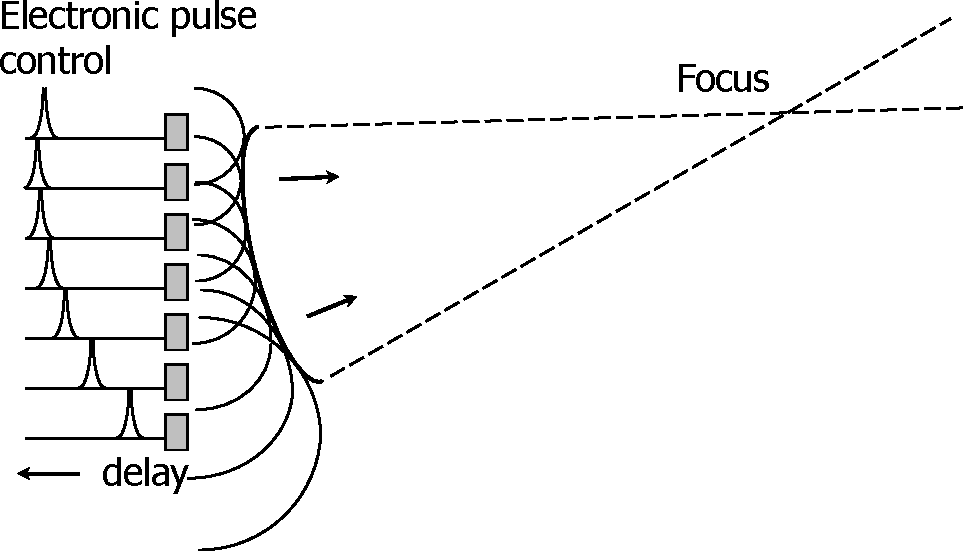
\includegraphics[width=.9\linewidth]{Figures/Ultrasound/ultrasound_focused_beam_v2.pdf}
  \captionof{figure}{Generating a focused wave front by adjusting the delays at which the individual piezoelectric elements in the transducer generate the ultrasound wave. The focus point can be directed at an arbitrary location.}
  \label{fig:us_focus_beam}
\end{minipage} $\quad$
\begin{minipage}[t]{.48\textwidth}
  \centering
    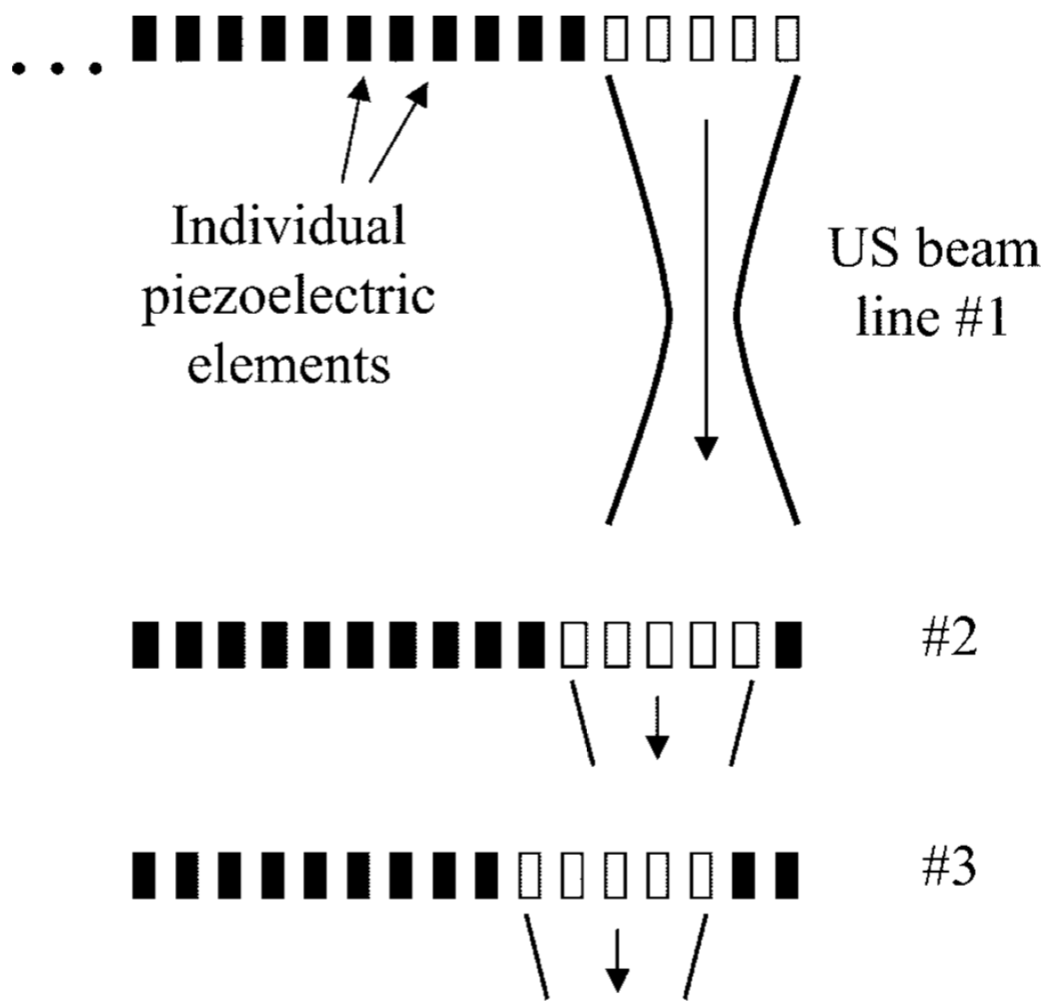
\includegraphics[width=.75\linewidth]{Figures/Ultrasound/conventional_line_scanning.png}
    \caption{The process of line-by-line scanning in conventional ultrasound. The imaging speed depends both on the depth of the object to image (acoustic travel time) and on the number of lines to scan (width of the resulting image). Figure adapted from \citet{hangiandreou_aapm/rsna_2003}.}
    \label{fig:us_line-by-line}
\end{minipage}
\end{figure}


% The process acquiring an image in the conventional method by generating a focused beam, measuring its reflection, and repeating this for the number of desired horizontal image lines, 
The described process of acquiring the ultrasound image, is also known as line-by-line scanning. The frame rate of this conventional method is limited by the number of desired scanning lines and the depth of the object to image. The time it takes to acquire one image is given by,
\begin{equation}
    T_\text{image} = \frac{2 \, z \, N_\text{lines}}{c},
\end{equation}
with $z$ the depth of the object to image, $N_\text{lines}$ the number of lines and $c$ the speed of sound through the medium, usually around \SI{1540}{\meter\per\second} in soft tissue. This already shows that the imaging frame rate for superficial tissue at e.g. \SI{5}{\centi\meter} with 256 lines is limited to \SI{60}{\hertz}. 

There have been several attempts to speed up the imaging speed in conventional ultrasound, for example a technique called ``explososcan''. With this technique, a slightly unfocused beam is emitted, and the recorded echo can be used to parallel process 4 lines from one transmit \cite{shattuck_explososcan_1984}. This increases the imaging speed by a factor four, at cost of image quality. However, for some applications, e.g. tracking and analysis of heart motion, this increase in frame rate is insufficient. 




% -----------------------------------------------------------------------
\subsection{Plane wave ultrafast ultrasound}
Ultrafast ultrasound (or plane wave ultrasound) uses plane waves (i.e. unfocused waves) to insonify the complete region of interest. Part of the plane wave will be reflected or scattered by the object, and the resulting backscattered echoes are recorded by the piezoelectric elements in the transducer. Each element records a different echo and converts the sound waves to Radio Frequency (RF) signals. These RF signals can then be used to reconstruct the image of the insonified object, due to the fact that acoustic waves can be time reversed. Although this may sound very similar to the conventional method, the underlying principle from physics is very different. Since there is no need for a focussed wave, the entire image can be acquired from a single insonification by parallel beamforming of the RF data. This speeds up the image acquisition time tremendously. 
%This appears similar to conventional ultrasound, however, since there is no need for a focused wave, all lines of the image can be acquired at the same time by parallel beamforming, speeding up the image acquisition time tremendously. 
% via a technique called time reversal. 

\subsubsection{Time reversal of acoustic waves}
The time reversal technique is based on the fact that the propagation of ultrasonic and sonic acoustic waves is a reversible process \cite{tanter_time_2009}. This phenomenon is utilised in the Time Reversal Mirror (TRM), which is made of an array of reversible transducers (e.g. a surface covered with piezoelectric elements in case of ultrasound). From any given emitting source, the TRM first records the emerging waves into memory, after which these recordings are time reversed, and the reversed recording is then transmitted by the TRM transducers (i.e. first in, last out). This will result in the exact reverse of the emitted wave field, as depicted in \autoref{fig:us_time_reversal_mirror}, with presence of an arbitrary obstacle. 

\begin{figure}[t]
    \centering
    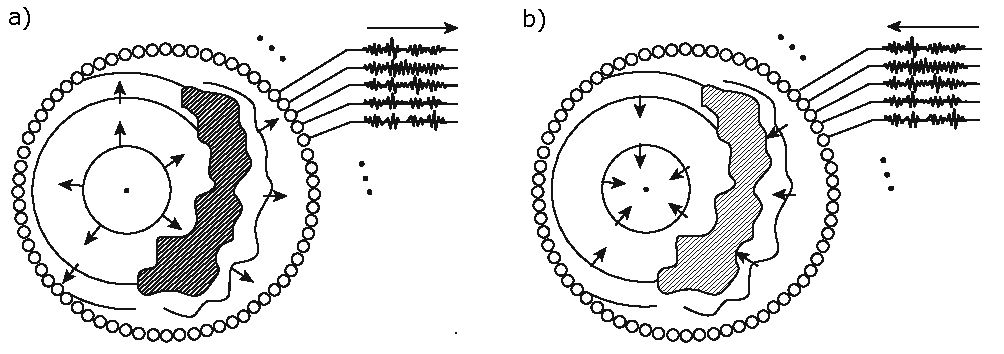
\includegraphics[width=\linewidth]{Figures/Ultrasound/time_reverval_mirror_2.pdf}
    \caption{\textbf{(a) Receiving:} The acoustic waves emitted by a point in the centre travel through the medium, resulting in a distorted wave front, which is then recorded by the Time Reversal Mirror (cylindrical array of piezoelectric transducers). \textbf{(b) Transmitting:} Next the recording is reversed (i.e. time reversal step), and is emitted by the transducers. The wave field will travel through the object, and will refocus exactly at the location of the initial source. Figure adapted from \citet{tanter_time_2009}.}
    \label{fig:us_time_reversal_mirror}
\end{figure}


In the discussed case, a propagating wave field is first recorded and then re-emitted to obtain the reverse field. Due to the reversibility of propagating acoustic waves, the inverse is also possible, i.e. first emitting a wave field and subsequently recording the echoes. Instead of physically generating the time reverse of the wave field, it is also possible to computationally reconstruct what caused the backscattered echo, based on one transmission of a known wave field, by performing digital parallel beamforming of the echoes \cite{tanter_ultrafast_2014}.




\subsubsection{Digital parallel beamforming}

\begin{figure}[!b]
    \centering
    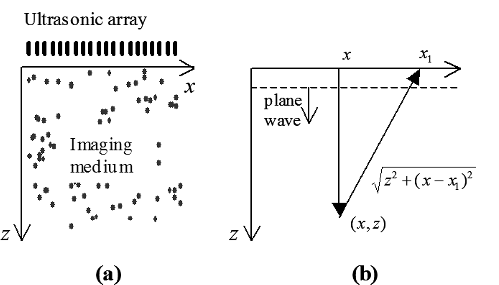
\includegraphics[width=.5\linewidth]{Figures/Ultrasound/beamforming_geo.pdf}
    \caption{Overview of the geometry for calculation of the time delays for a plane wave for an arbitrary point at $(x,y)$ and a transducer located at point $x_1$. Figure adapted from \citet{montaldo_coherent_2009}.}
    \label{fig:us_beamforming_geo}
\end{figure}

% In order to get from raw recorded RF signals to an image, the echoes are numerically backpropagated by a technique called (digital) parallel beamforming (PBF) \cite{tanter_ultrafast_2014}. 
% \textcolor{red}{This method is already fairly old, and newer and better have been developed (e.g. minimum variance beamforming \cite{holfort_plane_2008}). These will not be discussed, because of the complexity of these methods.}
In order to get from raw recorded RF signals to an image, the recorded echoes of the individual elements are beamformed using e.g. the \textit{delay-and-sum} method (DAS, also D\&S or DS). Since there is no focusing in plane wave ultrasound, the image has to be reconstructed by coherently summing the backscattered echoes. For a point $(x,y)$ the travelling time to this point and from this point back to element $i$ at $x_i$ is given by,
\begin{equation}
    \tau \left( x_i, x, z \right) = \frac{z + \sqrt{z^2 + {\left( x- x_i \right)}^2 }}{c},
\end{equation}
with $c$ the speed of sound, assumed constant in the medium \cite{montaldo_coherent_2009}. This situation is depicted in \autoref{fig:us_beamforming_geo}. Each pixel in the image will be reconstructed by first delaying the RF signals with a cylindrical time delay (based on the transducer location with respect to the pixel location), and then coherently summing the delayed signals of each transducer with an aperture weighting \cite{tanter_ultrafast_2002}. For a transducer with $N$ elements, with each element $i$ receiving RF signal $r_i(t)$, the beamformed RF signal from line $x$ becomes, 
\begin{equation}
    r_{BF} \left( x, z\right) = \sum_{i=0}^{N-1} \alpha\left(i,x,z \right) r_i \left(  t \left( x_i, x, z \right) \right),
\end{equation}
with $\alpha(i,x,z)$ the apodization factor, depending on the location of the pixel to beamform and the element number \cite{holfort_broadband_2009}. The apodization factor weights for each pixel to reconstruct how much the raw RF signal from the individual elements has to contribute. In DAS beamforming, the apodization factor is usually based on element directivity. Incident waves with a large angle (large deviation from the perpendicular) are penalised due to their low signal-to-noise ratio (SNR) \cite{chen_improved_2018}. % In general, probe elements are more sensitive to waves with small angular deviation from the perpendicular (,  \cite{chen_improved_2018}.
% which means that elements are more sensitive to waves received at small angles \cite{chen_improved_2018}.

More recently developed beamformers, such as the \textit{minimum variance} (MV) beamformer \cite{holfort_plane_2008}, the \textit{delay multiply and sum} (DMAS) beamformer \cite{matrone_delay_2015} and \textit{Stolt's f-k migration} \cite{garcia_stolts_2013} have proven to be able to reconstruct images with better resolution and contrast than the conventional DAS beamformer. The differences are mostly caused by using data dependent apodization weights, instead of fixed apodization weights based on merely the pixel location and transducer element as used in DAS. The adaptive MV beamformer, uses apodization weights based on the frequency content of the recorded RF signals, and continuously updates these weights \cite{holfort_plane_2008}. The DMAS is a nonlinear beamformer, taking the spatial cross-correlation among all the recorded RF signals of all the transducers at each time instant \cite{matrone_delay_2015}. This again results in a data dependent beamforming by using a measure for the backscattered signal coherence. %\textcolor{red}{\textit{Stolt's f-k migration} \cite{garcia_stolts_2013}}

% \typeout{msg}
% XXX note: use image Montaldo (\cite{montaldo_coherent_2009})?
\bigskip




% -----------------------------------------------------------------------
\subsection{Enhancing image quality}
A disadvantage of plane wave imaging is the loss in contrast and resolution, which is caused by the lack of focus in the transmitted wave \cite{montaldo_coherent_2009}. In order to improve the image quality, various compound imaging methods can be used. 


\subsubsection{Incoherent wave compounding}
By incoherently combining several consecutive frames the effect of noise can be reduced, similar to time domain averaging resulting in increased signal-to-noise ratio. This method is also referred to as real-time spatial compound imaging. Each individual frame is formed of a plane wave under an angle, by means of electronic beam steering. The waves are emitted in a predetermined sequence of angles, usually between 3 an 9 different angles. Next, the frames are combined into an image as depicted in \autoref{fig:us_spatial_compounding}. By having multiple viewing angles, artefacts resulting from one specific view angle are suppressed by the averaging step \cite{entrekin_real-time_2001}. This results in images with less speckle, clutter and other acoustic artefacts. The frame rate is not reduced, since previous recorded frames will be used to enhance the new frame. This can however lead to blurry images, when the tissue or transducer is moving too fast. Since the waves are emitted under an angle, not the entire image can be compounded, meaning that the edges of the image might still contain artefacts \cite{entrekin_real-time_2001}. 

\begin{figure}
    \centering
    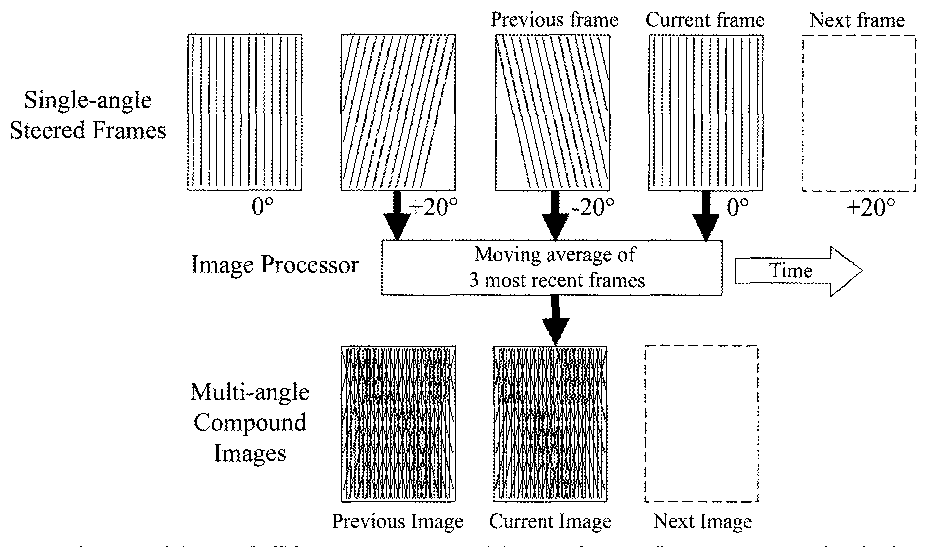
\includegraphics[width=.8\linewidth]{Figures/Ultrasound/spatial_compounding.pdf}
    \caption{Incoherent compound imaging, or real-time spatial compound imaging. Individual frames are made from a single plane wave under an angle. The new image will be composed of the newest acquired frame and the previous $n-1$ frames, with $n$ representing the number of different angles, typically between 3 and 9. Figure adapted from \citet{entrekin_real-time_2001}.}
    \label{fig:us_spatial_compounding}
\end{figure}



\subsubsection{Coherent wave compounding}
In coherent wave compounding, not a combination of beamformed frames is used to create an enhanced image, but the raw received backscattered echoes (RF signals) of multiple plane wave transmits under an angle are combined. The transmit and receive process is similar to incoherent plane wave compounding, but the processing of the received echoes is different. By emitting plane waves under a sequence of angles, the lack of focus can artificially be compensated. By changing the delays of the individual received echoes and summing them coherently, focusing can be performed synthetically at any arbitrary location as depicted in \autoref{fig:us_coherent_compounding}. 

When coherent compounding, the image cannot be formed in real-time, since first all the backscattered echoes need to be recorded, after which the synthetic focusing has to take place. This is a computationally very demanding process and therefore hard to implement in real-time imaging \cite{yiu_gpu-based_2011}. It also reduces the frame rate by the number of angles used. Therefore, for each specific application there is a trade-off in image contrast and resolution versus frame rate. The influence of the number of angles on the image quality is illustrated in \autoref{fig:us_compound_num_angles}. Like in incoherent wave compounding, imaging of fast moving objects can result result in blurry images, though there are methods proposed to compensate for motion using tissue Doppler imaging to estimate the motion of the tissue between successive transmits \cite{poree_high-frame-rate_2016}. 

\begin{figure}
	\centering
	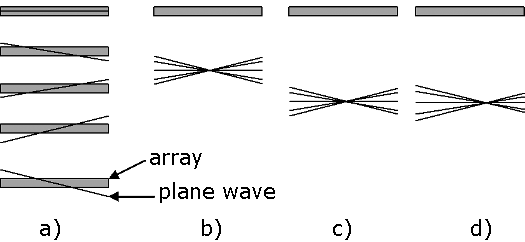
\includegraphics[width=.6\linewidth]{Figures/Ultrasound/coherent_compounding.pdf}
	\caption{In coherent compound imaging focusing can be performed synthetically, by adding the echoes of plane waves with adequate delays. \textbf{(a)} plane waves are emitted under different angles, \textbf{(b)}, \textbf{(c)}, \textbf{(d)} by tweaking the delays the focus point can be changed in both lateral and axial direction. Figure adapted from \citet{montaldo_coherent_2009}.}
	\label{fig:us_coherent_compounding}
\end{figure}


\begin{figure}
    \centering
    \includegraphics[width=\linewidth]{Figures/Ultrasound/compound_num_angles.pdf}
    \caption{Comparison of the effect of coherent plane wave compounding with multiple angles on image quality. The numbers below the number of planes represent the frame rate. Figure adapted from \citet{montaldo_coherent_2009}.}
    \label{fig:us_compound_num_angles}
\end{figure}





% =======================================================================
\subsection{Ultrafast ultrasound compared to conventional ultrasound}
As shown before, ultrafast ultrasound can be a lot faster than conventional ultrasound, due to the fact that the image is acquired by one single plane wave insonification, instead of multiple focused beams. This reduces the acquisition time of the image by the number of scanning lines used in the conventional method. Therefore, the (theoretical) minimum acquisition time per frame in the ultrafast case becomes, 
\begin{equation}
	T_\text{image} = \frac{2 \, z}{c},
\end{equation}
thus only dependent on the imaging depth. In \autoref{tab:us_conv_plane_wave_theoretical_comp}, the theoretical frame rate of conventional and ultrafast ultrasound is stated for a number of clinical applications. Imaging with unfocused waves has a disadvantage. If a plane wave image is compared to a line-by-line scanned image, the plane wave image is of lower quality. To improve the image quality, compound imaging can be used, at cost of frame rate. 


% Table generated by Excel2LaTeX from sheet 'Sheet1'
\begin{table}[t]
  \centering
  \caption{Comparison of theoretical imaging rate for different clinical applications. Conventional ultrasound frame rates are based on 128 scanning lines. Table adapted from \citet{minin_ultrafast_2011}.}
    \begin{tabular}{lccc}
    \toprule
    \multicolumn{1}{p{8.18em}}{Application} & \multicolumn{1}{p{7.5em}}{Typical imaging depth [cm]} & \multicolumn{1}{p{7.5em}}{Conventional frame rate [Hz]} & \multicolumn{1}{p{8.5em}}{Ultrafast imaging rate [Hz]} \\
    \midrule
    Abdominal imaging & 20    & 20    & 3800 \\
    Cardiac imaging & 15    & 150   & 5000 \\
    Breast imaging & 5     & 60    & 15000 \\
    \bottomrule
    \end{tabular}%
  \label{tab:us_conv_plane_wave_theoretical_comp}%
\end{table}%



% Table generated by Excel2LaTeX from sheet 'Sheet1'
\begin{table}[t]
  \centering
  \caption{Comparison of different imaging techniques. Table adapted from \citet{montaldo_coherent_2009}.}
    \begin{tabular}{lcccc}
    \toprule
          & \multicolumn{1}{l}{Resolution [mm]} & \multicolumn{1}{l}{Frame rate [Hz]} & \multicolumn{1}{l}{Contrast [dB]} & \multicolumn{1}{l}{SNR [dB]} \\
    \midrule
    Line scanning (128 lines) & 1.1   & 100   & 32    & 18 \\
    Plane wave & 1.8   & 12500 & 12    & 0 \\
    Compound 12 & 1.1   & 1000  & 20    & 11 \\
    Compound 45 & 1.1   & 270   & 30    & 16 \\
    Compound 71 & 1.1   & 176   & 33    & 18 \\
    \bottomrule
    \end{tabular}%
  \label{tab:us_conv_plane_wave_comparison}%
\end{table}%

In \autoref{tab:us_conv_plane_wave_comparison} plane wave imaging is compared with coherent compound imaging and conventional line-by-line scanning. The methods are compared in resolution and contrast (i.e. image quality), frame rate and SNR (relative to single plane wave imaging). The comparison is based on a superficial tissue mimicking phantom (focus depth approx. \SI{30}{\milli\meter}). From the table it becomes clear that coherent compound imaging using 45 angles gives similar image quality as conventional ultrasound, but with improved frame rate. It should be noted that \citeauthor{montaldo_coherent_2009} used a conventional DAS beamformer \cite{montaldo_coherent_2009}. More recently developed beamformers further improve the image quality, meaning that less angles have to be used to reach similar contrast and resolution \cite{chen_improved_2018}.




% =======================================================================
\section{Applications}
The ultrafast imaging rate of plane wave ultrasound has opened up possibilities in multiple clinical applications; elastography, blood flow analysis and functional brain imaging. In this section, these new possibilities will be introduced. Since it is expected that elastography can be useful in system identification experiments, this application is discussed more in depth. The other applications, blood flow analysis and measuring brain activity, are only discussed briefly. 



% -----------------------------------------------------------------------
\subsection{Ultrafast Doppler Blood Flow Analysis}
In conventional ultrasound, two Doppler modes for blood flow analysis are available. The first mode, spectral analysis Doppler, is based on the spectral analysis of the received Doppler signal with respect to some excitation signal, a pulsed wave (PW) or continuous wave (CW). In this mode, measures such as peak flow velocity as function of time, mean flow velocity as function of time and resistance of the artery can be obtained. These measures require high frequent imaging, and thus a high temporal resolution is required which in conventional ultrasound results in a low spatial resolution. As a consequence of the limited frame rate in conventional ultrasound, in spectral analysis Doppler only one location is scanned (or multiple locations along the same line, i.e. multigating). The second mode is colour-coded flow velocity imaging, in which mean flow velocities over a larger region of interest (ROI) can be measured. Due to the higher required spatial resolution, the temporal resolution is lower. Hence, colour flow imaging results in a more qualitative measurement, mostly used to detect abnormalities in the blood flow pattern \cite{tanter_ultrafast_2014}. % In the second mode, colour flow imaging (CFI), the spatial resolution is higher at cost of temporal resolution. By scanning multiple lines a region of interest (ROI) can be analysed, but only mean flow velocities can be measured. Hence it is more a qualitative measurement, 

Physicians ideally use both these Doppler modes and normal imaging (B-mode) simultaneous in real-time, which is impossible with conventional ultrasound. Fortunately, the high frame rates of plane wave ultrasound open up new possibilities, allowing imaging and quantitative blood flow measurements simultaneously \cite{minin_ultrafast_2011}. By performing the Doppler analysis after the image acquisition, the physician is able to adjust the position of the PW Doppler ROI digitally after the exam, instead of manually moving the transducer or selecting another ROI during the examination. Consequently, multiple ROIs can be selected in the recorded image, without the need for successive exams, resulting in shorter examinations for the patient \cite{tanter_ultrafast_2014}. Furthermore, ultrafast ultrasound improves the sensitivity of the blood flow measurement significantly \cite{minin_ultrafast_2011}. 
% It is also possible to create a complete mapping of the vascular system in e.g. the brain. 



% -----------------------------------------------------------------------
\subsection{Ultrafast Doppler Imaging of Brain Activity}
% Standard imaging techniques today allow deep brain imaging (e.g. EEG, PET and fMRI). For example, fMRI can be used to perform functional imaging deep in the brain, even able to measure increases in blood-oxygen levels ...
Another field in which ultrafast ultrasound shows new possibilities is in neuroscience. Standard imaging techniques today allow deep brain imaging (e.g. EEG, PET and fMRI), but their use is limited. These techniques have limitations in temporal resolution and signal-to-noise ratio at high spatial resolutions. Furthermore, the size of the imaging equipment limits its use in the operating room for monitoring brain activity \cite{tanter_ultrafast_2014}. 

Conventional ultrasound (PW Doppler) is not sensitive enough to measure blood flow in small vessels in the brain, but with the introduction of ultrafast ultrasound the sensitivity is significantly increased. By using ultrafast Doppler, plane wave ultrasound can be used to measure subtle changes in blood flow in the brain, which could provide new information regarding stroke \cite{tanter_ultrafast_2014}. The use of ultrafast ultrasound in brain functional imaging is also referred to as fUltrasound, in analogy with fMRI. The disadvantage of fUltrasound is that its use is limited due to the skull distorting or even blocking the propagation of the ultrasound waves. Therefore, the application is currently limited, but shows great potential for monitoring brain activity in newborns through the fontanel window, and in adults duing neurosurgery \cite{tanter_ultrafast_2014}. 




% -----------------------------------------------------------------------
\subsection{Elastography -- Supersonic shear wave imaging}
\label{sec:us_ssi}
Elastography is the first clinical application of ultrafast ultrasound. Elastography is an imaging method used to map tissue stiffness, and has been under development since the 1990's \cite{gennisson_ultrasound_2013}. It was developed to replace manual palpation by clinicians, and shift from qualitative estimation of the elastic tissue properties to a more quantitative estimation. Elastography can be divided in quasi-static and dynamic methods. 

In the quasi-static method, only a qualitative map can be made of tissue strain. Some constant force is externally applied to compress the tissue, resulting in constant stress in the tissue. Ultrasound images (usually conventional line-by-line scanning) are acquired without force present and next with the compressing force. By tracking the displacement of the tissue, a strain map can be generated. Following Hooke's law, $\sigma = E \epsilon$, it is known that the strain is proportional to the stress (assuming that the tissue behaves linear-elastic). Using this method, the Young's modulus $E$ cannot be found, and only a qualitative strain mapping can be made \cite{gennisson_ultrasound_2013}. 

The dynamic methods can be used in a more quantitative way to determine the elastic properties. There are several dynamic elastography methods, vibro-acoustography, acoustic radiation force imaging (ARFI), 1D transient elastography, 2D transient elastography and supersonic shear wave imaging (SSI). Only the latter uses ultrafast ultrasound imaging, the others rely on conventional ultrasound. All methods based on conventional ultrasound face the same limitations as the other discussed applications, i.e. a strict trade-off in temporal resolution versus spatial resolution. %limited temporal resolution at high spatial resolution and vice versa. 
In dynamic elastography a time varying force perturbation (transient or oscillatory) is induced by the ultrasound transducer, or some other (mechanical) transducer. This perturbation will result in a shear wave in the tissue, typically with a frequency between 10 and 2000 \si{\hertz} \cite{gennisson_ultrasound_2013}. By following this shear wave in the acquired ultrasound images, the propagation velocity of the wave can be found. From this, the elastic properties of the tissue can be determined.

In all dynamic elastography methods, the tissue is assumed to behave as a linear elastic material. In purely elastic media, the phase velocity is independent of shear wave frequency. Consequently, when performing dynamic elastography, only the elastic properties of the medium can be estimated. If the material behaves viscoelastic, shear wave spectroscopy (SWS) can be performed, which will be discussed in \autoref{sec:us_sws}.




\begin{figure}[t]
    \centering
    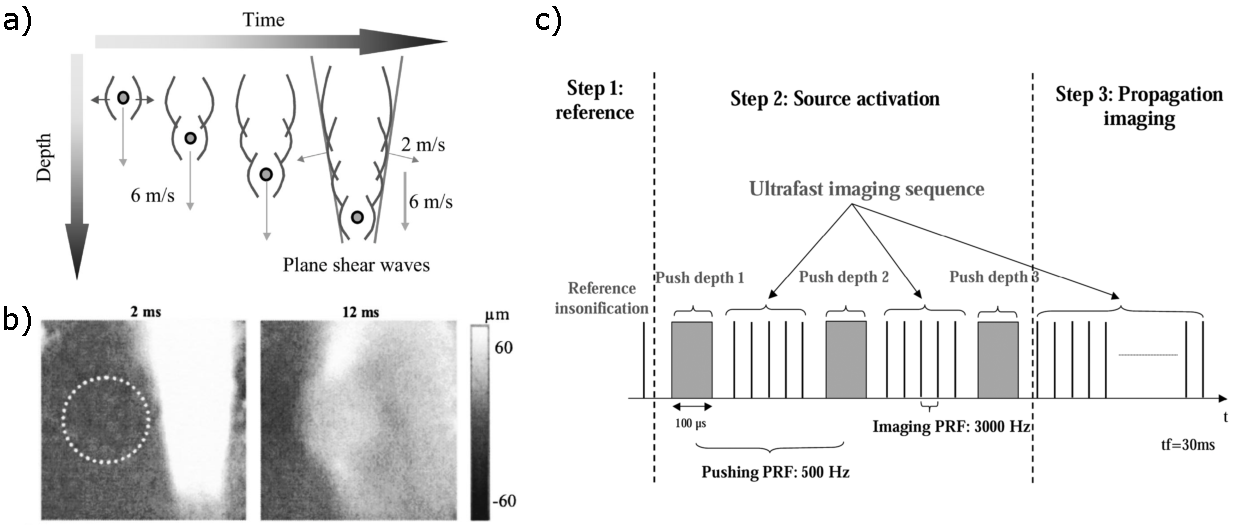
\includegraphics[width=\linewidth]{Figures/Ultrasound/us_shear_wave_imaging.pdf}
    \caption{\textbf{(a)} Generation of the Mach cone by `pushing' multiple focused beams at different depths, constructive interference results in the plane shear wave front. \textbf{(b)} Propagation of the shear wave through a tissue-mimicking phantom (agar-gelatin), with a \SI{20}{\milli\meter} diameter hard inclusion. \textbf{(c)} emission sequence in supersonic shear wave imaging. Figures \textbf{(a,b)} adapted from \citet{bercoff_sonic_2004} and \textbf{(c)} from \citet{bercoff_supersonic_2004}.}
    \label{fig:us_mach_cone}
\end{figure}

% \tred[XXX]
\subsubsection{Supersonic shear wave imaging}
In supersonic shear wave imaging (SSI) the mechanical perturbation that results in the shear wave is induced by the ultrasound transducer using acoustic radiation pressure. The shear wave is created by successively focusing the ultrasonic probe at different depths. Consequently, the resulting shear waves will interfere constructively, and form a Mach cone. In the imaging plane, this can be seen as two shear waves propagating in opposite direction (depicted in \autoref{fig:us_mach_cone}a and b) \cite{bercoff_sonic_2004}. The use of this constructive interference increases the amplitude of the shear wave (compared to single focusing), hence resulting in a higher SNR of the displacement field \cite{gennisson_ultrasound_2013}. The order of displacement is about \SI{40}{\micro\meter} \cite{bercoff_sonic_2004}. Since the induced shear wave travels within the range of 1--10 \si{\meter\per\second}, an imaging rate of minimal \SI{1000}{\hertz} is required to follow this wave \cite{minin_ultrafast_2011}. These frame rates are only possible at high spatial resolution by using ultrafast ultrasound. 
% frequency not too high, otherwise attenuation... ?

The sequence in which SSI is performed is depicted in \autoref{fig:us_mach_cone}c. In the first step, a reference image is formed, used to determine the displacements induced by the shear wave. In the second step, the supersonic source is activated by successive focusing a beam at multiple depths (4 depicted in \autoref{fig:us_mach_cone}a and 3 in \autoref{fig:us_mach_cone}c). After each push at the designated depth, ultrafast imaging can be performed to follow the formation of the Mach cone and propagation of the shear wave. After shear wave pushing is completed, ultrafast imaging can be performed to follow the shear wave. The total sequence for a single SSI measurement takes less than \SI{30}{\milli\second} \cite{bercoff_supersonic_2004}. It should be noted that the first images after generation of the shear wave cannot be used, since the pushing beam itself is backscattered. This blinds the probe momentarily, resulting in approximately   \SI{0.5}{\milli\second} of dead time after shear wave pushing during which no usable images can be reconstructed \cite{deffieux_shear_2009}.
% The difference in propagation speed between compressional waves and shear waves is sufficiently large, that imaging using ultrafast ultrasound does not interfere with the 


\subsubsection{Assumptions from material science}
There are two types of mechanical waves that can propagate through soft tissue: compressional waves (also called longitudinal waves, used for ultrasound imaging) and shear waves. These two types of waves have very different propagation speeds through soft tissue, for compressional waves about \SI{1500}{\meter\per\second} versus about \SI{10}{\meter\per\second} for shear waves. This is caused by the fact that the bulk modulus $\lambda$ of soft tissue is much higher (factor $10^6$) than the shear modulus $\mu$ \cite{minin_ultrafast_2011}. 

Soft tissues are often characterised as fluid-like solids. If it is assumed that soft tissue behaves like an isotropic linear elastic material, its properties can be expressed in terms of two parameters, bulk (compressional) modulus and shear modulus \cite{sarvazyan_biophysical_1995}. Two other mechanical parameters, Young's modulus $E$ and Poisson's ratio $\nu$, are related to $\lambda$ and $\mu$,
\begin{equation}
    \label{eq:K}
    \lambda = \frac{E}{3(1-2\nu)},
\end{equation}
\begin{equation}
    \label{eq:G}
    \mu = \frac{E}{2(1+\nu)}.
\end{equation}
By combining these equations, an expression for the Young's modulus can be found in terms of $\lambda$ and $\mu$, 
\begin{equation}
    E = \frac{9 \mu \lambda}{(\mu + 3 \lambda)}.
\end{equation}
Then using the assumption that the bulk modulus is a factor $10^6$ larger than the shear modulus ($\lambda \gg \mu$), the Young's modulus $E$ (measure for tissue elasticity) can be expressed as,
\begin{equation}
    E = \frac{9 \lambda \mu}{3\lambda + \mu} \approx 3 \mu.
\end{equation}
By using the relation between shear wave propagation speed $c_g$ (group velocity), shear modulus and density of the tissue $\rho$, $\mu = \rho {c_g}^2$, the relation between the Young's modulus and shear wave propagation speed is found,
\begin{equation}
    E = 3 \mu = 3 \rho \, {c_g}^2.
\end{equation}
Concluding, by assuming that soft tissue behaves like an isotropic linear elastic material, the tissues Young's modulus $E$ can be estimated by the propagation speed of a shear wave in tissue. 

In reality, soft tissue is not behaving linear and isotropic, and the elastic moduli are not time invariant. However, according to \citeauthor{sarvazyan_biophysical_1995} this very simplistic model is quite adequate, and depending on the problem can be advantageous over more complex models that require many material parameters \cite{sarvazyan_biophysical_1995}.

% Elastograpgy gaat ervanuit dat alle materialen homogeen / isentroop zijn. tendon (connective tissue) is anisotropic, and anisotropy can cause a different amount of ultrasound reflection, depending on the angle of the incident ultrasound wave. 
% Tegenstrijdig hoe Elastography werkt en imaging van tissue.



\subsection{Elastography -- Shear wave spectroscopy}
\label{sec:us_sws} %\tred 
% \subsubsection{Shear wave spectroscopy}
In linear elastic media, the phase velocity of a shear wave is equal to its group velocity. For viscoelastic media such as breast and liver tissue, the phase velocity increases as a function of frequency (i.e. dispersion), which means that a different rheological model and measurement method has to be used to determine its material properties \cite{minin_ultrafast_2011}. In SSI, the shear modulus $\mu$ can be estimated by merely looking at the wave's group velocity, hence millimeter resolution suffices. SWS on the other hand, relies on estimation of the phase velocity which requires a higher resolution and SNR, since the amount of energy for the individual frequency components is lower than the total energy of the signal \cite{deffieux_shear_2009}. For a high SNR and resolution, it is beneficial to take a relatively large ROI of \SI{1}{\centi\meter\squared}, since smaller ROIs result in a larger variance on the estimation of the shear wave velocity. Within this ROI, the tissue is assumed to be homogeneous for the SWS analysis. Since there is about \SI{0.5}{\milli\second} of dead time after shear wave pushing, it is important to locate the ROI at a lateral distance of approximately \SI{4}{\milli\meter} from the pushing line, allowing imaging of the shear wave propagation in the complete ROI. 

\citeauthor{deffieux_shear_2009} first introduced SWS, by using an experimental setup able to perform one complete SSI experiment within \SI{200}{\milli\second} (\SI{25}{\milli\second} of shear wave pushing and imaging, additional time is required for transferring data, beamforming, speckle tracking and velocity map building) \cite{deffieux_shear_2009}. This setup allowed performing 10 successive SSI experiments in 2 seconds. The 10 acquired velocity fields $u(x,z,t)$ were averaged to increase the SNR. The resulting velocity field was further averaged along the $z$ direction (depth, see \autoref{fig:us_sws_wave_propagation}), to obtain the velocity field $u(x,t)$. Taking the Fourier transform of the velocity field $u(x,t)$ results in $U(x,\omega)$, which can be divided in phase $\varphi(x,\omega)$ and amplitude $A(x,\omega)$ of the wave for each frequency $\omega$ at location $x$. 


% Figures SWS
\begin{figure}[t]
% \centering
\begin{minipage}[t]{.48\textwidth}
  \centering
  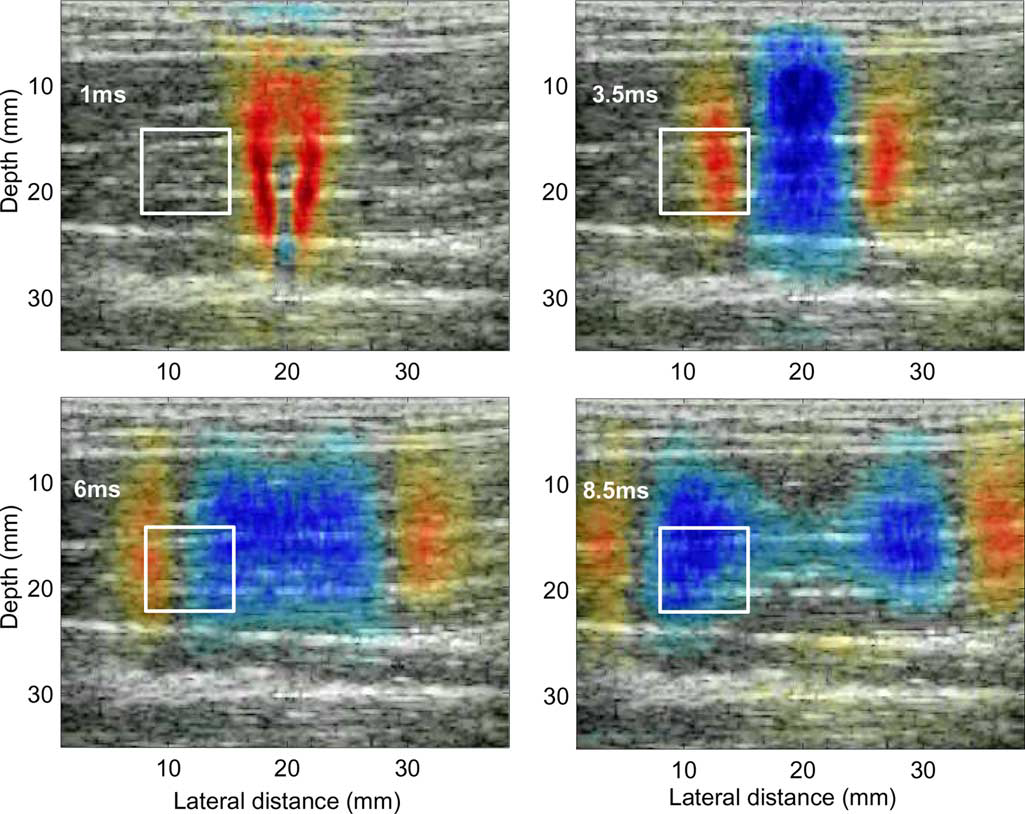
\includegraphics[width=\linewidth]{Figures/Ultrasound/us_sws_wave_propagation_muscle.png}
  \captionof{figure}{Propagation of a shear wave along muscle fibres of the \textit{biceps brachii}. Two quasi-plane waves propagate in opposite direction, causing maximum relative tissue displacement of around \SI{10}{\micro\meter} between successive images at a frame rate of \SI{4000}{\hertz}. The colour scale represents the tissue velocity in the $z$ (depth) direction. The colour scale has been re-normalised for each individual image for clear visualisation of the shear wave, since the amplitude slowly decreases over time. Figure adapted from \citet{deffieux_shear_2009}.}
  \label{fig:us_sws_wave_propagation}
\end{minipage} $\quad$
\begin{minipage}[t]{.48\textwidth}
  \centering
    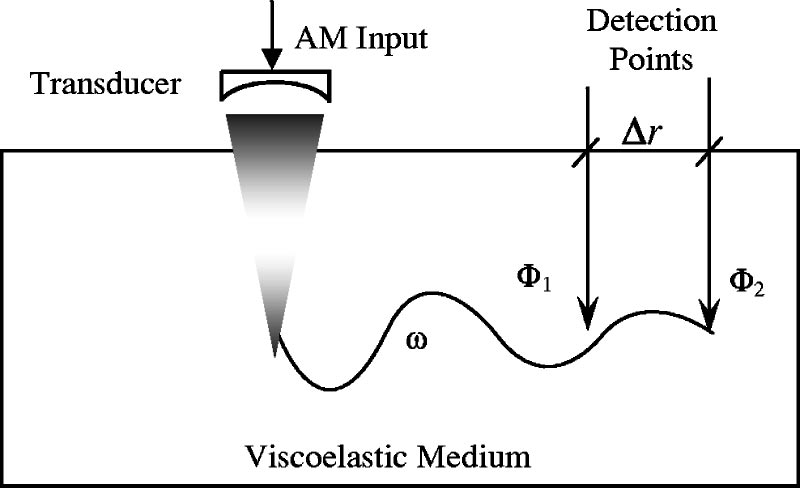
\includegraphics[width=\linewidth]{Figures/Ultrasound/us_sws_phase_diff.png}
    \caption{Concept of shear wave phase velocity estimation. The phase of the wave is measured at two locations at distance $\Delta r$. The shear wave's phase velocity $c_{\varphi}$ can be  determined by the phase shift ($\Delta \varphi = \varphi_1 - \varphi_2$), the frequency of the shear wave $\omega$ and the distance $\Delta r$. Figure adapted from \citet{chen_quantifying_2004}.}
    \label{fig:us_sws_phase_diff}
\end{minipage}
\end{figure}


To determine the phase velocity of the shear wave per frequency, the phase difference of the individual frequency components is determined over a certain distance $\Delta x$ (the width of the ROI). This way the phase velocity for frequency $\omega$ can be approximated by \cite{chen_quantifying_2004},
\begin{equation}
    c_{\varphi}(\omega) = \frac{\omega \, \Delta x}{\Delta \varphi}.
\end{equation}
Using this equation and the obtained phases $\varphi(x,\omega)$, the phase velocity $c_{\varphi}$ can be estimated for all frequency components. From this, the dispersion curves can be formed, and a rheological model can be fitted. The Voigt and Maxwell models are linear descriptions of a viscoelastic medium, comprising of a spring and damper in series (Maxwell) or parallel (Voigt) \cite{chen_quantifying_2004}. The Voigt model is often used to relate the phase velocity and frequency using the density $\rho$, shear elasticity $\mu_1$ and shear viscosity $\mu_2$,
\begin{equation}
    c_{\varphi}(\omega) = \sqrt{\frac{2\left( \mu_1^2+\omega^2 \mu_2^2\right)}{\rho \left( \mu_1 + \sqrt{\mu_1^2 + \omega^2 \mu_2^2} \right)}}.
\end{equation}
Assuming $\rho$ is known (and constant), the mechanical properties of the medium can be estimated by fitting this rheological model to the experimentally obtained dispersion curve \cite{deffieux_shear_2009}. With the estimated viscoelastic parameters, the stress $\sigma$ in the material can then be derived from,
\begin{equation}
	\sigma = \mu_1 \, \epsilon + \mu_2 \, \dot\epsilon,
\end{equation}
with $\epsilon$ the strain in the material. 

To obtain a usable dispersion curve, the generated shear wave should have sufficient bandwidth. The bandwidth of the shear wave is dependent on the properties of the medium, the ultrasound probe design and the insonification parameters (e.g. the angle of the shear wave) \cite{nguyen_assessment_2011}. As a consequence, the bandwidth varies depending on the application, and is reported to be $50-400$~\si{\hertz} in breast applications  \cite{nguyen_assessment_2011} and $100-800$~\si{\hertz} in muscle application (\textit{in vivo biceps brachii}) \cite{gennisson_viscoelastic_2010}.





% Shear wave spectroscopy (SWS) can be seen as an extension of SSI, and can be used to quantify both local shear elasticity and dispersion in real time \cite{deffieux_shear_2009}. 





% , hence a different method has be used to determine the viscoelastic properties. Shear wave spectroscopy
% When the shear wave is properly generated and imaged, the waves phase velocity and group velocity as function of frequency can be determined locally \cite{minin_ultrafast_2011}. For different tissue types, different rheological models can be used. The phase velocity is independent of frequency for purely elastic media, and is equal to the group velocity. On the other hand, and other rheological models can be used, depending on the frequency of the shear wave \cite{minin_ultrafast_2011}.

















% FIGURE TIMING DELAYS PLANE WAVE
% \begin{minipage}[t]{.48\textwidth}
%   \centering
%   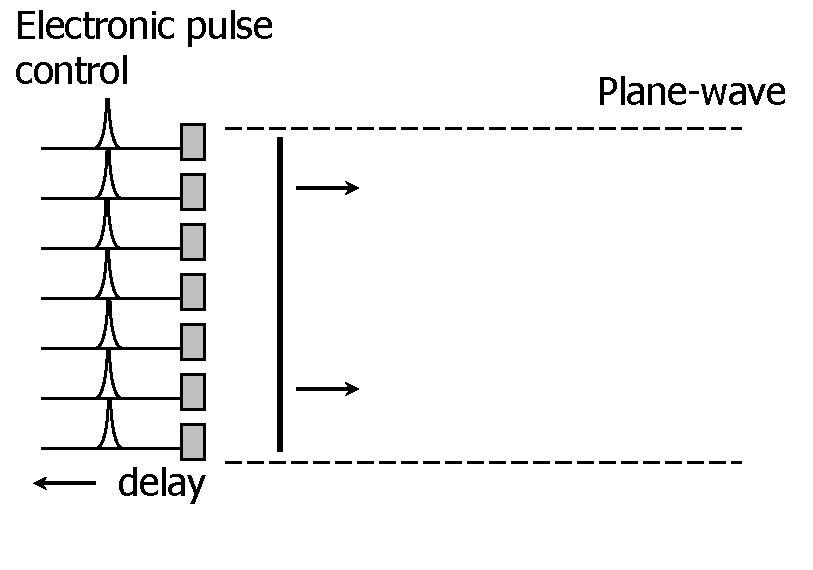
\includegraphics[width=.9\linewidth]{Figures/Ultrasound/ultrasound_plane_wave.pdf}
%   \captionof{figure}{In ultrafast ultrasound imaging a plane-wave front is generated by equal delays on all the piezoelectric elements in the transducer. }
%   \label{fig:us_plane_wave}
% \end{minipage}






% \begin{figure}[H]
%     \centering
%     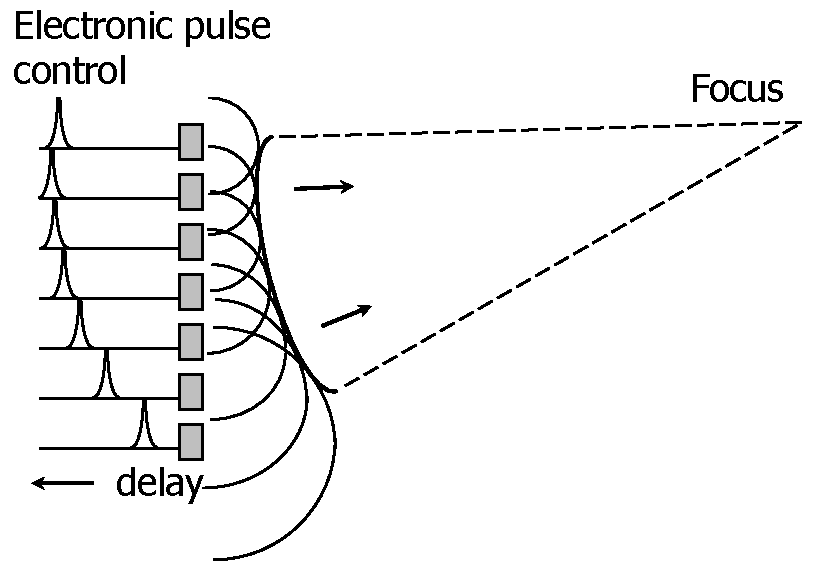
\includegraphics[width=.5\textwidth]{Figures/Ultrasound/ultrasound_focused_beam.pdf}
%     \caption{Generating a focused wave front by adjusting the delays at which the individual piezoelectric elements in the transducer generate the ultrasound wave. The focus point can be directed at any arbitrary location. }
%     \label{fig:us_focus_beam}
% \end{figure}


% \begin{figure}
% \centering
% \begin{subfigure}[t]{.5\textwidth}
%   \centering
%   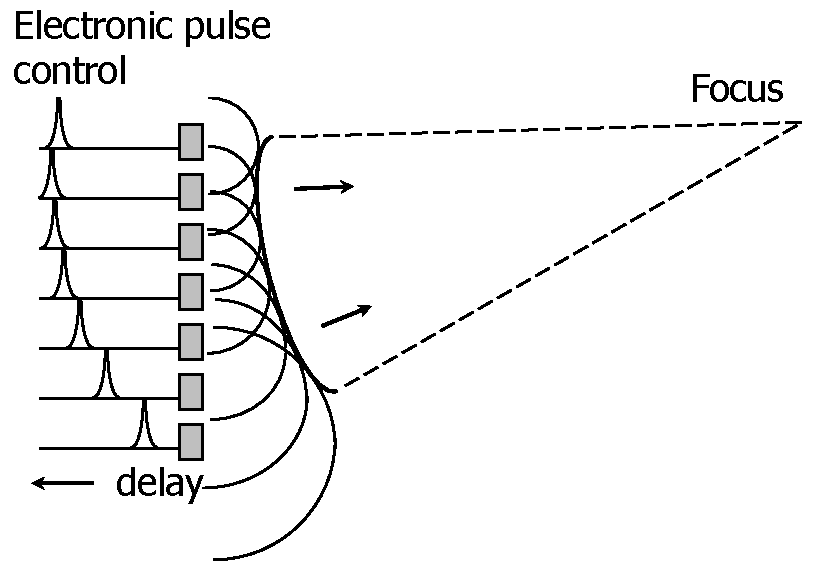
\includegraphics[width=.9\linewidth]{Figures/Ultrasound/ultrasound_focused_beam.pdf}
%   \caption{Generating a focused wave front by adjusting the delays at which the individual piezoelectric elements in the transducer generate the ultrasound wave. The focus point can be directed at any arbitrary location.}
%   \label{fig:us_focus_beam}
% \end{subfigure}
% \begin{subfigure}[t]{.5\textwidth}
%   \centering
%   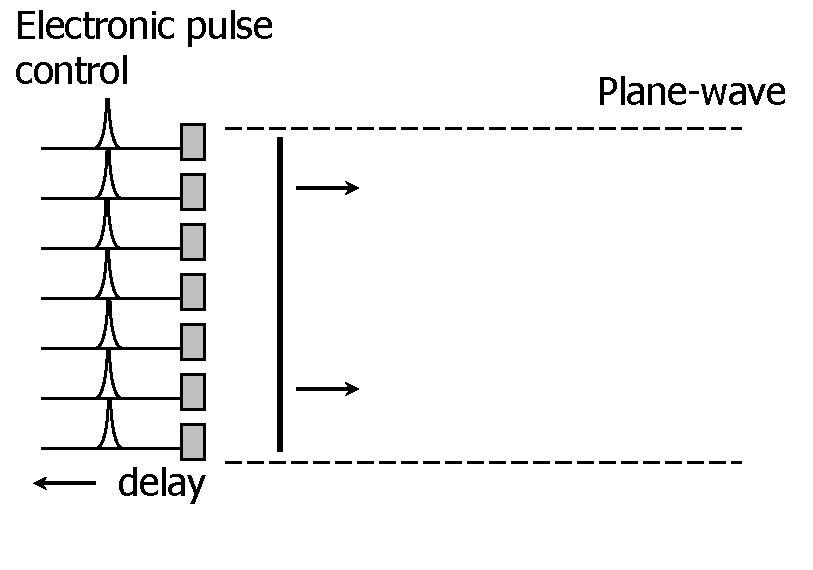
\includegraphics[width=.9\linewidth]{Figures/Ultrasound/ultrasound_plane_wave.pdf}
%   \caption{A subfigure}
%   \label{fig:sub2}
% \end{subfigure}
% \caption{Focused wave-front versus a plane-wave. }
% \label{fig:test}
% \end{figure}
% - passive and active intrinsic lumped, not individually estimated. (schouten had parameters, mugge threw them away)
% - others do same, specify stiffness and damping on joint level, not really considering stiffness / viscosity muscle. lumped larger system
% - intrinsic, no clear separation joint stiffness and damping (due to friction during movement) and muscle intrinsic properties. 
% - intrinsic short range stiffness (time variant or invariant discussion)


% time variant properties: 
% - thixotropy 
% - muscle fatigue (MVC for checking if fatigue happened) (duration of experiments arbitrary, no real check. MVC after e.g. relaxing tasks could be as high as beginning of experiment because of resting, but fatigue during trials can still be present.

\chapter{Assumptions in joint dynamics system identification}
\label{chap:assumptions}
A lot of different studies have been conducted to identify joint dynamics in the human body. The human neuromuscular system is complex, and the joint dynamics can be modulated by different mechanisms, in literature mainly separated into two components, intrinsic and reflexive feedback. To gain a better understanding in the contribution of these components and to determine the underlying physiology, many different models have been proposed. These models vary in complexity and resemblance to the presumed physiology of the human. A wide variety of assumptions have been introduced in studies to simplify the models, enabling identification of the introduced parameters. In this chapter the most important assumptions made in various studies are listed and compared to each other.

\tred[The considered studies all model the neuromuscular system as time invariant, though the effects of e.g. muscle thixotropy and short range stiffness have been described extensively in literature. These effects are excluded from the analysis, since in the classical system identification experiments mostly continuous perturbations are used. Hence no notable contributions of thixotropy are expected. Although short range stiffness occurs with every movement, its contribution is assumed negligible after a short transient period.]

It should be noted that for this comparison the focus is on parametric system identification studies. Although subspace identification methods have shown excellent prediction capabilities and have proven to be very robust to high noise conditions, providing good convergence, these studies were not considered due to the fact that the used structures provide little physiological insight \cite{jalaleddini_subspace_2017}. 

% Non-parametric studies have a tendency to describe (?) merely input output relations, and try to find physiological explanations for observed behaviour. Therefore not that interesting as this is not modelled, and assumptions not taken that strictly.

% \section{General model structure}
% \tred[paragraph about general model structure? information about parallel intrinsic and reflexive pathway. moment arms. ]

% ZHANG
\begin{figure}[t]
    \centering
    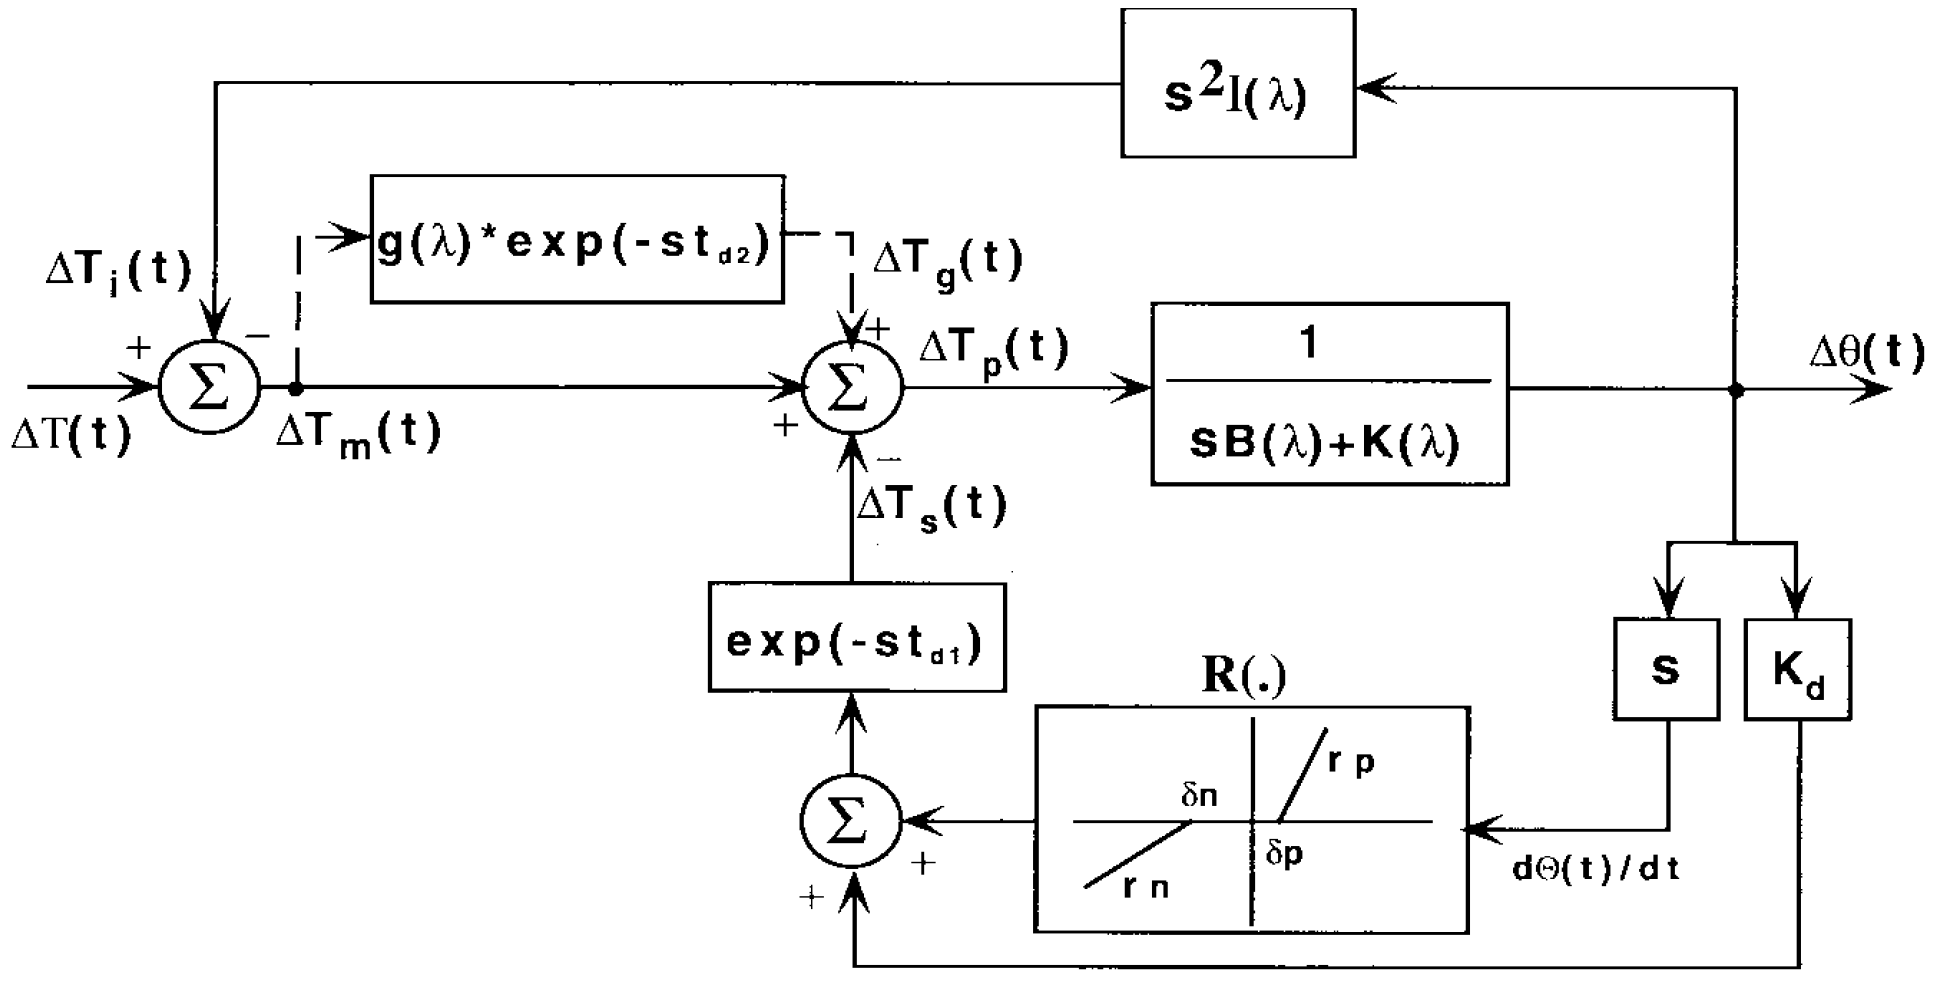
\includegraphics[width=\linewidth]{Figures/models_assumptions/model_zhang_1997.png}
    \caption{The model structure used by \citeauthor{zhang_simultaneous_1997}. System input $\Delta T(t)$ and output $\Delta \theta (t)$ are elbow joint torque and angle deviations respectively. The operating point is denoted by $\lambda$ (i.e. system state). $I(\lambda)$, $B(\lambda)$ and $K(\lambda)$ denote the intrinsic properties limb inertia, joint viscosity and stiffness respectively. The afferent feedback from GTO's is determined by gain $g(\lambda)$ with time delay $t_{d2}$, resulting in torque $\Delta T_g (t)$. The afferent feedback from the MS is separated in a position part with gain $K_d$ and velocity contribution via the asymmetric nonlinearity $R( \bullet )$, finally affected by time delay $t_{d1}$ to result in the torque $\Delta T_s (t)$. Figure adapted from \citet{zhang_simultaneous_1997}.}
    \label{fig:model_zhang_1997}
\end{figure}




\section{Limb muscle structure simplification -- lumping }
\citeauthor{zhang_simultaneous_1997} modelled the elbow joint \cite{zhang_simultaneous_1997} (see \autoref{fig:model_zhang_1997}), \citeauthor{van_der_helm_identification_2002} and \citeauthor{schouten_nmclab_2008} created a model to identify the shoulder dynamics from the wrist position \cite{van_der_helm_identification_2002, schouten_nmclab_2008} (see \autoref{fig:model_helm_2002} and \ref{fig:model_schouten_2008} respectively) and \citeauthor{mugge_rigorous_2010} modelled the ankle joint \cite{mugge_rigorous_2010}. All these studies lumped the agonist and antagonist muscles into one system. This simplification means that there are no moment arms used. The points of origin or insertion of the individual muscles were not estimated and hence no individual muscle forces were estimated. To account for this, only net joint torques are considered. 

A different approach proposed by \citeauthor{kearney_identification_1997} and later adapted by \citeauthor{mirbagheri_intrinsic_2000} consisted of only modelling the plantar flexor muscles to identify the ankle joint dynamics \cite{kearney_identification_1997, mirbagheri_intrinsic_2000} (see \autoref{fig:model_mirbagheri_2000}). The omission of the dorsiflexor muscles in the model was justified by keeping the experimental conditions such that the dorsiflexor muscles were not activated (validated by EMG measurements). If any activity was measured the data from that trial was discarded. The passive contributions of the dorsiflexor muscles were only apparent in the intrinsic pathway (discussed further in \autoref{sec:ass_intrinsic}). 

Another study by \citeauthor{de_gooijer-van_de_groep_estimation_2016} did use an antagonistic muscle structure, in which the wrist flexor and extensor muscle groups were modelled separately \cite{de_gooijer-van_de_groep_estimation_2016}. This structure required the inclusion of moment arms, which were modelled wrist angle dependent. Since the extensor group consisted of two separate muscles with different tendons (\textit{extensor carpi radialis longus} and \textit{brevis}) and only a combined EMG signal could be measured, the extensor moment arm was taken as the average of the two separate moment arms. 



\section{Muscle-tendon unit modelling}
% \tred[alternative title: measured data to muscle elongation (???)]
The muscle-tendon unit (MTU) is known to have quite complicated dynamics, and the tendon length relative to the muscle fibre length greatly influences the proportion of strain taken up by muscle and tendon \cite{zajac_muscle_1989}. Although these effects are known, many studies take the measured limb position or joint angle proportional to muscle elongation, implying an infinitely stiff tendon. Especially for compliant tendons (large tendon slack length with respect to  optimal muscle fibre length, e.g. Achilles tendon of plantar flexors) significant MTU interaction can lead to a distorted estimation of the force length curve \cite{zajac_muscle_1989}. 

\citeauthor{zhang_simultaneous_1997} acknowledged that the tendon in the MTU plays a significant role for abrupt change in muscle length, which they accounted by using small amplitude perturbations \cite{zhang_simultaneous_1997}. As a consequence, the joint angle was taken proportional to muscle elongation in the parameter estimation. \citeauthor{mirbagheri_intrinsic_2000} also took the ankle rotation proportional to the muscle elongation, i.e. not considering MTU dynamics, though abrupt changes in muscle length were present during their experiments \cite{mirbagheri_intrinsic_2000}. Similarly, \citeauthor{de_gooijer-van_de_groep_estimation_2016} took the wrist angle proportional to muscle elongation (corrected angle dependent moment arm), hence no MTU interaction was modelled \cite{de_gooijer-van_de_groep_estimation_2016}. 

In the study of \citeauthor{van_der_helm_identification_2002} the wrist position was taken proportional to muscle stretch, and tendon stretch was not considered. There was however a viscoelastic contact model considered to link the measured handle position to the hand position, representing the displacement of skin and movement of fingers \cite{van_der_helm_identification_2002}. This contact model was also employed by \citeauthor{schouten_nmclab_2008} for the wrist and \citeauthor{mugge_rigorous_2010} for the foot, to obtain the estimated wrist position and ankle angle respectively \cite{schouten_nmclab_2008,mugge_rigorous_2010}. These two studies did however consider separate muscle and tendon elongation. The force in tendon and muscle was assumed equal (connected in series), and consequently part of the joint translation or rotation was accounted by the tendon with estimated stiffness $k_\text{tendon}$. The muscle contractile element was represented by a linearized Hill model. 



% MIRBAGHERI
\begin{figure}[t]
    \centering
    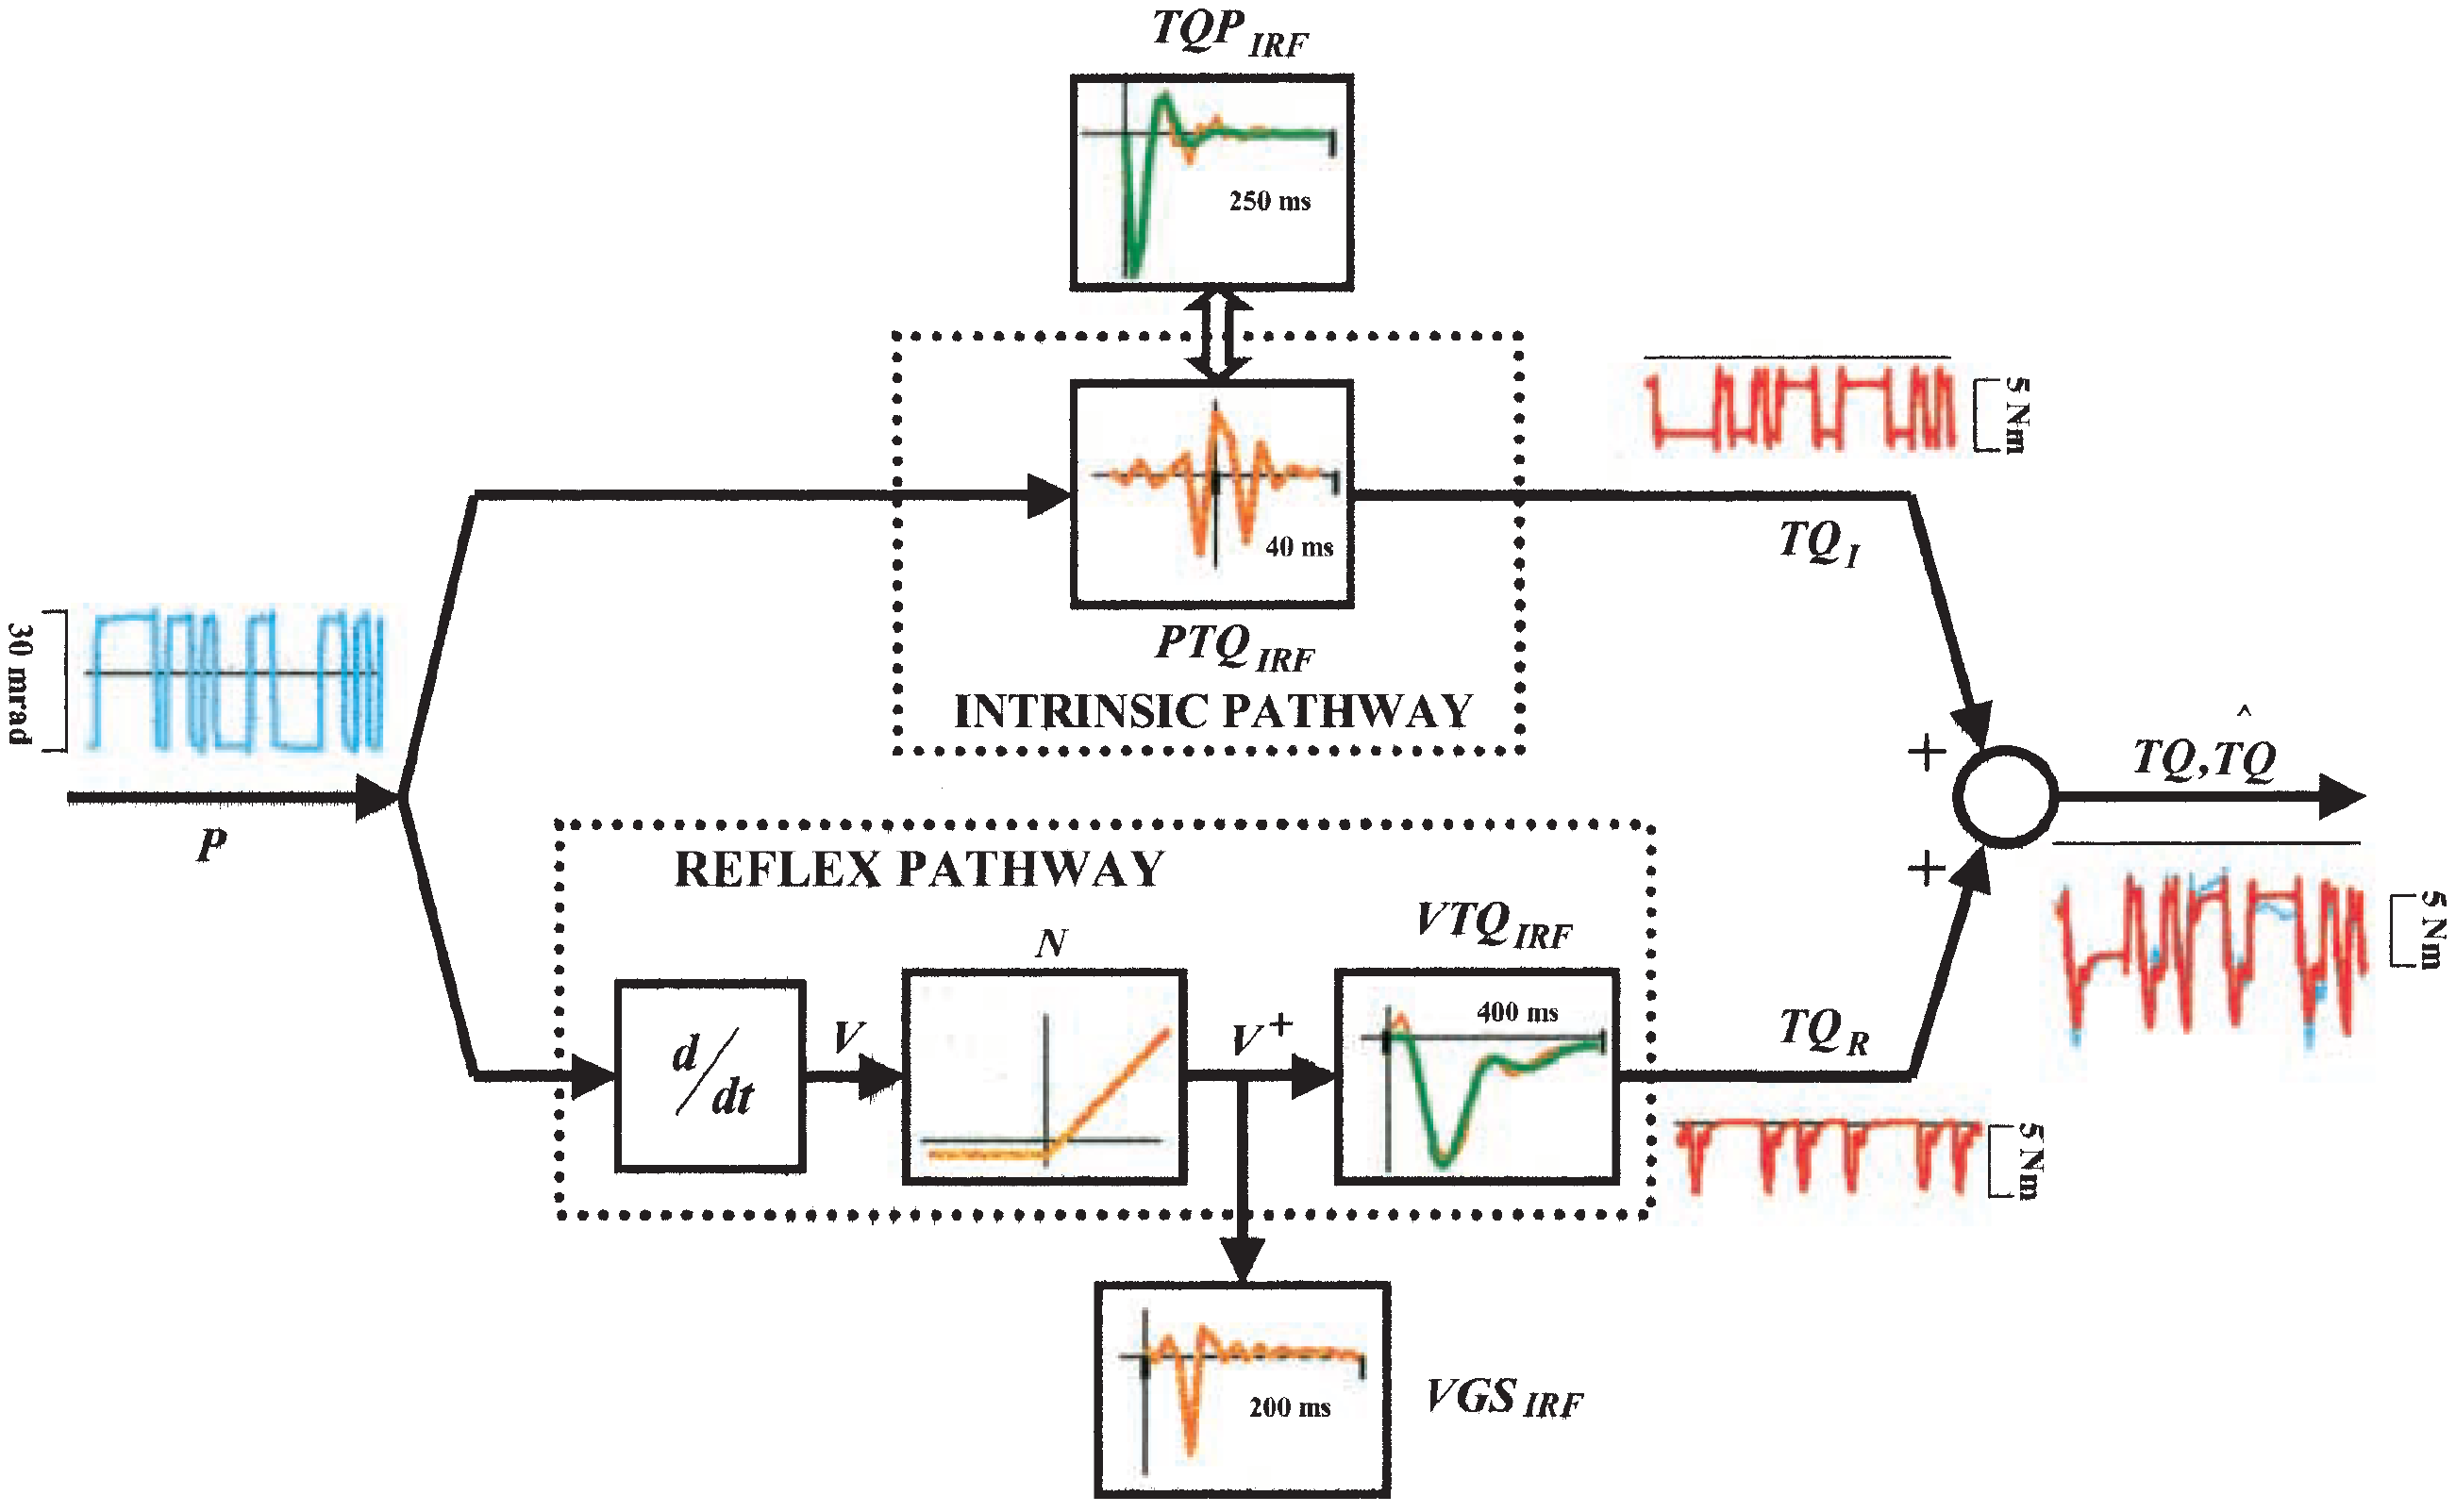
\includegraphics[width=\linewidth]{Figures/models_assumptions/model_mirbagheri_2000.png}
    \caption{Model structure of \citeauthor{mirbagheri_intrinsic_2000}, top pathway represents the intrinsic contribution, modelled by a second order spring-damper system with $I$, $B$ and $K$. The bottom pathway represents afferent feedback, only mediated by velocity feedback. The velocity is passed through a static nonlinearity $N$, closely resembled by a half-wave rectifier, resulting in only positive velocity $V^+$. This is used as activation signal for the reflex stiffness dynamics, $VTQ_{IRF}$, which comprises  a third order model with a time delay. Figure adapted from \citet{mirbagheri_intrinsic_2000}.}
    \label{fig:model_mirbagheri_2000}
\end{figure}



\section{Muscle activation dynamics}
\label{sec:muscle_act_dyn}
Upon application of an neural activation signal to the muscle, it takes some time for the muscle to buildup force, characterised by the muscle activation dynamics. In the considered studies different systems are used to describe these dynamics, though there is not as much variation as in the other aspects of the neuromuscular system. 

\citeauthor{zhang_simultaneous_1997} did not model any separate activation dynamics, but simplified this process by incorporating it in the modelled time delays for the afferent feedback (discussed further in \autoref{sec:ass_afferent}) \cite{zhang_simultaneous_1997}. In \citeauthor{van_der_helm_identification_2002}, the activation dynamics were modelled as a first order low-pass filter \cite{van_der_helm_identification_2002}. 

A more frequently used representation of the activation dynamics is a second order low-pass filter \cite{schouten_nmclab_2008, mugge_rigorous_2010}. \citeauthor{mirbagheri_intrinsic_2000} also used second order low-pass activation dynamics, but did not find a good fit in previous work, and therefore included a first order pole in the model \cite{mirbagheri_intrinsic_2000, mirbagheri_parametric_1995}. The entire model by \citeauthor{mirbagheri_intrinsic_2000} was similar to the model structure proposed by \citeauthor{kearney_identification_1997}, except for this additional pole. In general, it is assumed that the activation dynamics only affect the afferent feedback path, since the intrinsic properties are assumed constant and instantaneous during trials (see \autoref{sec:ass_intrinsic}). 

The model of \citeauthor{de_gooijer-van_de_groep_estimation_2016} also employed second order filter activation dynamics and used it to relate measured EMG activity to the active state of the muscle \cite{de_gooijer-van_de_groep_estimation_2016}. The active state (in combination with muscle length and velocity) was used to determine the force in the muscle using a Hill-type muscle model. 


% HELM
\begin{figure}[t]
    \centering
    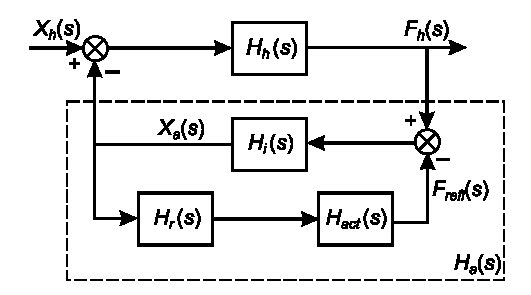
\includegraphics[width=0.6\linewidth]{Figures/models_assumptions/model_helm_2002.pdf}
    \caption{Linear model used by \citeauthor{van_der_helm_identification_2002}, the handle position $X_h(s)$ is the input of the model. From the difference in handle position and arm position, the handle force $F_h(s)$ is estimated (model output), by means of a viscoelastic hand-grip contact model $H_h(s)$. This handle force is used to determine the arm position $X_a(s)$. The arm position is then used to determine the reflexive contribution via $H_r(s)$, which comprises MS position and velocity feedback and a time delay. The reflexive contribution is then affected by the muscle activation dynamics $H_\text{act}(s)$ (first order low-pass filter), to result in the reflexive force contribution $F_\text{refl}(s)$. Figure adapted from \citet{van_der_helm_identification_2002}.}
    \label{fig:model_helm_2002}
\end{figure}




\section{Afferent feedback} \label{sec:ass_afferent}
Afferent feedback (also referred to as reflexive feedback) is considered as the muscle activity that results from feedback of the sensory organs in the muscles. In comparison to assumptions made in other aspects of the system identification (which for the most part can be considered as simplifications for parameter estimation), the modelling of the afferent feedback is mostly influenced by the fact that there is no consensus about the origin of the different observed reflexes. Afferent feedback is considered energy efficient, since it only provokes muscle activity in response to a perturbation. 

The two known receptor organs described in physiological studies are the muscle spindles (MS) and Golgi tendon organs (GTO). The muscle spindles are located in the muscle belly, parallel to the muscle fibres and are presumed to be sensitive to fibre stretch (also referred to as position) and velocity. It is believed that both the fibre stretch and velocity information is transmitted through the Ia afferent nerve fibre to the $\alpha$-motoneuron, and only the fibre stretch through the II afferent nerve fibre. Two efferent $\gamma$ neurons are believed to set the sensitivity of the MS, one dynamic mostly influencing the sensitivity of the Ia afferent, and one static mostly influencing the II afferent \cite{mileusnic_mathematical_2006}. Furthermore, it is believed that the muscle spindle has an asymmetric response, with the Ia afferent mostly sensitive to eccentric velocity, and the II afferent mainly sensitive to elongation with respec to the resting length \cite{burke_muscle_1978}. 

The other receptor, the Golgi tendon organ, is located exclusively at the muscle-tendon or muscle-aponeu- rosis junction \cite{jami_golgi_1992}, hence in series with the muscle fibres. When the MTU elongates, the GTOs are compressed, and they will start firing through the afferent Ib nerve fibre. The stretch in the tendon is a measure for the force in the muscle, since muscle and tendon are in series. It is shown however that the GTO is more sensitive to active muscle contraction than to passive muscle stretch \cite{houk_responses_1967}.

In the model by \citeauthor{de_gooijer-van_de_groep_estimation_2016} no proprioceptors were modelled, thus no attempt was made identify the origin of the reflex activity since it was out of their scope \cite{de_gooijer-van_de_groep_estimation_2016}. The model was a variation on the model of \citeauthor{de_vlugt_relation_2010}, where it was explained that the modelling of proprioception was not required since EMG activity was used directly to estimate the muscle torques \cite{de_vlugt_relation_2010}. Because of the used ramp and hold (RaH) perturbations in combination with the task description to completely relax, it was expected that only reflexive activity was evoked. The absence of voluntary contractions in the EMG signal could not be validated. 


% MS feedback has been described as asymmetric \cite{terjung_neural_2011} 
% The modelling of afferent feedback varies the most across the considered studies, and the underlying mechanism is 

\subsection{Receptor modelling}
The modelling of the two receptors varies a lot between the studies (see overview in \autoref{tab:overview_assumptions}, column afferent feedback). \citeauthor{mirbagheri_intrinsic_2000} considered only velocity feedback, presumably arising from MS feedback though not explicitly written \cite{mirbagheri_intrinsic_2000}. The measured angle was differentiated and the resulting angular velocity of the ankle was provided to a static nonlinear element, a half wave rectifier. As a consequence, reflexive feedback was only evoked by eccentric velocity of the plantar flexor muscles, corresponding to the unidirectional sensitivity of the stretch reflex \cite{kearney_system_1983}. The output of the nonlinearity was normalised, and thus only corresponds to the activation caused by the velocity. No muscle fibre length or muscle force feedback was considered. The model used by \citeauthor{mirbagheri_intrinsic_2000} was first introduced by \citeauthor{kearney_identification_1997}, and slightly adapted, but the receptor modelling remained unchanged. 
% \tred[discuss gain IRF? or in integration] 

Initially, \citeauthor{zhang_simultaneous_1997} did model both MS and GTO feedback. The MS feedback was separated in a velocity and position component, of which the former was modelled by two half-wave rectifiers (one for concentric and one for eccentric muscle velocity) \cite{zhang_simultaneous_1997}. These were modelled asymmetrically, since the response of the MS to positive and negative velocity was assumed different \cite{houk_neural_1981}. Each side of the half-wave rectifiers was specified by a slope and a threshold, resulting in an asymmetric dead-zone. The MS position feedback was taken as a simple gain, hence not asymmetric. In the initial model force (GTO) feedback was incorporated, also represented by a gain. However, in a simplified version of the model for the parameter estimation, GTO feedback was omitted, as well as the dead-zone for the velocity feedback. %All parameters were taken dependent on the operating state, among which the mean joint angle, mean background torque and perturbation properties. 

The model of \citeauthor{van_der_helm_identification_2002} included position and velocity feedback, representing MS feedback, but no force feedback was used in the model \cite{van_der_helm_identification_2002}. It was later mentioned that the inclusion of force feedback in the model yielded very small force reflex gains or bad convergence of the model, which the authors ascribed to negligible force feedback under the presented experimental conditions. The position and velocity feedback were described by separate gains, $k_p$ and $k_v$ respectively. 

The model introduced by \citeauthor{schouten_nmclab_2008} was \tred[the first] to incorporate both GTO and MS feedback and estimate these parameters \cite{schouten_nmclab_2008}. GTO feedback was modelled as a gain $k_f$, and was activated by the estimated force in the MTU. Since GTO feedback is mostly associated with inhibitory effects, a positive gain was considered inhibitory and a negative gain excitatory. The MS feedback was similar to \citeauthor{van_der_helm_identification_2002} modelled by gains for the position, $k_p$, and velocity, $k_v$. For the MS, positive gains were associated with excitatory effects, and negative with inhibitory. In addition, since some studies suggested the MS was also sensitive to fibre acceleration, an additional acceleration gain, $k_a$, was modelled. However this gain was later set to zero without explanation. The study by \citeauthor{mugge_rigorous_2010} used the same model as \citeauthor{schouten_nmclab_2008}, but removed the acceleration gain \cite{mugge_rigorous_2010}.

In all studies where MS feedback consisted of both position and velocity feedback, these were separated completely, unlike the presumed underlying physiology where the Ia afferent is believed to be sensitive to both and the II afferent to merely position \cite{van_der_helm_identification_2002, schouten_nmclab_2008, mugge_rigorous_2010}. Furthermore, although the unidirectional (nonlinear) properties of the MS were acknowledged in these studies, these were not modelled. The used structure, flexor and extensor lumped, did not allow for this. But as a result the inhibitory and excitatory effects of MS feedback are equal in size for equal valued $k_p$ and $k_v$ with different signs. This is not in correspondence with reality, where the flexor and extensor muscles often cannot deliver an equal amount of force (see e.g. \cite{winters_analysis_1985}). 


% SCHOUTEN
\begin{figure}[t]
    \centering
    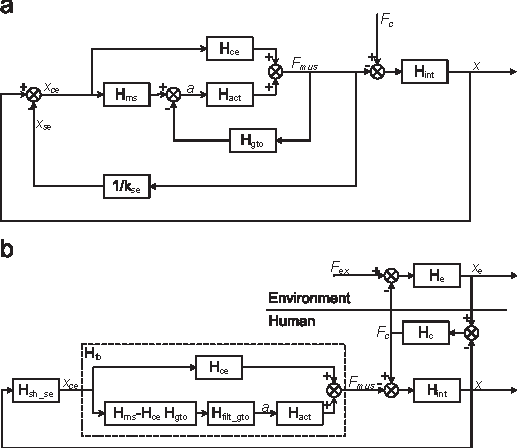
\includegraphics[width=.8\linewidth]{Figures/models_assumptions/model_schouten_2008.pdf}
    \caption{Model structure used by \citeauthor{schouten_nmclab_2008} to identify shoulder joint dynamics. \textbf{(a):} Intrinsic dynamics due to tonic contraction are described in $H_\text{ce}$. Parallel to this, the reflexive contribution is obtained from the MS feedback ($H_\text{ms}$) excited by length ($x_\text{ce}$) and lengthening velocity and GTO feedback ($H_\text{gto}$) excited by muscle force $F_\text{mus}$. \textbf{(b):} Human in combination with the environment, including contact ($H_\text{c}$) and robotic manipulator dynamics ($H_\text{e}$). The difference in contact and muscle force determine the force affected by the inertia ($H_\text{int}$) of the limb. The model structure used by \citet{mugge_rigorous_2010} was very similar, with some differences in additional external signals (e.g. neural activation additional to voluntary co-contraction). Figure adapted from \citet{schouten_nmclab_2008}. }
  \label{fig:model_schouten_2008}
\end{figure}


% SCHOUTEN AND MUGGE
% \begin{figure}[t]
% % \centering
% \begin{minipage}[t]{.53\textwidth}
%   \centering
%   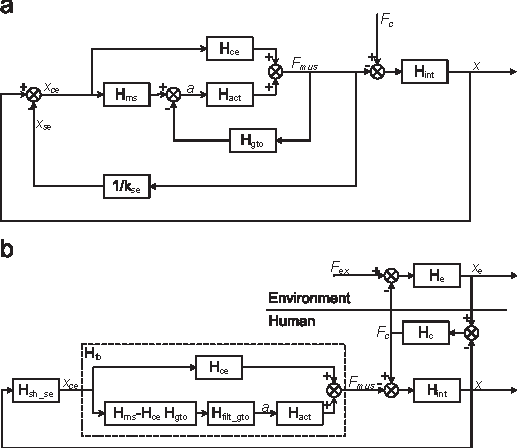
\includegraphics[width=\linewidth]{Figures/models_assumptions/model_schouten_2008.pdf}
%   \captionof{figure}{Model structure used by \citeauthor{schouten_nmclab_2008} to identify shoulder joint dynamics. \textbf{(a):} Intrinsic dynamics due to tonic contraction are described in $H_\text{ce}$. Parallel to this, the reflexive contribution is obtained from the MS feedback ($H_\text{ms}$) excited by length ($x_\text{ce}$) and theningleng velocity and GTO feedback ($H_\text{gto}$) excited by muscle force $F_\text{mus}$. \textbf{(b):} Human in combination with the environment, including contact ($H_\text{c}$) and robotic manipulator dynamics ($H_\text{e}$). The difference in contact and muscle force determine the force affected by the inertia ($H_\text{int}$) of the limb. Figure adapted from \citet{schouten_nmclab_2008}. }
%   \label{fig:model_schouten_2008}
% \end{minipage} $\quad$
% \begin{minipage}[t]{.43\textwidth}
%   \centering
%     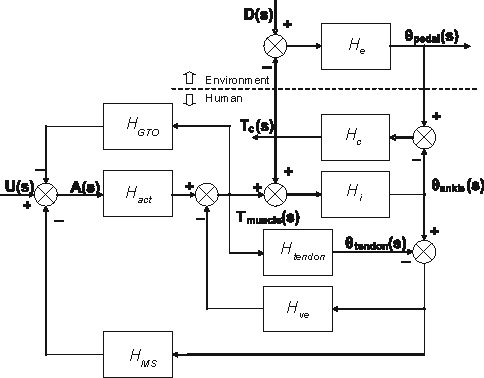
\includegraphics[width=\linewidth]{Figures/models_assumptions/model_mugge_2010.pdf}
%     \caption{Model structure used by \citeauthor{mugge_rigorous_2010}, derived from \cite{schouten_nmclab_2008}.  Figure adapted from \citet{mugge_rigorous_2010}.}
%     \label{fig:model_mugge_2010}
% \end{minipage}
% \end{figure}


% \begin{figure}[t]
%     \centering
%     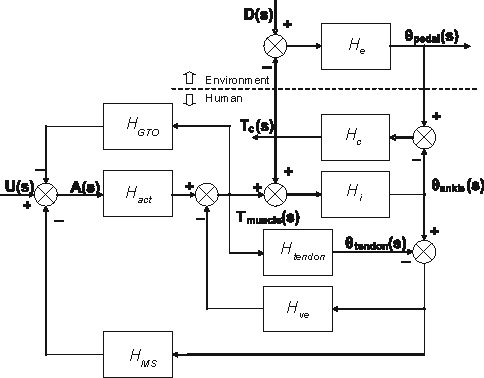
\includegraphics[width=\linewidth]{Figures/models_assumptions/model_mugge_2010.pdf}
%     \caption{Model structure used by \citeauthor{mugge_rigorous_2010}, derived from \cite{schouten_nmclab_2008}. Figure adapted from \citet{mugge_rigorous_2010}.}
%   \label{fig:model_mugge_2010}
% \end{figure}



\subsection{Time delays}
\label{sec:ass_afferent_delay}
Afferent feedback has a substantial time delay from detection of the receptor organs to muscle action, caused by travel time from the receptors to the motoneurons via the afferent nerve fibre, processing of the detected changes and travel time of the motor command via the efferent nerve fibre. The neural travel time limits the ability of reflexive feedback to be effective for high frequency perturbations. The modelling of the delays shows some variation across the considered studies. In all studies the afferent, processing and efferent delays are lumped into one for simplicity, but the variation lies in the separation of MS and GTO feedback delay.

\citeauthor{zhang_simultaneous_1997} modelled the GTO and MS delay as separate two variables \cite{zhang_simultaneous_1997}. Although the GTO feedback was later omitted, it was assumed that the GTO delay was larger due to the involvement of interneurons. To estimate the time delay for MS feedback, a tendon tapping experiment was performed separately. The modelled time delay included the muscle activation dynamics (as discussed in \autoref{sec:muscle_act_dyn}), and thus the delay was taken as the time between the moment of tendon tapping and the onset of reflex torque. \citeauthor{mirbagheri_intrinsic_2000} and \citeauthor{van_der_helm_identification_2002} did not consider GTO delay, hence the modelled delay only represents MS delay \cite{mirbagheri_intrinsic_2000, van_der_helm_identification_2002}. \citeauthor{schouten_nmclab_2008} used the same value for the time delay for both GTO and MS feedback \cite{schouten_nmclab_2008}. Dynamics of the $\alpha$-motoneuron pool at the spinal cord, integrating all the afferent feedback, were assumed much faster than the other dynamics in the loop, and was not modelled individually. \citeauthor{mugge_rigorous_2010} used mostly the same model, but made a slight variation in the time delays by considering separate parameters for GTO and MS feedback \cite{mugge_rigorous_2010}. The reported parameter for MS delay was longer than GTO delay, contradicting the assumption of \citeauthor{zhang_simultaneous_1997}. 

All these modelled time delays are only able to capture the short-latency reflex (SLR), which is a monosynaptic reflex. Other more coordinated reflexes as the medium- and long-latency reflex (MLR and LLR respectively), presumably more spinal levels are involved, hence longer neural travel time and longer integration time. This makes it a lot harder to model, involves a lot more uncertainty, and therefore these longer latency reflexes are often omitted for simplification of the models. \citeauthor{mugge_rigorous_2010} did try to substitute the SLR for the LLR by changing the boundaries for the delay parameters in the parameter estimation \cite{mugge_rigorous_2010}. This yielded worse fits compared to the SLR boundaries. In reality, presumably a combination of SLR, MLR and LLR is present, but there have been no attempts to incorporate this combination in parametric system identification studies. 

\subsection{Sensitivity to afferent feedback}
In the central nervous system (CNS), there are mechanisms to set the sensitivity of the muscle spindles, allowing the CNS to change the reflex response to detected length and velocity information. According to the `fusimotor set' hypothesis, this is is done through two efferents from the $\gamma$-motoneurons, the static and dynamic efferents ($\gamma_s$ and $\gamma_d$ respectively) \cite{prochazka_fusimotor_1985}. These are assumed to set the sensitivity of the Ia and II afferents independently, and are set consistently for certain types of movements. A similar mechanism to adapt the sensitivity for force feedback (Ib afferent) does not exist. Moreover, a static and linear relation between muscle force and afferent activity is found \cite{crago_sampling_1982}. The mechanism to change the sensitivity to muscle force feedback are set in the CNS, e.g. presynaptic inhibition, by changing the sensitivity of the Ib afferent receiving neuron. This shows that the CNS has many mechanisms to change the sensitivity of the different types of afferent feedback and thus modulate the $\alpha$-motoneuron activity. 

The gains for the afferent feedback in the considered studies were all modelled constant for each presented condition. The $\gamma_s$ and $\gamma_d$ were assumed constant per task type in \cite{van_der_helm_identification_2002, schouten_nmclab_2008, mugge_rigorous_2010}, resulting in static $k_p$ and $k_v$ gains, per task movement type. If force feedback was modelled this was also modelled by a constant gain, again dependent on the type of movement. The type of movement was controlled by specifying a tasks, and varying the bandwidth of the presented perturbations. Hence, for each condition the different parameters were estimated. The other studies also took the gains for the modelled reflexive feedback constant during a movement type, but estimated it dependent on  e.g. the presented background torque, joint configuration and perturbation properties \cite{zhang_simultaneous_1997, mirbagheri_intrinsic_2000}. 

% Gains afferent feedback
% All studies including afferent feedback organs (Helm, Schouten, Mugge, …) : Gamma static and dynamic and GTO gain modelled constant (time invariant), only dependent on task. 
% Mirbagheri et al 2000; determined IRFs per condition, and in condition constant can be compared to constant gain per condition
% Zhang Rymer 1997; same, nonlinearity parameters (slope + and -) and pos gain determined per background torque. (~ time invariant for task) 


\section{Linear versus nonlinear}
Although it is known that the human body behaves highly nonlinear, many studies used linear modelling techniques \cite{van_der_helm_identification_2002, schouten_nmclab_2008, mugge_rigorous_2010}. As a consequence, small perturbation signals have to be used, to disturb the system near the operating point that is being identified. When large amplitude (or high velocity) perturbations are applied, the nonlinearities in the system are excited, and the linear model will not be able to explain the measured output of the signal. \citeauthor{schouten_nmclab_2008} and \citeauthor{mugge_rigorous_2010} employed a Hill model for the dependency of muscle length and velocity on the muscle force, which had to be linearized first \cite{schouten_nmclab_2008, mugge_rigorous_2010}.

%\citeauthor{zhang_simultaneous_1997} and \citeauthor{mirbagheri_intrinsic_2000}
The studies that did include nonlinearities in their model (for the MS feedback) still used low amplitude perturbation signals (\citeauthor{zhang_simultaneous_1997} standard deviation on amplitude 1.5 deg \cite{zhang_simultaneous_1997}, \citeauthor{mirbagheri_intrinsic_2000} amplitude jumps of approx. 1.7 deg \cite{mirbagheri_intrinsic_2000}). The used perturbation signal is typically continuous, having frequency content equally distributed across a specified bandwidth \cite{zhang_simultaneous_1997, van_der_helm_identification_2002, schouten_nmclab_2008, mugge_sensory_2009}. In contrast, \citeauthor{mirbagheri_intrinsic_2000} used pseudorandom binary sequence (PRBS) signals, jumping at random time instances to another peak value. In these sequences, the maximum velocity in the ankle was approx. 11 deg/s \cite{mirbagheri_intrinsic_2000}. A clear difference in the PRBS trials compared to continuous trials, is that in PRBS the velocity distribution is a lot smaller, while still exiting a broad frequency range. On the other hand, the power at the different frequencies is not as equally distributed as in continuous perturbation signals. 

The ramp and hold (RaH) perturbations used by \citeauthor{de_gooijer-van_de_groep_estimation_2016} were high in amplitude, i.e. over the full range of motion (RoM) of the wrist joint. Furthermore, the movement over the complete RoM was imposed in \SI{1}{\second}, resulting in high angular velocities. Therefore, a nonlinear model was used to capture the nonlinear joint physiology. Forces were estimated with nonlinear force-length and force-velocity curves (adapted from \cite{thelen_adjustment_2003}), and the force in the muscle parallel elastic element was nonlinear. 



% XXX
% \section{Time variant versus time invariant}

% \subsection{EMG proportional to muscle force}

% \subsection{Muscle thixotropy}
% XXX




\section{Intrinsic feedback} \label{sec:ass_intrinsic}
Intrinsic properties are considered as the the mechanical properties of the joint, passive tissue, and active muscle fibres. The main source of intrinsic feedback is seen as the viscoelastic properties of the muscles, determined by the force-length and force-velocity characteristics of the muscle \cite{winter_biomechanics_1988}. The viscoelastic properties can be increased by muscle co-contraction. The major difference between intrinsic and reflexive feedback is that intrinsic feedback is instantaneous, where reflexive feedback is characterised by delays (as discussed in \autoref{sec:ass_afferent_delay}). The instantaneous property of intrinsic feedback makes it very effective for rejecting perturbations at higher frequencies, at cost of greater energy consumption due to the need for a high degree of muscle co-contraction. The modelling of intrinsic feedback shows some variation. 

% 
\citeauthor{zhang_simultaneous_1997} described the intrinsic feedback by a second order spring-damper system, where the inertia included the contribution of the limb and a wrist attachment \cite{zhang_simultaneous_1997}. A separate experiment to estimate the inertia was performed, in which the subjects were asked to fully relax their arm during perturbation. The stiffness $k$ and damping $b$ were taken dependent on the operating point.
 
\citeauthor{mirbagheri_intrinsic_2000} also modelled the intrinsic properties as a second order spring-damper model, completely parallel to the afferent feedback \cite{mirbagheri_intrinsic_2000}. The stiffness $k$ and damping $b$ describe the dynamic viscoelastic properties of the muscle, and the inertia $I$ the static properties of both the limb and boot worn during the experiment. Since the intrinsic pathway was completely parallel to the afferent path, the reflexive forces were not affected by the inertia of the limb and boot. However, due to the model parametrisation, the effects of inertia on reflexive feedback could be hidden in some of the parameters describing the activation dynamics (not all parameters have a direct physiological meaning). To make sure that the intrinsic properties were not contaminated by reflex effects, the length of the IRF representing intrinsic feedback was constrained to be less than the delay associated with afferent feedback, ca. \SI{40}{\milli\second}. 

In the model of \citeauthor{van_der_helm_identification_2002}, the intrinsic properties were also described by a second order spring-damper system \cite{van_der_helm_identification_2002}. No separate parallel pathway for intrinsic feedback exists, hence reflexive feedback is affected by the stiffness, damping (viscosity) and inertia of the joint. The stiffness and damping parameters increase with the level of (co-)contraction. 

\citeauthor{schouten_nmclab_2008} and \citeauthor{mugge_rigorous_2010} take inertia of the limb separate, and model no separate passive viscoelastic properties of the joint \cite{schouten_nmclab_2008, mugge_rigorous_2010}. The active viscoelastic intrinsic properties ($k$ and $b$) due to (co-)contraction (tonic contraction) are modelled parallel to the afferent feedback, not affected by the activation dynamics (i.e. instantaneous force) and dependent on both the operating point and task type of a trial. The resulting intrinsic contribution (tonic) is then summed with the afferent contribution (phasic), and the sum of both is affected by the inertia of the limb.

Since the RaH perturbations used by \citeauthor{de_gooijer-van_de_groep_estimation_2016} were assumed to only evoke reflexive activity, the intrinsic properties were not affected by voluntary (co-)contraction \cite{de_gooijer-van_de_groep_estimation_2016}. The intrinsic contribution to movement was modelled by the passive elastic element parallel to the contractile element in the Hill-type muscle model. The elastic element possibly also contained contribution from the tendon stiffness and joint resistance. This elastic force was assumed to decrease, due to relaxation in the muscle connective tissue, modelled by a first order filter. This was previously modelled by \citeauthor{de_vlugt_relation_2010} as a viscous damper, more similar to the other studies \cite{de_vlugt_relation_2010}. Inertia was also estimated, consisting of the wrist, hand and manipulator handle. 

In none of the studies additional supra spinal commands were considered. The supra spinal commands were assumed constant depending on task type, and were modelled by viscoelastic parameters of the active co-contracted muscles. The level of co-contraction was taken movement type (or task) dependent in all the studies, and hence the stiffness and viscosity parameters were taken constant during the trials. The inertia was in some studies taken condition independent, and thus could be kept constant during the parameter estimation \cite{zhang_simultaneous_1997, van_der_helm_identification_2002, mugge_sensory_2009}.


% \subsection{viscoelasticity parameters independent}
In all studies, the intrinsic viscoelastic parameters (stiffness $k$ and viscosity $b$) were estimated independent. However, in reality there is significant parameter interplay, due to the underlying physiological mechanisms. This relation has been described by using e.g. a Voigt model, and the viscoelastic properties have been estimated using shear wave spectroscopy \cite{gennisson_viscoelastic_2010}. 
% XXX

% \subsection{Short range stiffness}








% ===========================================================================
\section{Implication of assumptions}
% NOTE: all assumptions are closelty interconnected, hence a clear separation is hard to do. Two main assumptions to which the others are closely related will be discussed, and the implications thereof. 
The preceding sections show that there is a wide variety in modelling of the neuromuscular system across the studies, based on various assumptions. An overview is presented in \autoref{tab:overview_assumptions}. The wide variety in modelling approaches shows that not all studies have the same goal. Where \cite{kearney_identification_1997, mirbagheri_intrinsic_2000, de_gooijer-van_de_groep_estimation_2016, jalaleddini_subspace_2017} used a model with as little as possible \textit{a priori} knowledge, other studies attempted to build (simplified) models based on the current believes about the human physiology involved with reflexes and movement \cite{zhang_simultaneous_1997, van_der_helm_identification_2002, schouten_nmclab_2008, mugge_rigorous_2010}. The former can be seen as more phenomenological studies, which can be used to determine characteristic differences between populations, but are not as informative as the latter, where the goal is to improve the understanding of the underlying physiology and relate changes in the physiologic state to the observed behaviour. Hence, the various identified assumptions all lead to some implications for system identification of the joint dynamics, and have a great influence on what exactly can be learned from the experiment and model. Since the assumptions and their implications are for the most part closely related, these cannot be clearly separated. Therefore, the implications will be discussed based on two main assumptions, relating to muscle-tendon interaction and lumping of muscles. 


\subsection{Muscle-tendon interaction}
A number of system identification studies did not consider muscle-tendon interaction, and consequently related joint ankle or position directly to muscle elongation \cite{zhang_simultaneous_1997, kearney_identification_1997, mirbagheri_intrinsic_2000, van_der_helm_identification_2002, de_gooijer-van_de_groep_estimation_2016}. When it is assumed that no MTU interaction occurs, this directly implies an infinitely stiff tendon. Especially for compliant tendons, such as the Achilles tendon connected to the plantar flexors in the lower leg, significant MTU interaction can be expected, which can lead to a distorted estimation of the muscle elongation. %This has consequences for the separation of intrinsic and reflexive contributions to the movement. 

As a consequence of omitting MTU interaction, intrinsic and reflexive contributions to movement cannot be accurately estimated.  
%Not considering MTU interaction can lead to a distorted estimation of muscle elongation and subsequently distortion in the estimated contribution of intrinsic properties to movement. 
In general, a simple spring-damper system consisting of two parameters is used to describe the intrinsic properties of all muscles, passive tissue, tendons and higher order joint resistance. Since these components do not all displace the same amount due to MTU interaction and different moment arms, the estimation of intrinsic properties is distorted (further discussed in \autoref{sec:rem_lumping-muscle}). 

Likewise, the distorted estimation of muscle elongation has implications on the degree of proprioceptive afferent activity leading to modulation of reflexes. The muscle spindles are sensitive to muscle elongation and lengthening velocity, which in case of an infinitely stiff tendon would be overestimated, since all the elongation is ascribed to the muscle. Some studies considered either position or velocity feedback, which has proven to result in models with reasonable \textit{variance accounted for} (VAF), but presumably leads to further overestimation of a single component to reflex modulation \cite{maas_is_2009}. Furthermore, all of the studies that did not model muscle-tendon interaction also omitted the Golgi tendon organ (i.e. force) afferent feedback. Omission of force feedback can further lead to overestimation of the modelled reflexive mechanism. The choice of proprioceptive receptor modelling does not seem to have a large influence on the prediction capabilities of the model (in terms of VAF), but do not necessarily resemble the physiology behind reflex modulation. 
% point about tendon in series, stiffness lot higher than muscle in passive state, hence due to 1/keq = 1/k1 + 1/k2 minor contribution. However, for fast movements, this is not the case.

Especially the omission of GTO force feedback contradicts findings reported by the group of Sinkjaer. Af Klint et al. found strong support for contribution of GTO feedback in addition to MS feedback in adaptations to ground irregularities during locomotion \cite{klint_afferent_2009}. However, the effect of GTO and MS feedback during locomotion appeared to be stance phase dependent, where respectively mid-stance MS feedback and late-stance GTO feedback was thought to be dominant \cite{grey_positive_2007, af_klint_sudden_2009}. This emphasises the need for additional measurement data, enabling further isolation of afferent activity during other motor tasks (i.e. balance, force, position tasks). 

% \tred[expected GTO feedback? Sinkjaer, af Klint??] \textcolor{red}{\lipsum[1]}
% - when not considered, GTO omitted. no physiological basis refl modulation
%     - expected role is substantial (sinkjaer, klint... ??)
% - Wrong estimation leads to wrong activation signal when considering afferent feedback


\subsection{Lumping muscle structure}
\label{sec:rem_lumping-muscle}
A very common simplification of the neuromuscular model is lumping of antagonistic muscle groups \cite{zhang_simultaneous_1997, van_der_helm_identification_2002, schouten_nmclab_2008, mugge_rigorous_2010}. This has as advantage that the model can be defined by less parameters compared to an antagonistic model (e.g. \cite{de_gooijer-van_de_groep_estimation_2016}). No moment arms for MTUs have to be estimated or averaged over multiple MTUs for the same function (i.e. flexion versus extension). Furthermore, the intrinsic properties (i.e. inertia, stiffness and damping) of limb, joint resistance, tendon, passive and active muscle tissue can all be lumped into a minimum of three parameters. The lumping of muscle groups with different function does however also have disadvantages when the intrinsic and reflexive effects on movements are under analysis. 

% - afferent inhibity/excit contribution. Goal is to separate how the reflexive contribition is build up. with this lumping, Ia, Ib and II afferents of muscle groups contribution to modulation cannot be determined. physiology behind this remains elusive. 
Firstly, due to lumping the afferent GTO and MS feedback from muscle groups with different functions cannot be well separated. However, the different muscle groups are always making opposite movements, so the afferent signals are expected to be opposite. To get a better understanding of reflex modulation, a separation of the afferent signals form the different groups is required, which means that the flexors and extensors have to be lumped separately. In simulation studies (e.g. \cite{mugge_modeling_2012}) this separation is relatively straightforward, but the large number of additional parameters make this approach impractical for identification studies. Although the study of \citeauthor{de_gooijer-van_de_groep_estimation_2016} did use an antagonistic model \cite{de_gooijer-van_de_groep_estimation_2016}, fitting the model might only be possible under specific experimental conditions. This hampers the use of such an antagonistic model in system identification experiments were wide bandwidth perturbation signals are used (further discussed in \autoref{sec:rem_incompatibility}).

% - nonlinear properties proprioceptors only under specific conditions. 
Secondly, the nonlinear properties of the proprioceptors cannot accurately be modelled and identified with a fully lumped muscle model. The muscle spindles are only sensitive to muscle lengthening and Golgi tendon organs are mostly sensitive to active muscle force. For GTO force feedback a simple gain with a time delay is typically used \cite{schouten_nmclab_2008, mugge_rigorous_2010}. Apart from the nonlinearity of the GTO itself, the flexor and extensor muscles often have asymmetric force characteristics (e.g. plantar flexors stronger than dorsiflexors \cite{fukunaga_specific_1996}). Consequently, modelling the GTOs in plantar flexor and dorsiflexor muscles with a single linear gain could result in an overestimation of plantar flexor MTU force contribution to the afferent signal. The lumping in combination with no MTU interaction has as a consequence that the source of the afferent activity per muscle group can never be found. 

% - intrinsic estimated properties do not resemble underlying physoilogy, but contaminated. This does not imply that this is incorrect, but applying new tech UUS that provides specific quantitative data about specific (sub)module creates mismatch. 
Lastly, the lumping of intrinsic parameters makes the system identification and parameter estimation easier, but does not result in parameters that have a direct physiological meaning. Furthermore, the parameters that are defined, possibly do not only contain contributions of the modelled structure, but are contaminated by contributions of other tissue, e.g. joint resistance. This is not wrong on its own, but has consequences for the usefulness of additional measurement data that has a direct physiological basis (e.g. viscoelastic properties of tendon and muscle). This incompatibility of data and current models will be further discussed in \autoref{sec:rem_incompatibility}. 

% - separation of muscle groups is not that straightforward. apart from more parameters in current model doubled, muscle model, more parameters due to introduction of moment arms, more tendon, joint friction for example not as easily lumped. A view on what these implications mean for the neuromuscular model is presented in last section. 



% \subsection{Overview implications and what ultrasound can mean}
% Relate assumptions to goals? 
% table goals, and which technology can fulfil them. 

\iffalse

	\subsection{Required measurement for relaxing assumptions}
	To relax the listed assumptions, some 
	
\fi







% TABLE OVERVIEW
\begin{landscape}


%\newcolumntype{Y}[1]{>{\footnotesize \hangindent=1em \raggedright \let\newline\\\arraybackslash}p{#1}}
\newcolumntype{Y}[1]{%
	>{\footnotesize\everypar{\hangindent=1em}\arraybackslash}p{#1}%
}
\renewcommand{\arraystretch}{1.2}
\newcommand{\customnewline}{\par}
% INSERT IN NEW TABLE
% \begin{tabular}{Y{7em}Y{5em}Y{10em}Y{10em}Y{10em}Y{10em}Y{10em}}
% \normalsize\textbf{Study}  & \normalsize\textbf{Joint}  & \normalsize\textbf{Limb structure} & \normalsize\textbf{Muscle-tendon unit interaction} & \normalsize\textbf{Muscle activation} & \normalsize\textbf{Afferent feedback} & \normalsize\textbf{Intrinsic feedback} \\





% Table generated by Excel2LaTeX from sheet 'Sheet1'
%\begin{table}[htbp]
%	\centering
%	\caption{Overview of the most important assumptions in the considered studies. \tred[Todo: add other perturbation signals]}
%	%   RESIZE IF NEEDED:
%	\resizebox{.95\linewidth}{!}{
%		\begin{tabular}{Y{7em}Y{10em}Y{10em}Y{10em}Y{10em}Y{10em}Y{10em}}
%			\toprule
%			\textbf{Study}  & \textbf{Joint and limb structure} & \textbf{Muscle-tendon unit interaction} & \textbf{Muscle activation} & \textbf{Perturbation signal} & \textbf{Afferent feedback} & \textbf{Intrinsic feedback} \\
%			\midrule
%			\citeauthor{zhang_simultaneous_1997} (\citeyear{zhang_simultaneous_1997}) \cite{zhang_simultaneous_1997} & Elbow joint, agonist and antagonist muscles lumped as one & None, measured angle proportional to muscle elongation & None, incorporated in time delays afferent feedback & \multicolumn{1}{l}{} & MS feedback, asymmetric velocity feedback, symmetric position feedback, single time delay.  \customnewline GTO feedback, gain with time delay, later omitted for simplification & \nth{2} order spring-damper system from torque to position, position fed to afferent feedback and inertia \\
%			\citeauthor{mirbagheri_intrinsic_2000} (\citeyear{mirbagheri_intrinsic_2000}) \cite{mirbagheri_intrinsic_2000} & Ankle joint, only active contribution plantar flexor & None, measured angle proportional to muscle elongation & \nth{3} order low-pass filter & \multicolumn{1}{l}{} & Velocity feedback, asymmetric, responsive to positive velocity (elongation plantar flexor muscle) & \nth{2} order spring-damper system, completely parallel to afferent pathway. Afferent contribution not affected by intrinsic properties \\
%			\citeauthor{van_der_helm_identification_2002} (\citeyear{van_der_helm_identification_2002}) \cite{van_der_helm_identification_2002} & Shoulder joint, shoulder and arm muscles (both agonist and antagonist) lumped as one & None, measured position proportional to muscle elongation & \nth{1} order low-pass filter & \multicolumn{1}{l}{} & MS feedback, position gain and velocity gain (linear, symmetric) & \nth{2} order spring-damper system, difference in handle and reflexive force affected by intrinsic parameters \\
%			\citeauthor{schouten_nmclab_2008} (\citeyear{schouten_nmclab_2008}) \cite{schouten_nmclab_2008} & Shoulder joint, shoulder and arm muscles (both agonist and antagonist) lumped as one & Tendon stiffness included, (lumped) tendon takes up part of movement, resulting in length contractile element & \nth{2} order low-pass filter & \multicolumn{1}{l}{} & MS feedback, position gain, velocity gain and acceleration gain (linear, symmetric) \customnewline GTO feedback, muscle force gain (linear, symmetric) & Separate inertia and properties emerging from co-contraction (stiffness, damping) \\
%			\citeauthor{mugge_rigorous_2010} (\citeyear{mugge_rigorous_2010}) \cite{mugge_rigorous_2010} & Ankle joint, agonist and antagonist muscles lumped as one & Tendon stiffness included, (lumped) tendon takes up part of movement, resulting in length contractile element & \nth{2} order low-pass filter & \multicolumn{1}{l}{} & MS feedback, position gain and velocity gain (linear, symmetric) \customnewline GTO feedback, muscle force gain (linear, symmetric) & Separate inertia and properties emerging from co-contraction (stiffness, damping) \\
%			\citeauthor{de_gooijer-van_de_groep_estimation_2016} (\citeyear{de_gooijer-van_de_groep_estimation_2016}) \cite{de_gooijer-van_de_groep_estimation_2016} & Wrist joint, antagonistic muscle model, flexor and extensor groups, introduced moment arms & None, moment arm varied with wrist angle & \nth{2} order low-pass filter, relating measured EMG to muscle active state & Ramp and Hold, due to nature perturbation, only active reflexive muscle force expected, no voluntary contraction expected (subjects asked to relax) & No proprioception modelled, reflexive force dependent on active state (from EMG) & Inertia of wrist, hand and manipulator handle, passive muscle tissue stiffness with relaxation (first order filter) \\
%			\bottomrule
%		\end{tabular}%
%	}
%	\label{tab:addlabel}%
%\end{table}%


% Table generated by Excel2LaTeX from sheet 'Sheet1'
\begin{table}[htbp]
%  \centering
  \caption{Overview of the most important assumptions in the considered studies.}
  %   RESIZE IF NEEDED:
 	\resizebox{.9\linewidth}{!}{
 	\begin{tabular}{Y{7em}Y{10em}Y{10em}Y{10em}Y{14em}Y{11em}Y{11em}}
    \toprule
    \textbf{Study}  & \textbf{Lumping structure} & \textbf{Muscle-tendon unit interaction} & \textbf{Muscle activation} & \textbf{(non)linear modelling} & \textbf{Afferent feedback} & \textbf{Intrinsic feedback} \\
    \midrule
    \citeauthor{zhang_simultaneous_1997} (\citeyear{zhang_simultaneous_1997}) \cite{zhang_simultaneous_1997} & Elbow joint, agonist and antagonist muscles lumped as one & None, measured angle proportional to muscle elongation & None, incorporated in time delays afferent feedback & Nonlinear (partially), time invariant model \customnewline White noise, low pass filtered, standard deviation \SI{1.5}{\deg} & MS feedback, asymmetric velocity feedback, symmetric position feedback, single time delay. \customnewline GTO feedback, gain with time delay, later omitted for simplification & \nth{2} order spring-damper system from torque to position, position fed to afferent feedback and inertia \\
    \citeauthor{mirbagheri_intrinsic_2000} (\citeyear{mirbagheri_intrinsic_2000}) \cite{mirbagheri_intrinsic_2000} & Ankle joint, only active contribution plantar flexor & None, measured angle proportional to muscle elongation & \nth{3} order low-pass filter & Nonlinear (partially), time invariant model \customnewline PRBS, peak-to-peak amplitude \SI{1.7}{\deg}, switching rate \SI{150}{\milli\second} & Velocity feedback, asymmetric, responsive to only positive velocity (elongation plantar flexor muscle) & \nth{2} order spring-damper system, completely parallel to afferent pathway. Afferent contribution not affected by intrinsic properties (i.e. inertia) \\
    \citeauthor{van_der_helm_identification_2002} (\citeyear{van_der_helm_identification_2002}) \cite{van_der_helm_identification_2002} & Shoulder joint, shoulder and arm muscles (both agonist and antagonist) lumped as one & None, measured position proportional to muscle elongation & \nth{1} order low-pass filter & Linear, time invariant model \customnewline Random continuous force perturbations, equal power at all frequencies, one wide band and two types of narrow band signals, max amplitude deviation wrist \SI{4.6}{\milli\meter} & MS feedback, position gain and velocity gain (linear, symmetric) & \nth{2} order spring-damper system, difference in handle and reflexive force affected by intrinsic parameters \\
    \citeauthor{schouten_nmclab_2008} (\citeyear{schouten_nmclab_2008}) \cite{schouten_nmclab_2008} & Shoulder joint, shoulder and arm muscles (both agonist and antagonist) lumped as one & Tendon stiffness included, (lumped) tendon takes up part of movement, resulting in length contractile element & \nth{2} order low-pass filter & Linear, time invariant model \customnewline Measured data of \citet{van_der_helm_identification_2002}  & MS feedback, position gain, velocity gain and acceleration gain (linear, symmetric)\customnewline GTO feedback, muscle force gain (linear, symmetric) & Separate inertia and properties emerging from co-contraction (stiffness, damping) \\
    \citeauthor{mugge_rigorous_2010} (\citeyear{mugge_rigorous_2010}) \cite{mugge_rigorous_2010} & Ankle joint, agonist and antagonist muscles lumped as one & Tendon stiffness included, (lumped) tendon takes up part of movement, resulting in length contractile element & \nth{2} order low-pass filter & Linear, time invariant model \customnewline Random perturbations, rectangular spectra, three different bandwidths (0.1 to 0.7, 1.2 and 2.0 Hz), supplemented with low power up to 40 Hz, max reported ankle deviation \SI{2}{\deg} & MS feedback, position gain and velocity gain (linear, symmetric)\customnewline GTO feedback, muscle force gain (linear, symmetric) & Separate inertia and properties emerging from co-contraction (stiffness, damping) \\
    \citeauthor{de_gooijer-van_de_groep_estimation_2016} (\citeyear{de_gooijer-van_de_groep_estimation_2016}) \cite{de_gooijer-van_de_groep_estimation_2016} & Wrist joint, antagonistic muscle model, flexor and extensor groups, introduced moment arms & None, moment arm dependent on wrist angle & \nth{2} order low-pass filter, relating measured EMG to muscle active state & Nonlinear, time invariant model \customnewline Ramp and Hold, due to nature perturbation, only active reflexive muscle force expected, no voluntary contraction expected (subjects asked to relax) & No proprioception modelled, reflexive force dependent on active state (from EMG) & Inertia of wrist, hand and manipulator handle, passive muscle tissue stiffness with relaxation (first order filter) \\
    \bottomrule
    \end{tabular}%
	}
  \label{tab:overview_assumptions}%
\end{table}%


\end{landscape}

% \chapter{Removing assumptions in joint dynamics system identification}
% \chapter{Removing assumptions using ultrafast ultrasound}

% ===========================================================================
\chapter{Relaxing assumptions in joint dynamics system identification using ultrafast ultrasound}
\label{chap:remove_assumptions}
% Chapter intro: discussion on how (some of) the assumptions can be removed by using ultrafast ultrasound. 
% Focus on IDing ankle joint dynamics, since earlier study showed that (Ossenkoppele) 
% “The flexor and extensor muscles of the wrist have a large ratio of tendon length to muscle fibre length and this ratio is even larger for the flexor and extensor muscles of the ankle [134, Zajac].”

In chapter 2, two modalities of ultrafast ultrasound that can be used in system identification were described, i.e. elastography and imaging. The previous chapter described the most important assumptions present in neuromuscular models, and discussed their implications.  This chapter will discuss in what way the two modality of ultrafast ultrasound can be used to relax the assumptions in the current neuromuscular models.

The focus of this chapter will be on identification of ankle joint dynamics, since previous explorative work showed that the imaging of lower leg muscles and subsequent analysis of the ultrasound images is considered easier compared to e.g. the wrist joint, due to the smaller number and larger muscles in the lower leg \cite{ossenkoppele_ultrasound_2017}. Furthermore, due to the relatively large tendon slack length, as defined by \citeauthor{zajac_muscle_1989} as the ratio between tendon rest length and optimal muscle fibre length \cite{zajac_muscle_1989}, in the lower leg extensor and flexor muscles, some interesting muscle tendon interaction can be expected. 



% ===========================================================================
% MOVED TO CHAPTER 3
%\section{Implication of assumptions}
% NOTE: all assumptions are closelty interconnected, hence a clear separation is hard to do. Two main assumptions to which the others are closely related will be discussed, and the implications thereof. 
%There is a wide variety in modelling of the neuromuscular system across the studies, based on various assumptions. The wide variety in modelling approaches shows that not all studies have the same goal. Where \cite{kearney_identification_1997, mirbagheri_intrinsic_2000, de_gooijer-van_de_groep_estimation_2016, jalaleddini_subspace_2017} used a model with as little as possible \textit{a priori} knowledge, other studies attempted to build (simplified) models based on the current believes about the human physiology involved with reflexes and movement \cite{zhang_simultaneous_1997, van_der_helm_identification_2002, schouten_nmclab_2008, mugge_rigorous_2010}. The former can be seen as more phenomenological studies, which can be used to determine characteristic differences between populations, but are not as informative as the latter, where the goal is to improve the understanding of the underlying physiology and relate changes in the physiologic state to the observed behaviour. Hence, the various identified assumptions all lead to some implications for system identification of the joint dynamics, and have a great influence on what exactly can be learned from the experiment and model. Since the assumptions and their implications are for the most part closely related, these cannot be clearly separated. Therefore, the implications will be discussed based on two main assumptions, relating to muscle-tendon interaction and lumping of muscles. 
%
%
%\subsection{Muscle-tendon interaction}
%A number of system identification studies did not consider muscle-tendon interaction, and consequently related joint ankle or position directly to muscle elongation \cite{zhang_simultaneous_1997, kearney_identification_1997, mirbagheri_intrinsic_2000, van_der_helm_identification_2002, de_gooijer-van_de_groep_estimation_2016}. When it is assumed that no MTU interaction occurs, this directly implies an infinitely stiff tendon. Especially for compliant tendons, such as the Achilles tendon connected to the plantar flexors in the lower leg, significant MTU interaction can be expected, which can lead to a distorted estimation of the muscle elongation. This has consequences for the separation of intrinsic and reflexive contributions to the movement. 
%
%Not considering MTU interaction can lead to a distorted estimation of muscle elongation and subsequently distortion in the estimated contribution of intrinsic properties to movement. In general, a simple spring-damper system consisting of two parameters is used to describe the intrinsic properties of all muscles, passive tissue, tendons and joint resistance. Since these components do not all displace the same amount due to MTU interaction and different moment arms, the estimation of intrinsic properties is distorted (further discussed in \autoref{sec:rem_lumping-muscle}). 
%
%Likewise, the distorted estimation of muscle elongation has implications on the degree of proprioceptive afferent activity leading to modulation of reflexes. The muscle spindles are sensitive to muscle elongation and lengthening velocity, which in case of an infinitely stiff tendon would be overestimated, since all the elongation is ascribed to the muscle. Some studies considered either position or velocity feedback, which has proven to result in models with reasonable \textit{variance accounted for} (VAF), but presumably leads to further overestimation of a single component to reflex modulation \cite{maas_is_2009}. Furthermore, all of the studies that did not model muscle-tendon interaction also omitted the Golgi tendon organ (i.e. force) afferent feedback. Omission of force feedback can further lead to overestimation of the modelled reflexive mechanism. The choice of proprioceptive receptor modelling does not seem to have a large influence on the prediction capabilities of the model (in terms of VAF), but do not necessarily resemble the physiology behind reflex modulation. 
%% point about tendon in series, stiffness lot higher than muscle in passive state, hence due to 1/keq = 1/k1 + 1/k2 minor contribution. However, for fast movements, this is not the case.
%
%Especially the omission of GTO force feedback contradicts findings reported by the group of Sinkjaer. Af Klint et al. found strong support for contribution of GTO feedback in addition to MS feedback in adaptations to ground irregularities during locomotion \cite{klint_afferent_2009}. However, the effect of GTO and MS feedback during locomotion appeared to be stance phase dependent, where respectively mid-stance MS feedback and late-stance GTO feedback was thought to be dominant \cite{grey_positive_2007, af_klint_sudden_2009}. This emphasises the need for additional measurement data, enabling further isolation of afferent activity during other motor tasks (i.e. balance, force, position tasks). 
%
%	% \tred[expected GTO feedback? Sinkjaer, af Klint??] \textcolor{red}{\lipsum[1]}
%	% - when not considered, GTO omitted. no physiological basis refl modulation
%	%     - expected role is substantial (sinkjaer, klint... ??)
%	% - Wrong estimation leads to wrong activation signal when considering afferent feedback
%
%
%\subsection{Lumping muscle structure}
%\label{sec:rem_lumping-muscle}
%A very common simplification of the neuromuscular model is lumping of antagonistic muscle groups \cite{zhang_simultaneous_1997, van_der_helm_identification_2002, schouten_nmclab_2008, mugge_rigorous_2010}. This has as advantage that the model can be defined by less parameters compared to an antagonistic model (e.g. \cite{de_gooijer-van_de_groep_estimation_2016}). No moment arms for MTUs have to be estimated or averaged over multiple MTUs for the same function (i.e. flexion versus extension). Furthermore, the intrinsic properties (i.e. inertia, stiffness and damping) of limb, joint resistance, tendon, passive and active muscle tissue can all be lumped into a minimum of three parameters. The lumping of muscle groups with different function does however also have disadvantages when the intrinsic and reflexive effects on movements are under analysis. 
%
%% - afferent inhibity/excit contribution. Goal is to separate how the reflexive contribition is build up. with this lumping, Ia, Ib and II afferents of muscle groups contribution to modulation cannot be determined. physiology behind this remains elusive. 
%Firstly, due to lumping the afferent GTO and MS feedback from muscle groups with different functions cannot be well separated. \tred[However, the different muscle groups are always making opposite movements, so the afferent signals are expected to be opposite.] To get a better understanding of reflex modulation, a separation of the afferent signals form the different groups is required, which means that the flexors and extensors have to be lumped separately. In simulation studies (e.g. \cite{mugge_modeling_2012}) this separation is relatively straightforward, but the large number of additional parameters make this approach impractical for identification studies. Although the study of \citeauthor{de_gooijer-van_de_groep_estimation_2016} did use an antagonistic model \cite{de_gooijer-van_de_groep_estimation_2016}, fitting the model might only be possible under specific experimental conditions. This hampers the use of such an antagonistic model in system identification experiments were wide bandwidth perturbation signals are used (further discussed in \autoref{sec:rem_incompatibility}).
%
%% - nonlinear properties proprioceptors only under specific conditions. 
%Secondly, the nonlinear properties of the proprioceptors cannot accurately be modelled and identified with a fully lumped muscle model. The muscle spindles are only sensitive to muscle lengthening and Golgi tendon organs are mostly sensitive to active muscle force. For GTO force feedback a simple gain with a time delay is typically used \cite{schouten_nmclab_2008, mugge_rigorous_2010}. Apart from the nonlinearity of the GTO itself, the flexor and extensor muscles often have asymmetric force characteristics (e.g. plantar flexors stronger than dorsiflexors \cite{fukunaga_specific_1996}). Consequently, modelling the GTOs in plantar flexor and dorsiflexor muscles with a single linear gain could result in an overestimation of plantar flexor MTU force contribution to the afferent signal. The lumping in combination with no MTU interaction has as a consequence that the source of the afferent activity per muscle group \tred[can never be found]. 
%
%% - intrinsic estimated properties do not resemble underlying physoilogy, but contaminated. This does not imply that this is incorrect, but applying new tech UUS that provides specific quantitative data about specific (sub)module creates mismatch. 
%Lastly, the lumping of intrinsic parameters makes the system identification and parameter estimation easier, but does not result in parameters that have a direct physiological meaning. Furthermore, the parameters that are defined, possibly do not only contain contributions of the modelled structure, but are contaminated by contributions of other tissue, e.g. joint resistance. This is not wrong on its own, but has consequences for the usefulness of additional measurement data that has a direct physiological basis (e.g. viscoelastic properties of tendon and muscle). This incompatibility of data and current models will be further discussed in \autoref{sec:rem_incompatibility}. 
%
%% - separation of muscle groups is not that straightforward. apart from more parameters in current model doubled, muscle model, more parameters due to introduction of moment arms, more tendon, joint friction for example not as easily lumped. A view on what these implications mean for the neuromuscular model is presented in last section. 
%
%
%
%% \subsection{Overview implications and what ultrasound can mean}
%% Relate assumptions to goals? 
%% table goals, and which technology can fulfil them. 
%




% \newpage
% ===========================================================================
\section{Assessing intrinsic properties -- Shear wave elastography}
One possibility that ultrafast ultrasound offers is performing quantitative elastography on various tissue types. Two different methods, supersonic shear wave imaging (SSI, purely elastic, see \autoref{sec:us_ssi}) and shear wave spectroscopy (SWS, viscoelastic, see \ref{sec:us_sws}) have been used in various studies, to assess the mechanical properties of tendon and muscle under various conditions. This section will show some of these studies and discuss their methods and limitations. Finally, it will be discussed in what way elastography can be of value in system identification studies. 



\subsection{Muscle properties}
%There is some variation in the methods used to assess the mechanical properties of the muscle. 

% GENNISSON 1
\begin{figure}[t]
	\centering
	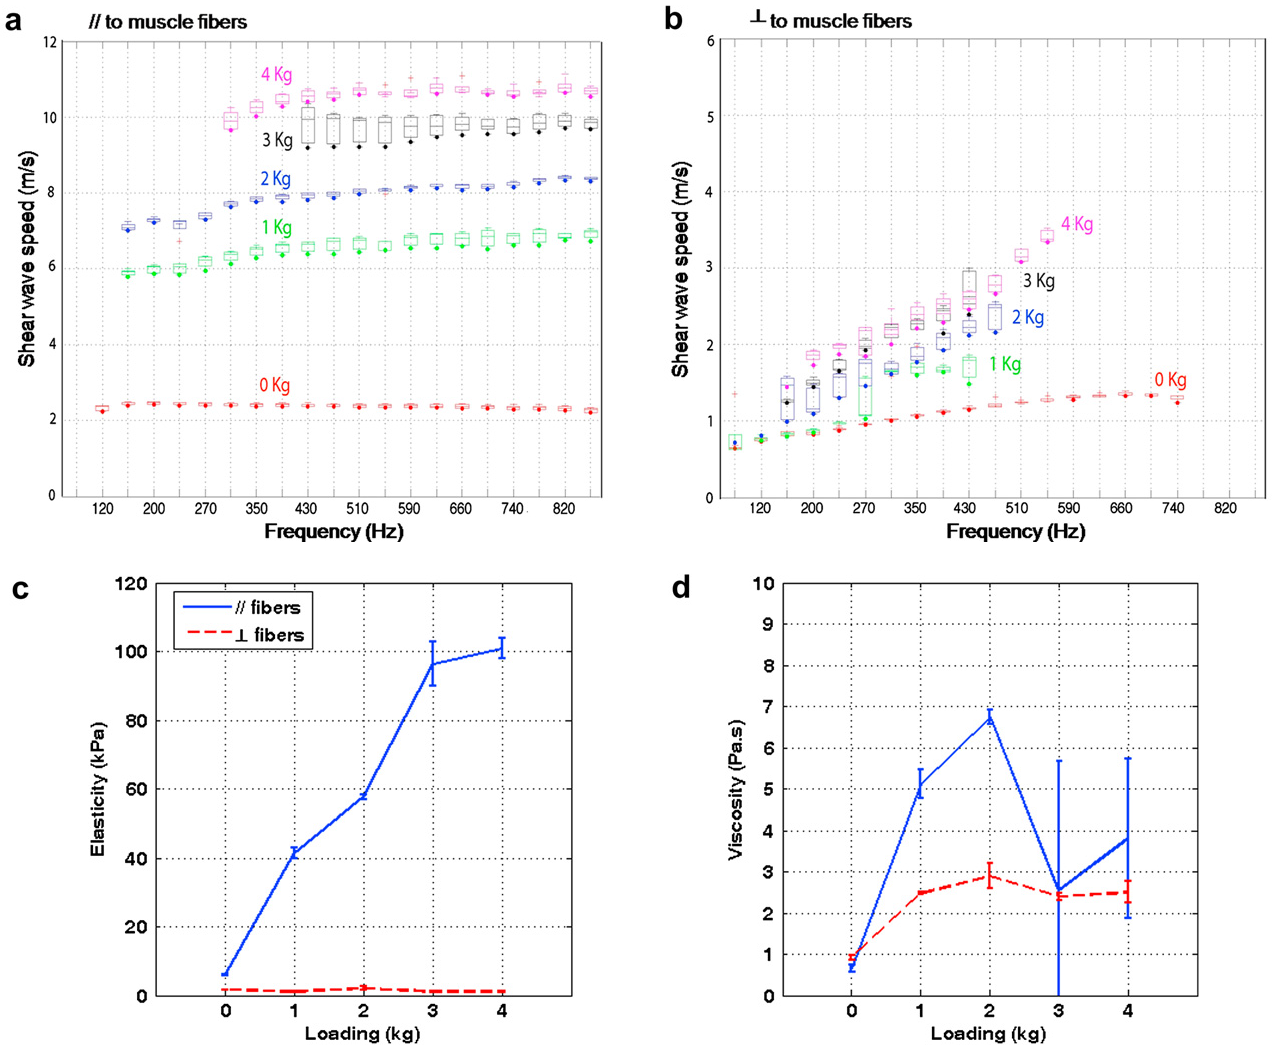
\includegraphics[width=.90\linewidth]{Figures/elastography/gennisson_dispersion2.png}
	\caption{Shear wave speed and estimated mechanical properties for the human \textit{brachialis} muscle under various loads, with elbow flexion of \SI{90}{\deg}. \textbf{(a,b)} Shear phase velocity over frequency under various loads for one subject, \textbf{(a)} parallel to muscle fibres and \textbf{(b)} perpendicular to muscle fibres. \textbf{(c,d)} Estimated mechanical properties using a Voigt model under increasing load, \textbf{(c)} shear elasticity and \textbf{(d)} shear viscosity. Figure adapted from \citet{gennisson_viscoelastic_2010}.}
	\label{fig:rem_gennisson_dispersion_force}
\end{figure}


\citeauthor{gennisson_viscoelastic_2010} used both SSI and SWS to assess the mechanical properties of the \textit{brachialis} muscle under various conditions \cite{gennisson_viscoelastic_2010}. The elastic properties were assessed parallel and perpendicular to the muscle fibres, with the elbow at \SI{90}{\deg} flexion under isometric contraction of the \textit{brachialis}, with loads increasing from 0 to \SI{5}{\kilogram} with increments of \SI{1}{\kilogram}. It was found that shear modulus $\mu$ increased with contraction level from 4.0 to \SI{36.6}{\kilo\pascal} along the fibres and from 2.3 to \SI{4.0}{\kilo\pascal} perpendicular to the fibres, highlighting the anisotropic properties of muscle tissue. SWS was also performed under the same load conditions as SSI. It was found that the shear wave phase velocity only increased slightly with frequency parallel to the muscle fibres (similar to findings \citet{deffieux_shear_2009}), but strongly perpendicular to the fibres (see \autoref{fig:rem_gennisson_dispersion_force}a,b). The muscle can thus be considered non-dispersive parallel to the fibres under these conditions (elbow flexion \SI{90}{\deg}). SSI was also performed to assess the passive properties of the muscle, by increasing the elbow angle from 90 to \SI{165}{\deg} with steps of \SI{25}{\deg}. It was found that the shear wave group velocity increased strongly from \SI{2.7}{\meter\per\second} to \SI{5.7}{\meter\per\second} along the fibres, and slowly from \SI{1.2}{\meter\per\second} to \SI{1.8}{\meter\per\second} perpendicular to the fibres (\autoref{fig:rem_gennisson_dispersion_passive}a). The viscoelastic parameters resulting from the dispersion analysis are depicted in \autoref{fig:rem_gennisson_dispersion_passive}b. %It can be seen that the shear elasticity increases strongly with elbow angle, which is in correspondence 


The SWS method has been used to compare the dispersion in stroke-paretic muscles to contralateral muscles during passive \cite{rasool_altered_2016} and active \cite{saadat_frequency_2018} conditions. In study of \citeauthor{rasool_altered_2016}, the biceps muscle was fixed to an elbow flexion angle of \SI{120}{\deg} in a passive state (validated by EMG activity measurement), and SSI and SWS measurements were conducted. It was found that the group velocity was significantly higher in stroke-affected muscles, indicating increased stiffness. Furthermore, a difference in dispersion was found, the phase velocity was observed to be higher over all frequencies in stroke-affected muscles (not significant) \cite{rasool_altered_2016}. \citeauthor{saadat_frequency_2018} measured the shear wave dispersion under active and passive conditions (0\%, 10\%, 20\% and 30\% of MVC), with elbow flexion of \SI{150}{\deg}. It was found that the shear wave phase velocity was higher across all frequencies in the contralateral muscles with respect to the paretic muscles (see \autoref{fig:saadat_dispersion_paretic}). In the passive condition, the opposite was found, in correspondence with the findings of \citeauthor{rasool_altered_2016} \cite{saadat_frequency_2018}. In neither of these two studies a rheological model was fit to the dispersion curves.


%In 2011, Arda and collaborators (5) performed a study of SWE that included the gastrocnemius and masseter muscles and the supraspinatus and Achilles tendons, in 127 healthy volunteers of both sexes in both the longitudinal and transverse planes, to determine the normal measurement values of different healthy tissues. 



% GENNISSON 2
\begin{figure}[t]
	\centering
	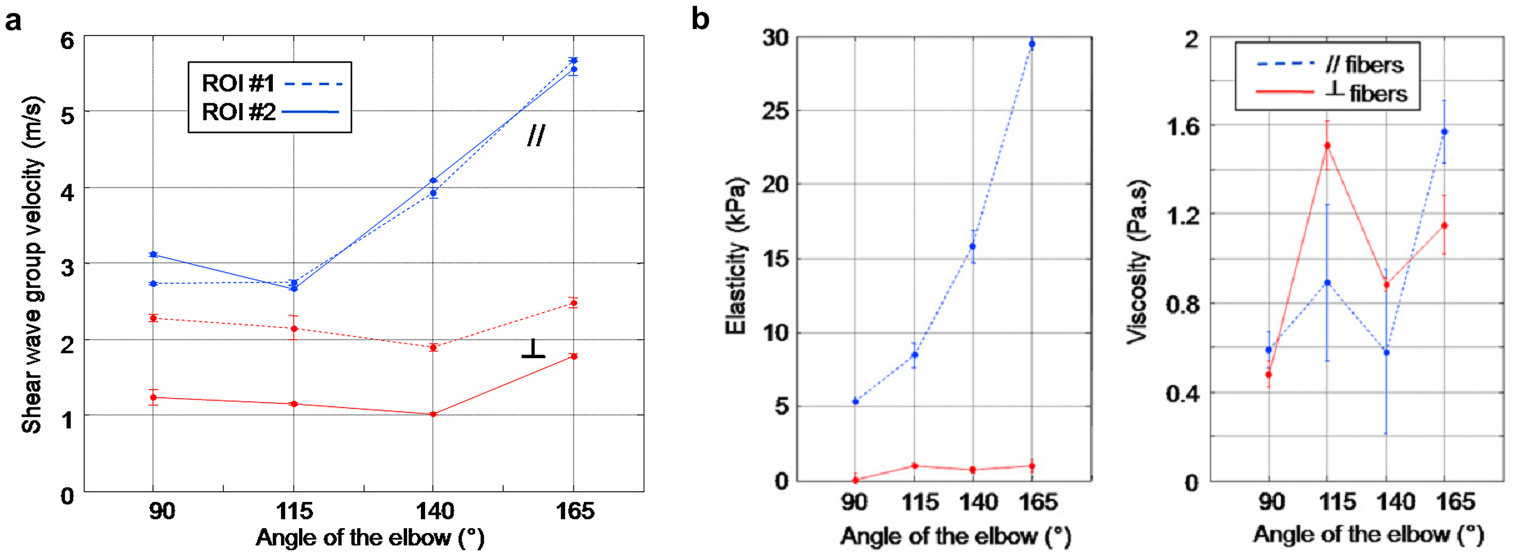
\includegraphics[width=.95\linewidth]{Figures/elastography/gennisson_dispersion_passive.png}
	\caption{\textbf{(a)} Shear group velocity in the  \textit{biceps brachii} (ROI 1) and \textit{brachialis} (ROI 2) along and perpendicular to the muscle fibers, for different levels of elbow extension. \textbf{(b)} Estimated viscoelastic parameters for the \textit{brachialis} muscle. Figure adapted from \citet{gennisson_viscoelastic_2010}.}
	\label{fig:rem_gennisson_dispersion_passive}
\end{figure}

% SAADET
\begin{figure}[t]
	\centering
	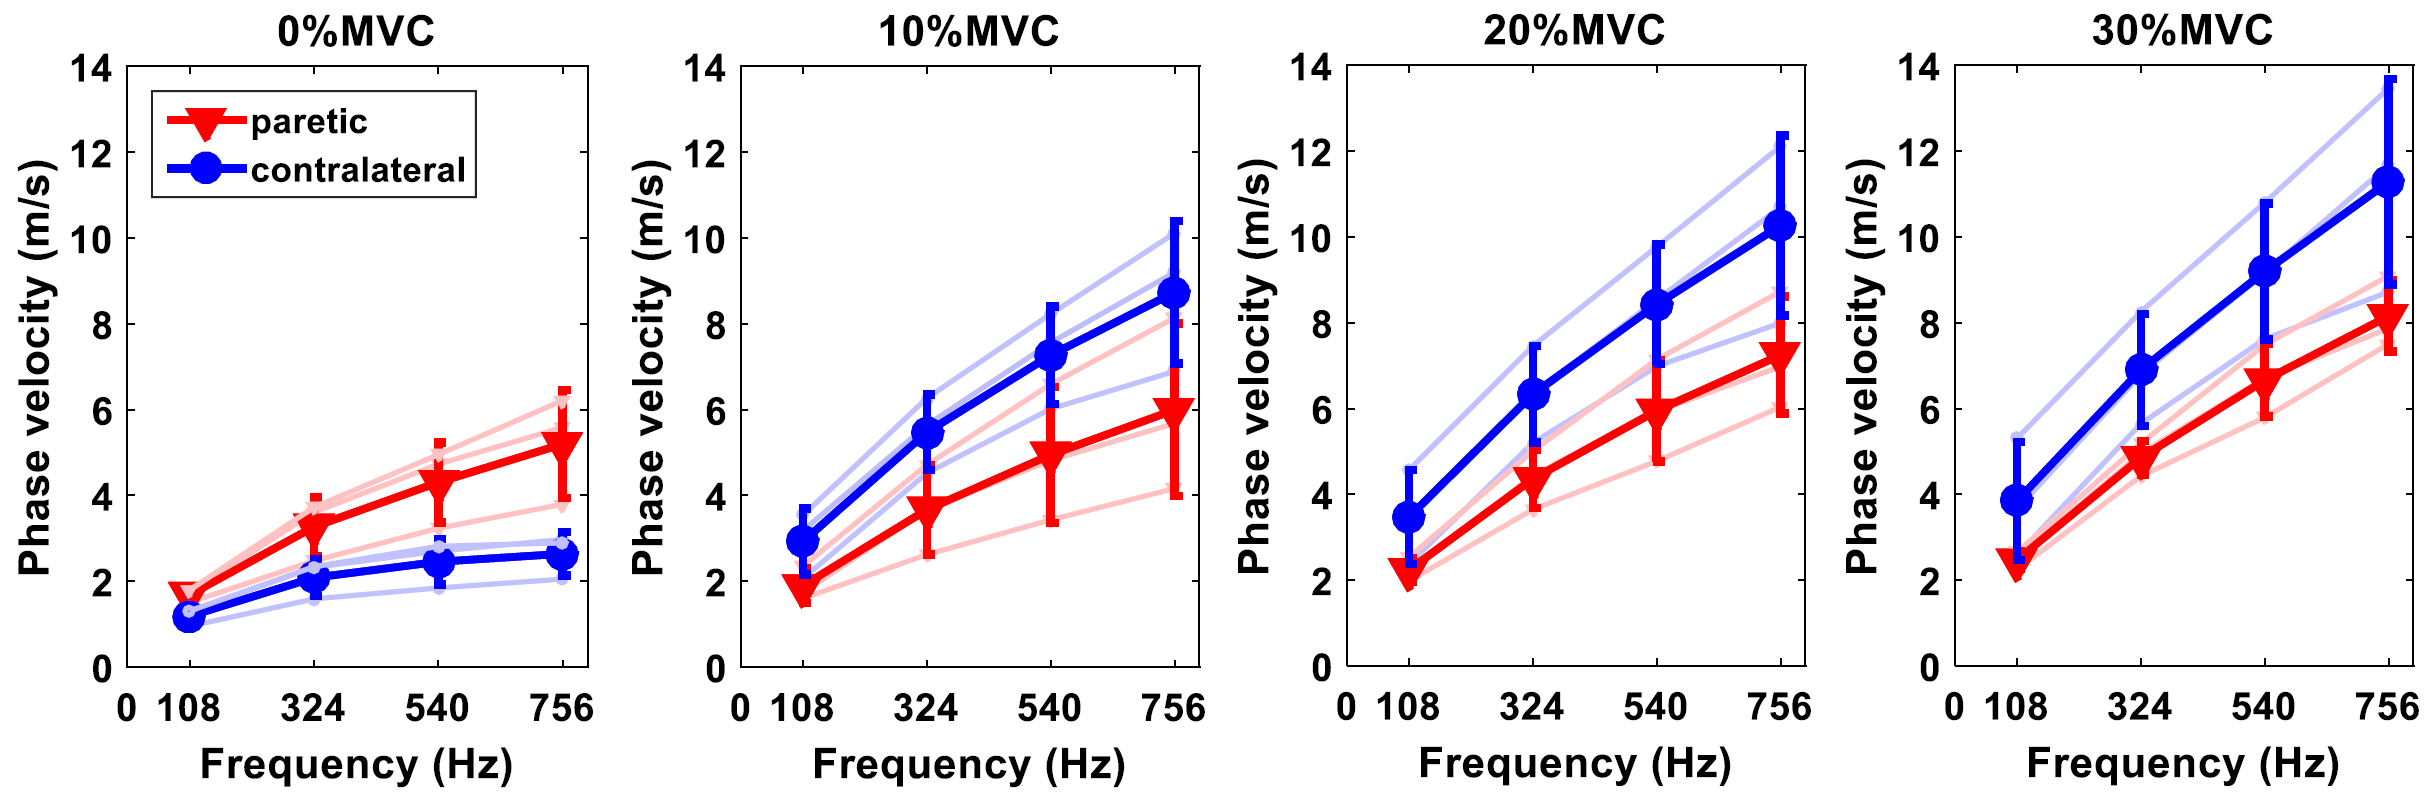
\includegraphics[width=.95\linewidth]{Figures/elastography/saadat_dispersion_paretic.png}
	\caption{Shear wave phase velocity in the biceps muscle over frequency (elbow flexion \SI{150}{\deg}), for multiple levels of contraction. It can be seen that in all the active conditions the phase velocity is lower over all frequencies for paretic muscles compared to the contralateral muscles. Figure adapted from \citet{saadat_frequency_2018}.}
	\label{fig:saadat_dispersion_paretic}
\end{figure}


\subsubsection{Conflicting reports on muscle dispersion}
In the studies by \citeauthor{deffieux_shear_2009} (\textit{biceps brachii}, experimental conditions not described) and \citeauthor{gennisson_viscoelastic_2010} (\textit{brachialis}, elbow \SI{90}{\deg} flexion) the muscle was found to be nondispersive parallel to the fibres (both studies from the group of Tanter and Fink) \cite{deffieux_shear_2009, gennisson_viscoelastic_2010}. By contrast, \citeauthor{rasool_altered_2016} and \citeauthor{saadat_frequency_2018} did found high dispersion when performing SWS parallel to the muscle fibres \cite{rasool_altered_2016, saadat_frequency_2018}. A later study by \citeauthor{rasool_shear_2018}, comparing stroke-affected to contralateral muscles, also reports high dispersion (\textit{biceps brachii}, passive condition, 90, 120 and 150 \si{\deg} elbow flexion) \cite{rasool_shear_2018}. Other than these studies, there are no more studies that performed a dispersion analysis on the SSI measurements from muscles. Furthermore, \citeauthor{rasool_shear_2018} reported a great influence of local minima in optimization procedure (Matlab \texttt{lsqnonlin}, least squares) on estimation of $\mu_1$ and $\mu_2$ parameters of Voigt model to dispersion curves \cite{rasool_shear_2018}. 

%\tred[discussion parameter fit analysis?]



\subsubsection{Estimation of individual muscle force}
\citeauthor{bouillard_estimation_2011} used SSI to estimate individual muscle force in the \textit{abductor digitimi minimi} and \textit{first dorsal interosseous} muscles, and their results were validated by EMG to force conversion methods \cite{bouillard_estimation_2011}. These muscles were chosen because these are muscles without synergists for abduction. Consequently, the measured torque could be related to the measured EMG activation. Subjects were asked to perform ramp contraction from 0\% to 30\% MVC for the \textit{abductor digitimi minimi} and 0\% to 60\% MVC for the \textit{first dorsal interosseous}, in a time of \SI{30}{\second}. In a second trial, subjects had to randomly move their finger, while keeping the MVC between the same level as the ramp contractions. EMG and SSI measurements were done on two separate days (separated by 45 hours). The SSI measurements were performed at \SI{1}{\hertz}, which was the maximum sample frequency of the SSI equipment (Aixplorer version 4.2, Supersonic Imagine, Aix en Provence, France). Two separate simple linear models were fitted to estimate the abduction torque from either shear elastic modulus or EMG. It was found that the model based on SSI measurements was significantly more accurate in predicting torque than the EMG model. 
A later study by \citeauthor{ates_muscle_2015} also found a linear relation between shear elastic modulus (measured with SSI at \SI{1}{\hertz}) and muscle torque, but over the entire range of voluntary contraction of the \textit{abductor digitimi minimi} (i.e. 0\% to 100\% MVC) \cite{ates_muscle_2015}. 


\subsubsection{Validation of mechanical properties}
The mechanical properties assessed with elastography cannot be validated \textit{in vivo}, but \citeauthor{eby_validation_2013} conducted a validation study by performing both SSI and traditional material testing on four porcine \textit{brachialis} whole-muscle tissue specimens \cite{eby_validation_2013}. The muscles were stretched at a rate of $\sim{}1.15$\% $L_0$ per second, up to a maximum strain of 15\% $L_0$, during which SSI measurements were performed. The mean shear modulus was found to be \SI{5.81}{\kilo\pascal} at $L_0$ (corresponding to \SI{90}{\deg} elbow flexion), which is similar to the value found by \citeauthor{gennisson_viscoelastic_2010}. The Youngs's modulus was derived from the stress-strain curve. Next, a generalized linear model regression was done, resulting in a mean fit over all the tissue samples of $\mu = 0.1944 E - 3.6760$, with $\mu$ the shear modulus and $E$ the Young's modulus, both in \si{\kilo\pascal} ($p<0.0001$, $R^2 = 0.9374$). The muscle tissue specimens were assumed purely elastic, hence no dispersion analysis was performed and the viscoelastic properties were not assessed.


%Discussion: application to sysID
%When performing SSI, when transducer is not parallel to fibers, $\mu = \rho V_g^2$ does no longer hold (anisotropy) \cite{eby_validation_2013}.




\subsection{Tendon properties}
Assessing the mechanical properties of tendinous tissue is more complex than other tissue for multiple reasons. (1) Tendon tissue is stiff, resulting in high shear wave speeds (10-20 \si{\meter\per\second} \cite{cortes_continuous_2015, helfenstein-didier_vivo_2016}) which requires imaging with a very high framerate to track the shear wave propagation. (2) The shear wave wavelength ($\lambda {\sim}\SI{25}{\milli\meter}$) for the frequency range used in SSI (300-800 \si{\hertz}) is greater than the mean tendon thickness (Achilles tendon $h{\sim}\SI{4}{\milli\meter}$) \cite{brum_vivo_2014}. This results in guidance of the shear waves along and across the tendon due to successive reflections at the tendon boundaries. As a consequence, the group velocity of the shear wave is not necessarily linked to the actual shear modulus, as assumed in SSI. For this reason, a shear wave dispersion analysis in combination with a shear wave guidance model is required to assess the mechanical properties of tendons. 

\subsubsection{Dispersion analysis with shear wave guidance model}
\citeauthor{brum_vivo_2014} described a novel method to determine the viscoelastic properties of the Achilles tendon based on a transverse isotropic model, whereas in `conventional' SWS, the medium is assumed to behave fully isotropic \cite{brum_vivo_2014}. This transverse isotropic model accounted for the anisotropy in the tendon and guided shear wave propagation. The transverse isotropic properties of the tendon were described by seven parameters, of which many were assumed based on \textit{in vitro} bovine Achilles tendon data \cite{kuo_elastic_2001}. It was found that the elasticity can be determined independently of the viscosity in the parallel direction from the shear wave phase velocity dispersion curve \cite{nguyen_assessment_2011, brum_vivo_2014}. To determine the viscosity, the attenuation dispersion of the shear wave has to be measured. However, unbiased measurement of attenuation is hard due to effects of diffraction, and was not attempted. In the perpendicular direction, both elasticity and viscosity could be determined from the phase velocity dispersion curve. 

This method was used by \citeauthor{helfenstein-didier_vivo_2016} to assess the effect of tendon stretching on shear elasticity, assess the variation of probe location (proximal versus distal) and compare the new method to conventional SSI \cite{helfenstein-didier_vivo_2016}. \autoref{fig:helfenstein_disperson_angle}a shows the dispersion curves for various ankle angles for one subject. It was found that the shear modulus significantly increased with ankle dorsiflexion ($p\leq 0.001$). The estimated shear modulus was found significantly higher with the probe at the proximal location compared to distal, regardless of ankle angle. It was found that SSI compared to the new method underestimates the shear modulus, depicted in \autoref{fig:helfenstein_disperson_angle}b and c. 


\begin{figure}[t]
	\centering
	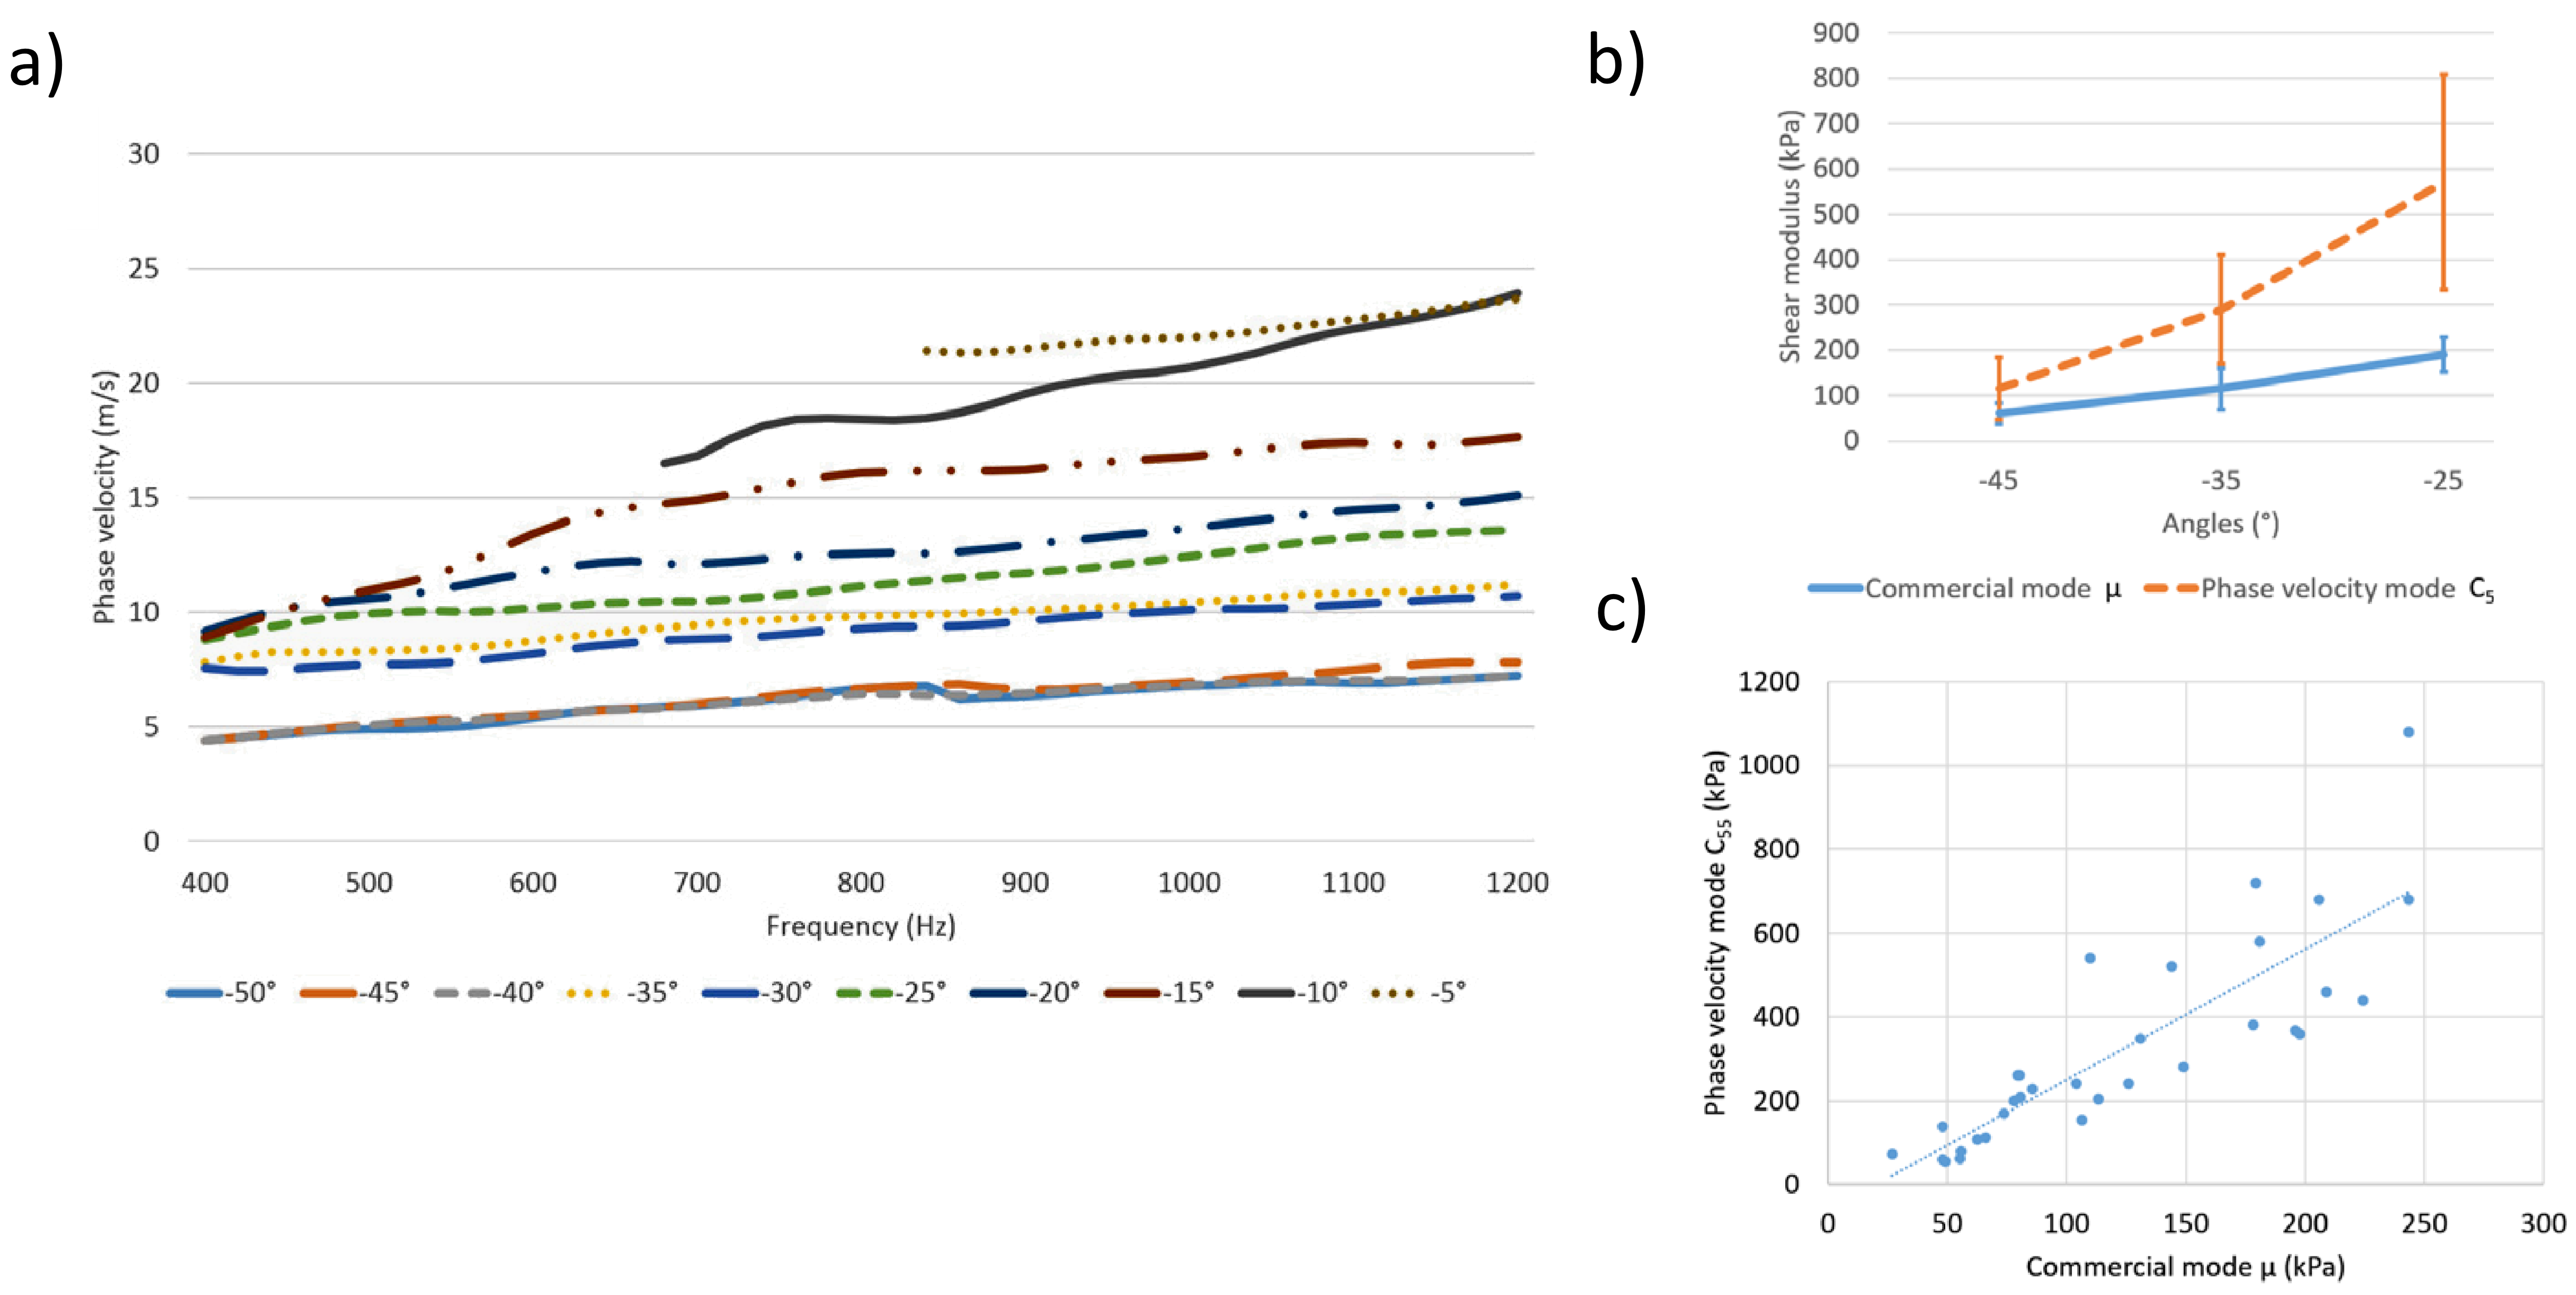
\includegraphics[width=\linewidth]{Figures/elastography/helfenstein_dispersion_angle.png}
	\caption{\textbf{(a)} Shear wave speed versus frequency for various ankle angles, negative angle denotes plantar flexion. Measured phase velocities for frequencies smaller than $c/h$ were removed, where $c$ is the measured shear wave speed and $h$ the mean tendon thickness (which was estimated from B-mode images). \textbf{(b)} Shear modulus assessed with SSI compared to the new method of \cite{brum_vivo_2014} for different plantar flexion ankle angles, \textbf{(c)} the linear relationship found between the two methods (correlation coefficient of $r=0.844$). Figure adapted from \citet{helfenstein-didier_vivo_2016}.}
	\label{fig:helfenstein_disperson_angle}
\end{figure}

\subsubsection{Dispersion analysis without shear wave guidance model}
\citeauthor{cortes_continuous_2015} did also perform a dispersion analysis, however they did not generate shear waves by acoustic radiation force, but used an external actuator in contact with the Achilles tendon via the skin \cite{cortes_continuous_2015}. Furthermore, no shear wave guidance model was used, and thus the viscoelastic properties were determined from the measured dispersion curves (normal SWS method, in conflict with \cite{brum_vivo_2014, helfenstein-didier_vivo_2016}). Using the external actuator, a limited number of frequencies could be excited, from which the dispersion curves could be measured. The induced shear waves were imaged using ultrafast ultrasound. A strong viscoelastic effect was found in the tendon (ankle angle \SI{0}{\deg}), mean values of seven participants were reported to be $\mu_1 = 71.7 \pm 47.2$ \si{\kilo\pascal} and $\mu_2 = 64.6 \pm 13.3$ \si{\pascal\second}. 

	
	%Tendon rate dependency
	%====================================
	%"An important, often overlooked, physiological consideration is the viscous nature of tendons." \cite{seynnes_ultrasound-based_2014}
	%". In humans, a few studies, yet not all (49, 76), have confirmed the rate dependence of tendon mechanics in vivo (42, 74, 91) and in vitro (93); nonetheless, this property remains largely overlooked." \cite{seynnes_ultrasound-based_2014}
	%
	%
	%Nonlinear Force-elongation
	%====================================
	%"Tendon viscoelastic properties, and in particular the nonlinear force-elongation behavior of this tissue, is connected to another methodological challenge: the standardization of stiffness calculation. " \cite{seynnes_ultrasound-based_2014}
	%
	%
	%Tendon (+=muscle) moment arms + force estimation
	%====================================
	%"Unlike in vitro experiments or invasive procedures, the force exerted during in vivo tendon testing can only be estimated."
	%" Like all measurements performed in vivo, the estimation of moment arm length is bound to a number of assumptions that do not invalidate the use of these techniques. " \cite{seynnes_ultrasound-based_2014}
	




\subsection{Shear wave elastography in system identification}
The measurement of the (visco)elastic properties of muscle and/or tendon using elastography might be useful to estimate the force in the MTU, which can then be used to estimate the force in the muscle by using the material model to relate measured displacements to stress. Ultrafast ultrasound has enabled the development of two elastography methods, SSI and SWS. For the former, numerous studies have been conducted to measure the shear wave group velocity in a wide variety of tissues, including muscle and tendon. The latter is used only in a limited number of studies. This section first discusses the reliability of the various studies, followed by a proposed view on how these techniques can be used in system identification experiments. 

	%		- application of these shear wave speeds to system identification is not trivial. 
	%- study that estimates muscle force only demonstrated in very strict experimental conditions, hence questionable if applicable to other muscle groups. should first be demonstrated.
	%- limited frequency of shear modulus estimation, can be increased by using experimental settings. However, fast movement of muscles during identifying reflexes may distort estimation of shear wave velocity, is not demonstrated before. 
The estimation of muscle forces using SSI (\citet{bouillard_estimation_2011}) shows a linear relation between shear modulus and torque, albeit under very specific experimental conditions. During the very slow contraction ramps, SSI measurements at \SI{1}{\hertz} were performed, since this was the maximum sampling frequency of the used equipment. This is too slow for system identification experiments, however, it is known that SSI measurements can be performed at a much higher sampling frequency (by analysing the RF data after the experiment, see \autoref{sec:us_ssi} and \cite{bercoff_supersonic_2004}, sufficient memory assumed). The slow contraction ramps show that it is possible to perform SSI while the muscle is moving slowly, but the contraction velocities encountered during reflexive activity are much higher. SSI measurements in comparable high velocity conditions have not been reported, and are probably impossible to conduct due to distortion of the shear wave on one hand, and the movement of speckles to track the shear wave propagation on the other hand (contribution to movement from both shear wave and contraction, inseparable). Moreover, the method has not been tested for synergistic muscles, so the usability of the method in synergistic muscles remains unknown. 
%estimation of muscle force using SSI \cite{bouillard_estimation_2011,ates_muscle_2015} at 1 Hz only, not usable in sys ID. however, as demonstrated in SSI section, can be performed much faster if beamforming and analysis is not done in real time (which the aixplorer does). Hence, then the estimation of muscle force would be possible at X Hz. However, the muscle is moving a lot faster in sys id experiments than under the conditions of \cite{bouillard_estimation_2011,ates_muscle_2015}, resulting in distorted SSI measurement? Furthermore, this method has not yet been tested in synergistic muscle pairs.


%	- assessment of mechanical parameters can be done before sys id experiment, on muscle or tendon. 
Though the mechanical properties presumably cannot be assessed during the identification experiment, they can be measured prior and after the experiment in tendon and/or muscles. There is however quite some difference in the used elastography methods and reported material parameters across studies, and the results cannot be validated \textit{in vivo}. Given these published results, the applicability of SSI and SWS to quantitatively assess the muscle or tendon properties for system identification purposes remains questionable at the moment. 

	%- two methods (SSI SWS)
%- different reports per method
%- lots of different experimental conditions make results difficult to compare. variety in how results are reported make it difficult to compare. Furthermore differences in subject groups used per study, individual differences subjects make different methdos hard to compare
Especially regarding SWS, there is quite some difference in the used methods to assess the viscoelastic properties of muscle and tendon. There is a lot variety in the experimental conditions used in each of these studies, making it hard to compare them. Furthermore, not every study obtains the same material parameters. For example, where \cite{brum_vivo_2014, helfenstein-didier_vivo_2016} reports that the viscosity of the tendon parallel to the tendon fibres cannot be estimated from the dispersion curves, \cite{cortes_continuous_2015} reports values for both viscosity and elasticity. Moreover, it is hard to assess the influence of individual differences in the tested subjects based on the published literature, when mean values with standard deviation over all the participants are reported. This further hampers the comparison of the studies using SWS.

%- conversion of shear wave velocity to material parameters introduces a lot of assumptions. 
%- SSI relatively easy (Eby), but different 5G = E intead of 3 like in assumed elastic model. 
%- SWS conversion to stiffness not reported before.
%- this makes it perhaps more a qualitative method, based on the rheological model. measured shear wave speed and dispersion are only things that can be seen as qualitative measurements. 
In both SSI and SWS, the tissue is assumed to behave according to a certain rheological model, but validation of these models requires additional research. In case of SSI, a linear elastic isotropic model is used. With this material description, it is possible to estimate the shear elastic modulus from the shear wave group velocity via $\mu=\rho c_g^2$. Following this model, the Young's modulus is equal to $E = 3\, \mu$ (see \autoref{sec:us_ssi}). However, simultaneous material testing and SSI of brachialis swine muscles resulted in a linear fit where $E \approx 5\mu$ \cite{eby_validation_2013}. This shows that SSI can perform well in comparing the shear wave velocity from subject to subject, but results in a more qualitative measurement, than an quantitative assessment of material properties. For SWS, a similar study like \cite{eby_validation_2013} to compare the viscoelastic muscle properties to mechanical tests is not reported. Furthermore, the estimation of muscle force from the shear moduli described by the Voigt model and measured muscle or tendon elongation has not been shown in literature before.
% the conversion of the Voigt model parameters shear elasticity and shear viscosity to mechanical parameters to estimate muscle forces has not been reported.


%		- assessment of muscle properties hard, studies have done it for passive properties of the muscle. Active properties are dependent on activation level, fibre length and velocity, making the estimation of the properties only possible for the force length curve, not force velocity. This limits its usability in sys id experiments.
%		- Alternatively, elastography can be done on tendon, since this is passive material, and thus is not dependent on activation level. However, the tendon is known to behave rate dependent, and has nonlinear force-elongation properties \cite{seynnes_ultrasound-based_2014}. For tendon the same limitation applies as for muscle, that the rate dependence cannot be easily determined. Furthermore, due to the limited thickness of tendons, shear waves reflect at boundaries for low frequencies, distorting the estimation of the viscoelastic properties. 
The reported shear wave velocities for the passive muscle over a range of joint angles show a good correspondence to the expected increase in stiffness \cite{gennisson_viscoelastic_2010}, based on the passive muscle tissue properties \cite{zajac_muscle_1989}. The active properties show a lot more variation (conflicting reports on dispersion), and are more difficult to identify, since they have to be measured for different joint angles and activation levels. Since elastography cannot be performed during eccentric or concentric contraction, the force-velocity characteristic cannot be obtained using elastography. This means that for a muscle, elastography could in theory only be used to separate the active and passive tissue contributions to stiffness in isometric and passive conditions. In dynamic conditions, as presented during system identification experiments, substantial MTU interaction is expected, which further limits the usability of the passive material parameters, because of the many possible combinations of joint angle, activation level and ratio between tendon and muscle length. Although the tendon has only passive properties (i.e. does not depent on activation signal), aforementioned reasons also limit the use of assessed tendon properties, of which the often neglected rate dependency cannot be assessed \cite{seynnes_ultrasound-based_2014}. 



It has been shown that the estimation of shear moduli using SSI varies with transducer pressure and ROI size in both muscle and tendon \cite{kot_elastic_2012}. Furthermore, the shear wave group velocity was found dependent on scanning depth and whether there was bone below the ROI \cite{ewertsen_evaluation_2016}. This calls on one hand for standardisation in performing elastography experiments, by e.g. using casts or mounts for the probe in which the pressure can be properly set and maintained, eliminating interobserver reproducibility issues (reported by e.g. \cite{aubry_biomechanical_2013}). On the other hand this shows the need for further research, e.g. to find the underlying physical principles for the variation dependent on surrounding tissue and depth. 

It can be concluded that before elastography measurements can be of value in system identification, extensive research is needed to find the relation between the estimated shear wave velocity profiles and mechanical properties of muscle and tendon. However, under dynamic conditions, elastography may never be of use, despite technological progress. 


%\subsection{Sources of variation in elastography assessed properties}
%\citet{kot_elastic_2012}
%
%\citet{koo_factors_2015}
%
%\citet{ewertsen_evaluation_2016}
%- using elastography there is variation due to handling of probe, and different technical settings \cite{kot_elastic_2012}
%first e.g. probe mounts have to be developed, and the influence on the quantitative nature of the various  elastograpghy methods has to be further studied, before it is applicable to sys ID. Exact protocols have to be developed...
%
%- abundance of studies uses SSI to assess youngs modulus (e.g. [shinohara 2010, Arda 2011, maisetti 2012], ...see Brandenburg et al. 2014), however the quantitative nature of this measurement cannot be validated in vivo. The in vitro study of \cite{eby_validation_2013} validated this, but did not found the relation $E=3\mu$, but approximately $E=5\mu$. This difference indicates that it might be a more qualitative measurement, but since E is assumed to increase as function of the group velocity squared, the influence on the error in estimation might be limited... 
%
%- for elastography compound imaging can be used to increase image quality, but alternative beamforming methods (Garcia 2013, Montaldo 2009) /RF remapping (check Sumanaweera 2005) can also be used to improve image quality, without decreasing effective frame rate %\cite{cortes_continuous_2015}
%







%\newpage











% ===========================================================================
\section{Separating proprioceptive contribution -- imaging}
Besides elastography, normal ultrafast imaging can be used to track the elongation of muscle fibres, tendon and/or displacement of the myotendinous junction (MTJ). This is expected to be especially useful in understanding contribution of the different proprioceptive afferents to observed movement. 

Ultrafast ultrasound has been used by a number of studies to image skeletal muscle, though the majority of studies use the technology for elastography. Currently, ultrafast imaging has not been used to study reflexes, or to acquire additional data for system identification of the neuromuscular system. Muscle fibre behaviour and MTU interactions during voluntary or electrically stimulated contrations have been studied using ultrafast ultrasound. The findings of these studies will first be presented. 
%In this section first an overview of the findings with ultrafast imaging of the MTU wil be presented. 
Hereafter, studies that used conventional ultrasound to identify the contribution of the components of the MTU (and thus the afferent activity) to reflexes and their findings will be shown. \tred[It will then be discussed in what way ultrafast imaging can help in understanding the origin of the afferent feedback, and in what way it can help to fill the existing gap in knowledge and validation of current hypotheses.] -- \tred[XXX not really relating to system identification, more to identifying stretch reflex]
%% LOCATIONS TO IMAGE
%Imaging can be done at three locations; \textbf{(1)} Over the muscle belly to obtain fibre length of one or more muscles with similar function (e.g. \cite{klint_afferent_2009, cronin_triceps_2015}) 
%\textbf{(2)} Muscle tendon junction, fibre and tendon length (e.g. \cite{klint_afferent_2009})
%\textbf{(3)} Tendon to obtain tendon elongation 


% ===========================================================================
\subsection{Ultrafast imaging of muscle and tendon}
\label{sec:ufus_muscle_tendon}
%Several studies demonstrated the use of ultrafast ultrasound imaging of muscle and tendon during movement, though the identification of reflexes mediated by afferent feedback using ultrafast ultrasound has not been demonstrated before. 

% DEFFIEUX VELOCITY PROFILE
\citeauthor{deffieux_ultrafast_2006} were the first to use ultrafast ultrasound to image the contraction of muscle fibres in vivo upon electrical stimulation (\SI{30}{\volt} for \SI{400}{\micro\second}) \cite{deffieux_ultrafast_2006}. The \textit{biceps brachii} was imaged at \SI{1500}{\hertz}, and using the cross correlation between two successive RF signal recordings the local particle velocity could be assessed, in axial direction (i.e. ultrasound beam transmit direction). This resulted in a particle velocity profile that corresponds to the lateral widening of muscle fibres, instead of their actual shortening. The spatial resolution in the axial direction is much higher than in the longitudinal direction (elaborated further in \autoref{sec:ufus_disc_sys_id}). With this method a maximum particle velocity (i.e. muscle fibre widening) of about \SI{0.7}{\centi\meter\per\second} was found. The muscle fascicle length per frame was not assessed, and due to the fusiform shape and limited size of the ultrasound probe, it is not possible to determine the absolute length of the fibres \cite{hodges_measurement_2003}. Consequently, only relative length changes can be assessed for the \textit{biceps brachii}. This group later performed a study similar to \cite{deffieux_ultrafast_2006}, and named the used tracking technique `echo mechanomyography' \cite{deffieux_assessment_2008}. However, after this last study, the technique has not been reported again. 


% HAURAIX MTU CONTRIBUTIONS DURING ISOKINETIC PLANTAR FLEXION
\citeauthor{hauraix_shortening_2013} used ultrafast ultrasound to determine the contributions of the different components of the muscle-tendon unit during isokinetic plantar flexions \cite{hauraix_shortening_2013}. Imaging was performed at four locations (during four separate trials), over the muscle belly of the medial gastrocnemius and the lateral gastrocnemius, and the myotendinous junction of both these muscles. Six different isokinetic angular velocities (30, 90, 150, 210, 270, and \SI{330}{\deg\per\second}) were used to determine the contributions of MTU components, while ankle angle, velocity and torque were measured. Ultrasound imaging was performed at a maximum of \SI{1000}{\hertz}. One location per trial was imaged, hence each condition was repeated four times to be able to image all the locations. A good repeatability was found for all the conditions, except for the initial \SI{10}{\deg} of motion, which was therefore omitted from the analysis. This allowed all the measurements to be combined, as depicted in \autoref{fig:hauraix_2013}. It was found that the contributions of tendon and muscle to plantar flexion are highly velocity and angle dependent, see \autoref{fig:hauraix_2013_contrib}. 


	% HAURAIX 2013
	\begin{figure}[!t]
		\centering
		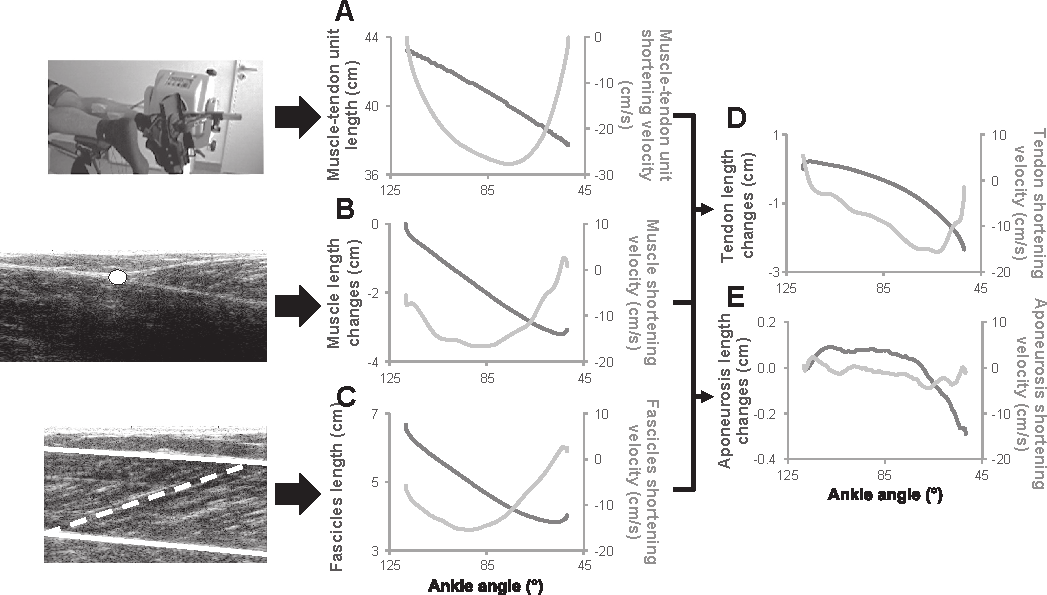
\includegraphics[width=\linewidth]{Figures/mtu_imaging/hauraix_2013_mtu_velocity.pdf}
		\caption{Overview of measured data by \citeauthor{hauraix_shortening_2013} for an isokinetic velocity of \SI{330}{\deg\per\second}. Since the data over the different trials for the different imaging locations showed good repeatability, the data could be combined. \textbf{(A)} From the ankle angle the total MTU length was estimated using as kinematic model. \textbf{(B)} From the ultrasound images the location of the myotendinous junction was tracked, from which the muscle length change was estimated. \textbf{(C)} From imaging over the muscle belly, the muscle fibre length was estimated, using the tracking algorithm of \citet{cronin_automatic_2011}. \textbf{(D)} From the difference in MTU length and muscle length, the tendon length change was determined. \textbf{(E)} Similarly, the aponeurosis length change was determined by the difference in muscle length and horizontal fibre length (i.e. horizontal component of line depicted in (C). Figure adapted from \citet{hauraix_shortening_2013}}
		\label{fig:hauraix_2013}
	\end{figure}
	
	% HAURAIX 2013
	\begin{figure}[t]
		\centering
		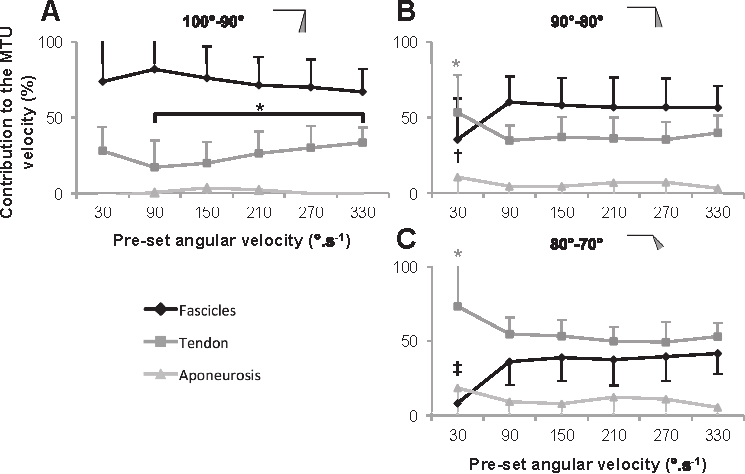
\includegraphics[width=.8\linewidth]{Figures/mtu_imaging/hauraix_2013_mtu_contrib.pdf}
		\caption{The relative contributions of tendon, fibres and aponeurosis for the different isokinetic velocity conditions, at three angle ranges. Significant differences with the fastest isokinetic condition are denoted by * ($P<0.05$), $\dag$ ($P<0.01$) and $\ddag$ ($P<0.001$). Figure adapted from \citet{hauraix_shortening_2013}}
		\label{fig:hauraix_2013_contrib}
	\end{figure}

% FARCY MTU CONTRIBUTIONS QUICK RELEASE GM
Similarly, \citeauthor{farcy_interaction_2014} studied the contributions of the MTU components in quick releasing of the gastrocnemius medialis, from different levels of maximum voluntary contraction (30\% to 80\% MVC) \cite{farcy_interaction_2014}. Ultrafast ultrasound imaging at \SI{2000}{\hertz} was performed with the probe location over the muscle belly, and over the myotendinous junction (again one location per trial). Good repeatability of the measurements (high intraclass correlation coefficients and low coefficients of variation) allowed averaging of the data, and combining the data of the two different imaging locations. It was found that for all MVC conditions, the tendon contributed significantly more ($P<0.01$) to lengthening of the MTU than muscle fibres and the aponeurosis. 
%This holds for all MVC conditions and the complete duration of the quick release trials. 
Furthermore, the relative contribution of the three components did not change with MVC level and the contribution remained constant over the complete trial duration (which was taken as a \SI{25}{\milli\second} window after releasing), except for the first \SI{5}{\milli\second}. 






% ===========================================================================
\subsection{Conventional imaging of muscle and tendon}
There is an abundance of studies using conventional ultrasound to image the muscle or tendon. For example, this has led to the understanding that MTU length is not necessarily representative for muscle fascicle length, and thus for MS Ia and II afferent activity, e.g. \cite{maas_is_2009, cronin_automatic_2011}. In addition, though the frame rate is limited, \tred[many] insights relating to afferent feedback have been reported using this imaging technique. These will be discussed hereafter. 



\subsubsection{Afferent feedback during locomotion}
%expectation? Klint? Sinkjaer? GTO expected more than MS? Timing? Loram? 
%No studies using ultrafast ultrasound for imaging of tendon or muscle displacement. Studies using conventional B-mode ultrasound in abundance.
Ultrasound imaging has been used to assess the muscle fascia length during locomotion by e.g. \citeauthor{klint_afferent_2009} \cite{klint_afferent_2009}. By lowering a hydraulically actuated platform during locomotion, it was found that there was a depression in soleus activity (EMG) at a latency of \SI{42}{\milli\second}, while the muscle fascicle started to differ from the normal walking condition (i.e. no platform drop) after \SI{54}{\milli\second}. This indicates that not MS but GTO feedback via the Ib afferent modulates late stance locomotion. These findings were in correspondence to an earlier study by \citeauthor{grey_positive_2007}, in which plantar flexion perturbations (i.e. rapid unloading) during locomotion were applied directly at the ankle, while tendon force was measured using a buckle transducer \cite{grey_positive_2007}. 



\subsubsection{Stretch reflex}
Tracking of muscle fascicles using conventional ultrasound has also led to new insights in the stretch reflex. \citeauthor{cronin_triceps_2015} found a poor correlation between fascicle stretch (evoked by Achilles tendon tapping and dorsiflexion by ankle dynamometer) of the \textit{triceps surae} and the short latency reflex (SRL) \cite{cronin_triceps_2015}. The poor correlation between the the SLR size and magnitude of both muscle fascicle length and velocity, were in conflict with the earlier belief that the Ia and II afferent muscle spindle activity are the main contributors to characteristic SLR EMG response (e.g. \cite{schuurmans_monosynaptic_2009}). Instead, recorded mechanical vibrations on the skin induced by the tendon taps, were thought to be the main contributor to MS Ia activity. %The tendon taps evoked vibrations in the muscle, which were believed to induce oscillations in the muscle spindles. 
%Same for fascicle velocity, Ia and II afferents thus were found to not really contribute to stretch reflex. Magnitude of applied stretch was not correlated to magnitude observed stretch reflex. 
\tred[MORE oscillation hypothesis...]




%Due to availability ultrasound equipment, and possible interference us waves (?) ultrasound performed at one place. By purely imaging, US can result in tendon length, fibre length, or both. These measurements can be used to estimate the lengthening velocities. 
%However, at one location, only agonist muscles can be imaged, not both at the same time with limited equipment.  



% ===========================================================================
\subsection{Ultrafast imaging in system identification}
\label{sec:ufus_disc_sys_id}
%\textbf{assumptions to Relax}
%\begin{itemize}
%	\item Proportion of contribution of afferent and voluntary can be modelled. Model origin of EMG signal.
%	\item one MTU infinitely stiff tendon
%	\item sources of afferent feedback \tred
%\end{itemize}
%\textbf{intro discussion}

\tred[draft:] To gain a better understanding in how applied mechanical perturbations result in the observed motor behaviour, more data has to be gathered about muscle fibre and tendon behaviour during various experiments. Therefore, first the stretch reflex will be looked at, since it is \tred[thought] to be monosynaptic, and therefore easier to identify then motor behaviour involving many synapses (and voluntary, upper motor neuron... ). 

When looking at the stretch reflex, it is clear that ultrafast ultrasound can be used to determine the latency of muscle fascicle stretch with a higher temporal resolution. In addition to this, ultrafast imaging may also be of use to \textbf{(1)} validate the muscle spindle oscillation hypothesis (which \citeauthor{cronin_triceps_2015} could not test) and \textbf{(2)} measure possible influence of the Ib afferent on the stretch reflex. Methods to validate these hypotheses will be presented. 

The proposed methods could also be used on the ultrasound data that can be acquired in joint dynamic system identification experiments. The use of these methods, and finally, in what way these can help in relaxing assumptions will be discussed at the end of this section.
%Then, these analysis techniques can also be used on the ultrasound data that is acquired in system identification experiments. 


% TABLE AND FIG with spatial resolutions. 
% Table generated by Excel2LaTeX from sheet 'Sheet1'
\newcolumntype{L}[1]{>{\raggedright\let\newline\\\arraybackslash\hspace{0pt}}m{#1}}
\newcolumntype{C}[1]{>{\centering\let\newline\\\arraybackslash\hspace{0pt}}m{#1}}

% Table generated by Excel2LaTeX from sheet 'Sheet1'
\begin{table}[t]
	\centering
	\caption{Properties of different transducer types, and the axial and longitudinal resolution.}
	\small
	\begin{tabular}{L{2cm}C{2.5cm}C{1.8cm}C{1.8cm}C{1.8cm}C{1.8cm}}
		\toprule
		Transducer      & {center frequency [MHz]} & {number of elements} & {max depth [mm]} & {axial res. [\si{\micro\meter}]} & {longitudinal res. [\si{\micro\meter}]} \\
		\midrule
		L12-5 50mm      & 7.813           & 256             & 77              & 19.7            & 195 \\
		L12-5 38mm      & 7.813           & 192             & 77              & 19.7            & 195 \\
		L38-22v 18mm    & 30              & 256             & 20              & 5.1             & 69 \\
		\bottomrule
	\end{tabular}%
	\label{tab:addlabel}%
\end{table}%

\begin{wrapfigure}{r}{0.35\textwidth}
	\centering
	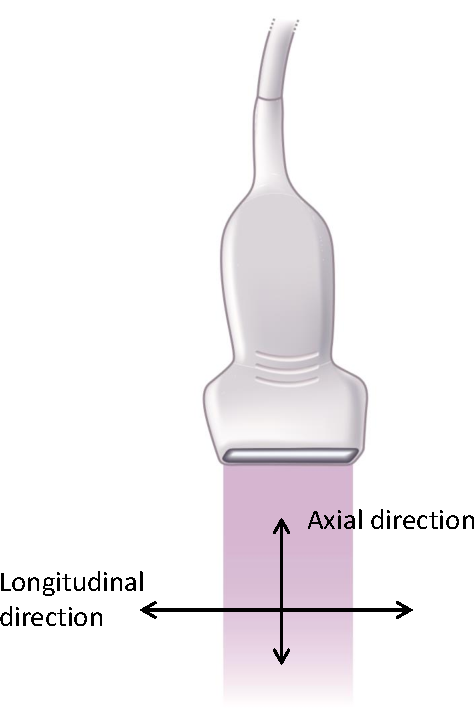
\includegraphics[width=0.9\linewidth]{Figures/Ultrasound/us_res_probe.pdf} 
	\caption{Overview of the important directions in 2D ultrasound imaging. The axial direction is the direction in which the beam is emitted, and the direction perpendicular to this in the imaging plane is referred to as the longitudinal direction. Figure edited from \citet{martin_basic_2011}.}
	\label{fig:usresprobe}
\end{wrapfigure} \leavevmode

%
%\begin{figure}
%	\centering
%	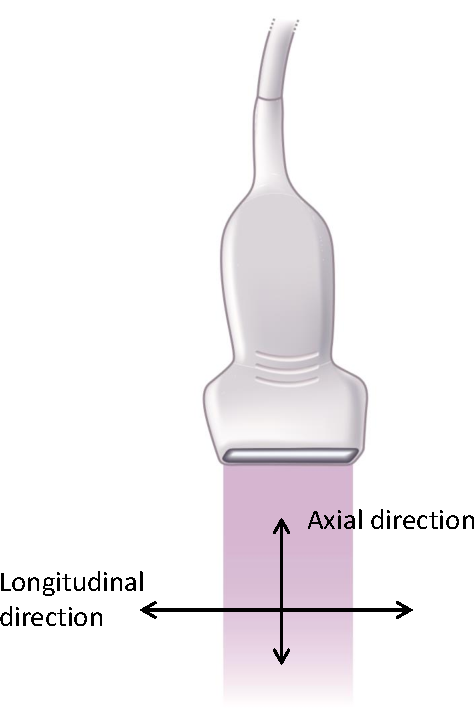
\includegraphics[width=0.3\linewidth]{Figures/Ultrasound/us_res_probe.pdf}
%	\caption{Figure edited from \citet{martin_basic_2011}.}
%	\label{fig:usresprobe}
%\end{figure}



\subsubsection{Spatial resolution ultrafast ultrasound}
The spatial resolution that can be achieved is largely dependent on the type of probe that is used. Furthermore, displacement analysis can be done using two techniques, that are fundamentally different. On one hand, beamformed images can be used, in which the movement of groups of pixels can be tracked. This method is used in most studies that track muscle fascicle behaviour under dynamic conditions, and can be applied to both conventional and ultrafast ultrasound (e.g. \cite{farris_ultratrack_2016, farcy_interaction_2014, hauraix_muscle_2017, af_klint_sudden_2009, cronin_triceps_2015, cronin_automatic_2011}). The spatial resolution in axial and longitudinal direction (see \autoref{fig:usresprobe}) that can be obtained with this method, is indeed dependent on the transducer (number of elements per unit length, frequency) and the number of pixels in the image. 

On the other hand, the raw RF signals recorded from backscattered echoes can be used to detect displacements. This method was called `echo mechanomyography' (see \autoref{sec:ufus_muscle_tendon}) by \citet{deffieux_assessment_2008}. In mechanomyography, \tred[only] displacements in the axial (ultrasound beam) direction can be assessed, by performing 1D cross correlation on the recorded RF signals of successive backscatters. 
%\tred[In comparison with tracking of muscle fibres in beamformed images (e.g. \cite{farris_ultratrack_2016}), the global velocity profiles can be regarded less meaningful. ] \tred[not necessarily less meaningfull, just showing something else. one global, one local...]

% ULTRASOUND SPATIAL RESOLUTION
(about a tenth of the ultrasound wavelength, approx. \SI{150}{\micro\meter} for a probe with a centre frequency of \SI{8}{\mega\hertz}), due to the high sampling rate of the RF data. The spatial resolution in the longitudinal (i.e. probe aperture width) direction is much lower, due to the limited number of piezoelectric transducers per unit length in the ultrasound probe, and the fact that this 



larger in axial then transverse (?) direction (see \autoref{fig:usresprobe}). 

influence probe frequency, width, number of elements per unit length.



\subsubsection{Stretch reflex muscle spindle feedback}
% stretch reflex temporal resolution --> but other approaches possible
%MOVED TO INTRO: {
%When looking at the stretch reflex, it is clear that ultrafast ultrasound can be used to determine the latency of muscle fascicle stretch with a higher temporal resolution. In addition to this, ultrafast imaging may also be of use to \textbf{(1)} validate the muscle spindle oscillation hypothesis (which \citeauthor{cronin_triceps_2015} could not test) and \textbf{(2)} measure possible influence of the Ib afferent on the stretch reflex. }


% muscle spindle osscilation hypothesis: displacement field spectroscopy
%\subsubsection{Muscle spindle oscillation hypothesis}
To validate the hypothesis that muscle spindle oscillations are the main contributor to the observed intensity of the stretch reflex, some of the analysis techniques employed in SSI and SWS may be of use. In SSI, shear waves can be tracked with millimeter resolution in a multiple centimeter wide image \cite{deffieux_shear_2009}. To improve this spatial resolution to be able to perform SWS, multiple experiments are conducted, from which the velocity fields can be averaged. This results in a submillimeter resolution, which allows determining the phase difference of relatively high frequent shear waves ($100-800$\si{\hertz}) over a distance of about \SI{1}{\centi\meter} (see \autoref{sec:us_sws}). 

A similar approach might be applicable to determine the oscillations of muscle spindles, by doing a frequency analysis on the displacement field of the muscle fibres. Evoking the stretch reflex with low variation between trials in one subject (i.e. high repeatability) may be an issue, since a high repeatability in motor response or SLR (M1) latency does not guarantee high repeatability in local fibre deformation (as becomes clear from the fascicle length traces for one subject in Fig. 1 of \cite{cronin_triceps_2015}). On the other hand, this experiment does not need a large probe to induce and follow the shear wave, but a smaller probe with more transducers per unit length can be used \tred[as descibed before.]
 -- XXX \tred[(superficial muscle ???), YES higher frequency probe --> more attenuation, only superficial muscle]. 

Since muscle spindles are $4-7$\si{\milli\meter} in length \cite{smith_chapter_2007}, the ROI to image can be much smaller, allowing to image only a portion of a muscle fibre. It needs to be assessed how representative this local behaviour is for the global muscle movement, and to what extend it is possible to image a single fibre with high spatial resolution. \citeauthor{deffieux_assessment_2008} showed that it is possible to reach micrometer resolution to image muscle contractions \cite{deffieux_assessment_2008}, and given the presumption that muscle spindles are sensitive to length changes larger than about \SI{5}{\micro\meter} \cite{cronin_triceps_2015}

 (muscle spindle length $4-7$\si{\milli\meter} \cite{smith_chapter_2007}), \tred[therefore less wide ultrasound probe, i.e. more transducers per unit length increases lateral resolution REF.] Since muscle spindles are sensitive to length changes from \SI{5}{\micro\meter}. 
In SWS shear wave has to be distinguised from steady tissue, where in this case, all movement that occurs is of interest, but the oscillations have an unknown frequency and amplitude, making it hard to separate them from possible noise (low SNR).
--> problem, out of imaging plane movement, no effect on perturbation frequency?, but has effect on estimation of amplitude oscillation (as in \cite{seynnes_ultrasound-based_2014}, underestimation fibre length). 



\subsubsection{Stretch reflex Golgi tendon organ feedback}
% Ib afferent activity, MTU force hard to estimate
%\subsubsection{}
Stated by Cronin: "Moreover, increasing preactivation torque was often associated with a larger SLR but smaller and/or slower fascicle stretch (Fig. 3)." Preactivation: muscle stiffer, hence elongation more by tendon, raise in MTU force, raise in Ib afferent activity? 
Since it is hard measure or even estimate the force in the MTU, and thus the GTO Ib afferent activity, perhaps an alternative method can be used to estimate the Ib afferent firing. % uitwerken: XXX
Imaging at MTJ, where GTOs are positioned, in transverse plane to find tendon cross sectional area (CSA) over time.  \citeauthor{obst_three-dimensional_2014} found an observable difference in the Achilles tendon CSA between rest and at 70\% (isometric) MVC using conventional ultrasound \cite{obst_three-dimensional_2014}. Perhaps worth exploring if there exists a correlation between tendon thickness and Ib afferent (excitatory) activity. Given the fact that spatial and temporal resolution of ultrafast ultrasound is sufficient to observe the tendon deformation during various contraction conditions. 

% problem with tendon thickness
Tracking the tendon CSA during experiments as the stretch reflex does run into the issue that the tendon is moving, and thus not only the tendon thinning, but also the varying thickness of the tendon will influence the measurement ... VAGUE. This causes an error that cannot be easily discriminated from the thinning (CSA decrease/increase unkown...), tendon CSA over its complete length also unkown, and highly dependent on the state / operating point.

Alternatively, the complete tendon can be imaged, and using speckle tracking the elongation of the tendon can be tracked. Then per location, the tendon thickness can be assessed. Given the fact that the spatial resolution is very high in the direction of the beam when analysing the RF data, this perhaps can be done with sufficient accuracy. I.e. being able to distinguish the elongation/shortening of the tendon and the changes in thickness (in one plane).


\subsubsection{Assumptions introduced by ultrasound imaging}
% Introducing additional assumptions in conformation
It must be noted that while trying to relax some assumptions using ultrafast ultrasound, new assumptions are introduced. The current ultrafast ultrasound equipment can image a 2D plane, in which the muscle fascicle can be tracked. However, in pennate muscles, the fibers in the muscle will rotate upon active contraction, hence move out of the imaging plane \cite{finni_structural_2006}. This out of plane movement, i.e. 3D conformation of the muscle belly, also appears in tendon, and will lead to a systematic underestimation of length changes \cite{seynnes_ultrasound-based_2014}. Consequently, tracking muscle fascicle to estimate the Ia and II afferent activity can also be underestimated, possibly in a non proportional manner (though as of now the gamma activation and thus MS sensitivity remains elusive). Ultrafast ultrasound can be extended to 3D imaging, as demonstrated by \citeauthor{provost_3d_2014} by creating a 3D plane wave, and performing 3D beamforming, but this is computationaly and memory-wise very expensive \cite{provost_3d_2014}. In the future, this would allow imaging the 3D confirmation of the muscle fibers, and thus accurate estimation of muscle fibre conformation and elongation. 
%When considering the complete MTU this may not directly be of influence, but when tracking muscle fascicle to estimate the Ia and II afferent activity, this may be of importance to take into account.
%Ultrasound imaging, tracking fascicle length introduces new assumptions: fibres move out of imaging plane, but assumed fully in plane %\cite{see discussion!}
%		- Finni - Finni (2006): During a contraction, the fibers in a pennate muscle rotate and there is shear strain in the interface between the muscle fibers (Gans, 1982; Huijing, 1999). 
%		-> US imaging only 2D plane, so out of plane fibre rotation is not taken into account. 
%		-  "Disregarding the 3D conformation of tendon introduces a systematic underestimation of tendon length and thus an overestimation of length changes." \cite{seynnes_ultrasound-based_2014}.



\subsubsection{Relaxing assumptions using ultrasound imaging}
Source of Ia and II afferent feedback. 

Ib afferent? 











% ===========================================================================
\section{Implementation ultrasound measurement in current NMC models}
\label{sec:rem_incompatibility}
The currently published neuromuscular models almost all share the assumptions of lumping all muscles (see \autoref{sec:rem_lumping-muscle}). This lumped structure greatly helps in reducing the number of parameters in the model, but induces a large gap between the defined parameters and their physiological meaning. With ultrafast ultrasound, it is possible to acquire data that is closer to the physiology (i.e. proportional), and therefore not directly compatible with the current parametric neuromuscular models. To use the acquired data to fit a model, either a substantial change in the model structure has to be made, or the experimental conditions have to be adapted. The specific model changes or exact experiment design is beyond the scope of this literature survey, however, some thoughts will be shared.

%When adding the UUS technology to the system identification experiments, this asks for a change in the experiment design and/or the model design. elongation of muscle or tendon measurements cannot be plugged in as input to the currently used model structures (agonist and antagonist lumped). Therefore, or the experiment has to be designed differently, or the model has to be adapted.



\subsection{Change in experiment design}
At the present time, ultrafast ultrasound equipment is very costly. For this reason, it will be assumed that there is only one ultrafast ultrasound device available in a lab. With a single ultrafast ultrasound device, only one side of a limb can be imaged, either the flexor or the extensor. Consequently, it is not trivial to identify the complete neuromuscular system. As a simplification, only one group of muscles could be identified, by avoiding activation of the antagonistic muscle group. This would mean that the joint has to be disturbed at a sufficient distance from the neutral position, to ensure that only the agonist can contribute to the rejection of the disturbance. To validate that the antagonist is not active during the experiment, EMG measurements can be used, as demonstrated in e.g. \cite{kearney_identification_1997, mirbagheri_intrinsic_2000}. The antagonistic MTUs do indeed still have a passive contribution to the movement, which still has to be identified. 

Alternatively, experiments similar to those of \citeauthor{de_gooijer-van_de_groep_estimation_2016} can be conducted \cite{de_gooijer-van_de_groep_estimation_2016}. In these experiments, a sudden strain is applied (participant asked to not interfere), and only reflexive activity in combination with passive properties are expected. These kind of transient experiments do not allow for the classical system identification (perturb system over wide band of frequencies), but could provide a lot of insight on the contribution of MS and GTO feedback, and subsequent force generation. The nonlinear model of \cite{de_gooijer-van_de_groep_estimation_2016} could relatively easy be expanded with an afferent feedback model, and could be useful to explain the observed movement based on the with ultrasound measured tendon or muscle elongation. 
%, apply strain, no voluntary activity, and try to fit reflex activity to activation of single muscle group (flexor or extensor group). Transient experiments under condition, no real sys ID, but could provide more insight in the contribution of GTO and MS
%Experimental conditions in which antagonistic muscle is not active (e.g. \cite{kearney_identification_1997, mirbagheri_intrinsic_2000}). Could be validated by EMG measurement. E.g. only positive torque, so that only agonist muscle is activated. Think of experimetal conditions such that the current model can be used to identify the properties of the agonist muscle, and tendon ... to identify the joint dynamics under those conditions. Real identification experiment over wide band of frequencies. No need to change the model structure (e.g. models as \cite{schouten_nmclab_2008, mugge_rigorous_2010}


\begin{figure}[t]
	\centering
	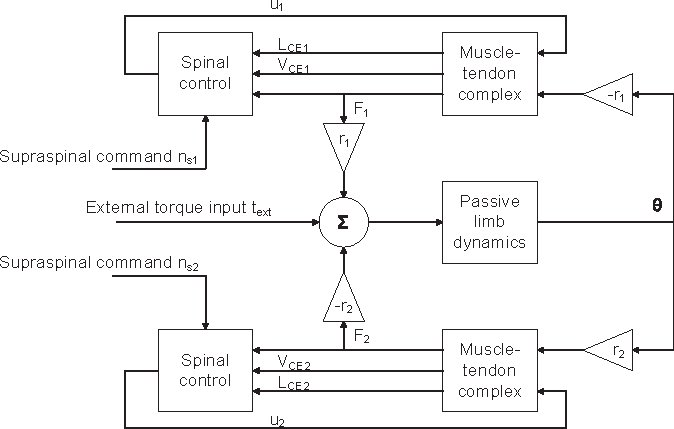
\includegraphics[width=.8\linewidth]{Figures/elastography/mugge_antagonistic.pdf}
	\caption{Antagonistic muscle model used in the simulation study of \citeauthor{mugge_modeling_2012}. The spinal control consists of MS and GTO feedback, and takes an additional supraspinal command as input. The force in the MTU is multiplied by a moment arm to obtain the joint torque. Figure adapted from \citet{mugge_modeling_2012}.}
	\label{fig:mugge_antagonistic}
\end{figure}


\subsection{Change in model structure}
Without a change in experiment design, the model structure has to be made compatible with the additional ultrasound measurement data. One possibility is the introduction of an antagonistic muscle model, like used in \cite{de_gooijer-van_de_groep_estimation_2016}. However, this study did not perform a complete system identification and did not attempt to identify the source of reflexive feedback as mentioned before. Neuromuscular models that include modelling of afferent proprioceptive feedback and antagonistic muscles cannot be found in the context of system identification, but are used in simulation studies, e.g. \cite{munts_fixed_2011, mugge_modeling_2012}. 

The model of \citeauthor{mugge_modeling_2012} (see \autoref{fig:mugge_antagonistic}) is nonlinear and consists of about 50 parameters \cite{mugge_modeling_2012}. It includes the nonlinear properties of the proprioceptors and MTUs (adopted from \cite{winters_analysis_1985, stroeve_neuromuscular_1998}). By contrast, the (linear) model of \citeauthor{schouten_nmclab_2008} consists of 18 parameters \cite{schouten_nmclab_2008}. The difference in linear versus nonlinear modelling makes the comparison unfair, since the linear model is in fact a linearisation of a nonlinear model. However, when considering a linear antagonistic neuromuscular model, this would require (at least) double the number of parameters to describe the MTUs and proprioceptors. In addition, moment arms are required to estimate the net joint torque, introducing at least two additional parameters that are not present in a lumped model. 

In the ideal case, not all of these additional parameters have to be estimated in the parameter fitting procedure. For example, the (average) moment arms could be determined by imaging techniques (MRI, ultrasound \cite{fath_direct_2010}) or estimated based on anthropometric data \cite{ramsay_muscle_2009}. When the relation between shear wave propagation and stiffness or even muscle force is more clearly established, elastography measurements could be used to estimate the tissue (visco)elastic parameters, further relieving the parameter estimation procedure. 

Under the assumption that only one ultrafast ultrasound system is available (costly equipment), only one group of muscles (with the same function) can be imaged during a identification experiment, either the flexors or extensors. Consequently, the sources of afferent feedback can only be estimated for one muscle group. Hence, the antagonistic MTU group remains kind of a black box, in which the MTU interaction cannot be separated. 

The first study that uses ultrafast ultrasound in system identification might have to change the experimental conditions together with the neuromuscular model. 


%In many studies, the muscle tendon unit interaction is omitted, or other methods to estimate the muscle and tendon elongation are used. EXAMPLES, studies that estimate using ankle angle… Not the way to go. The total elongation of the MTU can still be used, and the additional information of US can be used to quantify the individual contribution of lengthening, since one elongation of the (series) system is known. 

%To use this length information, the agonist and antagonist muscles should be modelled separately. But separating these muscle groups faces some difficulties, since the length information of only the agonist MTU is available from the measurement. The antagonistic MTU elongation can still only be estimated as a whole, not individual contributions. 
%Lengthening information of specific muscle can better explain some of the reflexes, but only at for one muscle / muscle group per function. Therefore, the most useful modelling structure will be analysed. 

%A study by \citep{mugge_modeling_2012, munts_fixed_2011} did use an antagonistic muscle model \tred[(INCLUDE MODEL SCHEME)], in which proprioception was included. This was however a (forward) simulation study, and no identification based on measured subject data. These two domains have to be linked, and perhaps UUS can be the bridge. \tred[haha].  

%Mugge et al. used an agonist-antagonistic muscle model to simulate movement patterns (relating to CRPS). This model structure was derived from (Winters \& Stark 1989) and (Stroeve 1998), and consists of an antagonistic muscle pair, both modelled by a Hill model. Describe equations. 

%Using US, there is however the problem that (depending on the equipment available) only one group of muscles (flexor or extensor) can be imaged. So when using two Hill models, the contributions of the other MTU are unknown. This can lead to wrong estimation of MTU elongation, and can lead to problems in identifying the reflexive contributions to movement (further discussed in section afferent feedback)
%Similarly, the intrinsic contributions also become more complicated, since e.g. the intertial contribution has to be split in minimal three components (MTU1, MTU2, limb etc) (further discussed in section intrinsic feedback).





%\subsubsection{Muscle-tedon unit modelling}
%Tendon properties can be assessed with SSI or SWS. 
%relating measurements to muscle force and subsequently joint torque. 
%Several studies not modelled anything, others based on Hill type muscle model. An alternative is the Huxley model, based on crossbridge attachment. 
%
%Hill, Huxley, no model?
%
%Discuss Hill, CE PE SE element. Parameters in model. 
%If antagonistic model is used, one side can be modelled as MTU, in which individual contributions M and T are known. 
%Other side however faces problem, since these separate contributions remain unknown. Here the estimation method employed by Mugge and Schouten perhaps is better. 
%
%
%Alternative, no model 
%Estimate the viscoelastic parameters of tendon (SSI elastography, Supersonic shear wave imaging).
%Measure elongation of tendon. 
%x and xdot of tendon times stiffness viscosity results in force. 
%Tendon properties known to be nonlinear, Finni 2006: “While the tendon force–length curve is non-linear, the Young’s modulus is typically derived from a linear portion of the stress–strain curve (Butler et al., 1978), with an approximate value of 1.2 or 1.5GPa (Zajac, 1989, Alexander, 2002).” 
%Test in multiple ankle positions. ???


 \chapter{Discussion}



- trying to remove assumptions, however important to note that using US and e.g. elastography introduces a lot of other assumptions. So there still is a long way to a completely realistic model. ...
    - Finni - Finni (2006): During a contraction, the fibers in a pennate muscle rotate and there is shear strain in the interface between the muscle fibers (Gans, 1982; Huijing, 1999). 
    -> US imaging only 2D plane, so out of plane fibre rotation is not taken into account. 

-  "Disregarding the 3D conformation of tendon introduces a systematic underestimation of tendon length and thus an overestimation of length changes." \cite{seynnes_ultrasound-based_2014}.



\subsubsection{elastography}
- using elastography there is variation due to handling of probe, and different technical settings \cite{kot_elastic_2012}
	first e.g. probe mounts have to be developed, and the influence on the quantitative nature of the various  elastograpghy methods has to be further studied, before it is applicable to sys ID. Exact protocols have to be developed...

- abundance of studies uses SSI to assess youngs modulus (e.g. [shinohara 2010, Arda 2011, maisetti 12], ...see Brandenburg et al. 2014), however the quantitative nature of this measurement cannot be validated in vivo. The in vitro study of \cite{eby_validation_2013} validated this, but did not found the relation $E=3\mu$, but approximately $E=5\mu$. This difference indicates that it might be a more qualitative measurement, but since E is assumed to increase as function of the group velocity squared, the influence on the error in estimation might be limited... 

- for elastography compound imaging can be used to increase image quality, but alternative beamforming methods (Garcia 2013, Montaldo 2009) /RF remapping (check Sumanaweera 2005) can also be used to improve image quality, without decreasing effective frame rate \cite{cortes_continuous_2015}


\subsubsection{MTU interaction and afferent feedback}
In many studies, the muscle tendon unit interaction is omitted, or other methods to estimate the muscle and tendon elongation are used. EXAMPLES, studies that estimate using ankle angle… Not the way to go. The total elongation of the MTU can still be used, and the additional information of US can be used to quantify the individual contribution of lengthening, since one elongation of the (series) system is known. 



 \chapter{Conclusion}






%% Use letters for the chapter numbers of the appendices.
% \appendix

%\input{appendix-a}


% BIBLIOGRAPHY
\bibliography{Master_Thesis}    % NATBIB
% \printbibliography              % BIBLATEX


\end{document}
%fi